\chapter{\textsc{Moment Unfolding}: direct deconvolution of distribution moments}
\label{chap:moment-unfolding}
\section{Why moments: physics context and QCD calculations}
    Statistical moments of probability distributions serve as powerful tools in physics, providing a concise and theoretically meaningful way to characterise complex phenomena.
    %
    In the context of particle physics, and particularly in quantum chromodynamics (QCD), working at the level of moments rather than distributions offers significant advantages for both theoretical calculations and experimental measurements.
    %
    This section explores the fundamental importance of moments in physics, their theoretical foundations, and their specific applications in QCD.
    \subsection{The Theoretical Significance of Moments in Physics}
        Statistical moments represent a systematic way to characterise probability distributions, with each successive moment providing additional information about the shape and properties of the distribution.
        %
        The $k^{\text{th}}$ moment of a probability density $p(z)$ is defined as
        \[
            \langle Z^k \rangle = \int_{-\infty}^{\infty} z^k\, p(z)\, \dd z
        \]
        While the complete probability distribution contains all available information, working with moments is often much more tractable.
        %
        In many physical theories, moments can be calculated analytically even when full distributions cannot.
        %
        Each moment has a direct physical interpretation---the first moment corresponds to the mean, the second moment to the variance, and higher moments characterize asymmetry (skewness) and peakedness (kurtosis) and so on.
        %
        Moments therefore provide much more concrete insight into the properties of an observable than distributions.
        
        In many physical theories, including QCD, there exist relatively simple evolution equations for how moments change as a function of energy scale.
        %
        If certain moments exhibit universal behaviour across different physical systems, this too reveals universality in the fundamental underlying principles.
        %
        For many physical systems, including those governed by QCD, moments provide a natural language for connecting theoretical predictions with experimental measurements, particularly when examining how observables scale with energy.
    \subsection{Moments in QCD Calculations}
        In quantum chromodynamics, moments play a particularly crucial role in understanding the scaling behaviour of parton distributions and fragmentation functions.
        %
        The DGLAP equations form the theoretical framework for parton distribution function evolution. 
        \subsubsection{DGLAP Evolution Equations}
            The Dokshitzer--Gribov--Lipatov--Altarelli--Parisi (DGLAP) evolution equations~\cite{thomson_modern_2013, Altarelli:1977zs, dokshitzerCalculationStructureFunctions1977, gribovDeepInelasticEp1972} govern how parton distribution functions evolve with energy scale.
            %
            While these equations are integro--differential equations in their most general form, they transform into ordinary differential equations when expressed in terms of moments, significantly simplifying their solution~\cite{Kotlorz:2014fia, Kotlorz:2006dj, Skands:2012ts, dissertori_quantum_2003, Altarelli:1981ax, alma9914845810606531, Gross:1973id, Gross:1973ju, Politzer:1973fx, Moch:2004pa, Vogt:2018ytw}.

            For a parton distribution function $f(x,Q^2)$, where $x$ is the momentum fraction and $Q^2$ is the energy scale, the $n-$th moment is defined as
            \[
                M_n(Q^2) = \int_0^1 x^{n-1}\;f(x,Q^2) \dd x.
            \]
            The DGLAP equations for these moments take the form
            \[
            \frac{\dd M_n(Q^2)}{\dd \ln Q^2} = \frac{\alpha_s(Q^2)}{2\pi}\; P_n\;M_n(Q^2).
            \]
            where $P_n$ are the moments of the splitting functions~\cite{Ellis:1996mzs, salam_elements_2011, Schoeffel:1998tz, Strozik-Kotlorz:2014xga, Simonelli:2024vyh}.
            %
            This formulation converts the complex integro--differential evolution equations into a set of simple ordinary differential equations, one for each moment independently.

        \subsubsection{Operator Product Expansion}
            The Operator Product Expansion (OPE) in QCD naturally expresses deep inelastic scattering structure functions in terms of moments~\cite{Gockeler:2006nq}.
            %
            In this formalism, the moments of structure functions are related to matrix elements of local operators, which have clear physical interpretations and scaling properties.
            %
            For example, the moments of the structure function $F_2(x,Q^2)$ can be expressed as
            \[
                M_n(Q^2) = \int_0^1 x^{n-2}\;F_2(x,Q^2)\;\dd x = \sum_i C_n^i(Q^2) \;\langle O_n^i \rangle.
            \]
            where $C_n^i$ are Wilson coefficients calculable in perturbation theory, and $\langle O_n^i \rangle$ are matrix elements of local operators~\cite{Bardeen:1978yd}.
        \subsubsection{Event Shape Moments}
            Event shape observables, which characterise the geometrical properties of energy flow in collisions, are often studied through their moments.
            %
            Moments of event shapes like thrust, broadening, and jet mass distributions provide sensitive tests of perturbative QCD and allow precise extractions of the strong coupling constant $\alpha_s$~\cite{gehrmann_resummation_2017, Catani:1992ua}.
            %
            The moments of these event shapes can be calculated as
            \[
                \langle e^n \rangle = \int_0^{e_{\text{max}}} e^n \;\frac{1}{\sigma}\; \frac{\dd\sigma}{\dd e}\; \dd e,
            \]
            where $e$ is the event shape variable, and $\frac{1}{\sigma} \frac{\dd\sigma}{\dd e}$ is its normalized differential cross section.
            %
            These moments can be predicted in perturbative QCD, typically expressed as power series in $\alpha_s$:
            \[
                \langle e^n \rangle = A_n \left(\frac{\alpha_s}{2\pi}\right) + B_n \left(\frac{\alpha_s}{2\pi}\right)^2 + \mathcal{O}(\alpha_s^3),
            \]
            plus non perturbative corrections that scale as inverse powers of the centre of mass energy.
    \subsection{Experimental Significance of Moments in QCD}
        From an experimental perspective, moments offer several advantages that make them particularly valuable for QCD studies.

        Some of the most precise determinations of the strong coupling constant $\alpha_s$ come from measurements of moments.
        %
        For example, moments of event shapes measured at LEP have provided determinations of $\alpha_s$ with uncertainties at the few-percent level~\cite{Abbiendi2004Measurementalpha_s, Dasgupta2004EventScattering}.
        %
        Studies by TRISTAN~\cite{Ohnishi1993MeasurementsTRISTAN, Kato1989Double-cascadeAnnihilation}, TASSO~\cite{Althoff1984DeterminationHadrons, Hoyer1979QuantumE+e-, Adeva1983Model-independents}, OPAL~\cite{2005Measurementensuremathalpha_mathrms,Alexander1996QCDGeV, Ackerstaff1997QCDGeV}, DELPHI~\cite{TheDELPHICollaboration2004TheEnergies, SkachkovJinr1994OnCollaborations}, L3~\cite{Achard2002Determination192s208GeV, Heister2004StudiesGeV, Adeva1990TheExperiment, Acciarri1997StudyGeV, Acciarri1996StudyGeV, Acciarri1997QCDCollaboration, Bohm2001MeasurementLeptons, Acciarri2000QCDGeV, Achard2002DeterminationGeV, Achard2002Determination192s208GeV}, and ALEPH~\cite{BuskulicTheCollaboration, Buskulic1997StudiesGeV, Decamp1992MeasurementPredictions} collaborations have all used moment--based analyses to extract $\alpha_s$ values that contribute significantly to the world average.

        The scaling behaviour of moments with energy provides a direct and robust window into the running of QCD couplings.
        %
        By measuring how moments of distributions change with energy scale, experiments can observe the logarithmic scaling violations that are a hallmark of asymptotic freedom in QCD~\cite{Gross:1973id, Deur2016TheCoupling, Abe1990DeterminationApproximation, Farhi1977QuantumJets}.

        Many theoretical QCD calculations are more tractable and more precise for moments than for full distributions.
        %
        For certain observables, perturbative calculations may exist to next to next to leading order (NNLO) or beyond for moments, while full distribution calculations may only be available at lower orders~\cite{Catani:1992ua, gehrmannResummationJetRates2017, Ridder2009NNLOAnnihilation, Chandramohan1981ConsequencesAnnihilation, Catani1991ThrustAnnihilation, Catani1991HeavyAnnihilation}.
        
        In practice, measuring moments directly can reduce certain experimental uncertainties, particularly those related to detector resolution and acceptance effects in regions of phase space with sparse statistics.

        Traditionally, there was no straightforward method to directly unfold moments.
        %
        Instead, moments were computed after first measuring and unfolding the full distribution.
        %
        This typically involved binning the data, unfolding the binned distribution, and then computing moments from the unfolded histogram.
        %
        The limitation of this approach though, is the binning itself, not the moments qua moments.
        
        The use of discrete bins introduces a bias in moment calculations.
        %
        For a variable $z$ binned into $n_{\text{bins}}$ with centers $z_{\text{bin},i}$ and counts $N_i$, the binned approximation of the $k-$th moment is
        \[
            \langle z^k \rangle_{\text{bin}} = \frac{1}{N} \sum_{i=1}^{n_{\text{bins}}} N_i z_{\text{bin},i}^k
        \]
        This approximation introduces a bias relative to the true moment, which grows with the order of the moment computed, and is particularly large in regions where the distribution varies rapidly within bins.

        These limitations motivate the development of unbinned approaches that can directly unfold moments without first discretising the data, which is precisely the focus of the \textsc{Moment Unfolding} method described in this chapter.
    \subsection{Applications in Jet Physics}
        In the context of jet physics specifically---a central arena for testing QCD---moments of jet substructure observables provide particularly powerful probes of QCD dynamics~\cite{CrispimRomao2024JetAnalysis, Dasgupta2013TowardsSubstructure}.
        %
        Several notable applications deserve special mention.
        
        The energy scale dependence of jet properties is best studied through their moments.
        %
        The moments of jet substructure observables such as jet mass, width, and multiplicity exhibit characteristic scaling with jet energy that can be predicted by perturbative QCD~\cite{Dasgupta2013TowardsSubstructure}. For example, the first moment of the jet mass scales approximately as
        \[
            \langle m^2 \rangle \propto \alpha_s(p_T) \;p_T^2 \;\ln\frac{R}{R_0}
        \]
        where $p_T$ is the jet transverse momentum, $R$ is the jet radius, and $R_0$ is the reference scale~\cite{ManganoINTRODUCTIONQCD, Kodaira1978HowQCD}.
        %
        Higher moments have different scaling behaviours, providing multiple handles on the underlying QCD dynamics.

        The moments of jet substructure variables are also used in the classification of jets.
        %
        This is because jet moments differ characteristically between quark--initiated and gluon--initiated jets, making them valuable for jet flavour tagging.
        %
        For instance, gluon jets typically have higher multiplicity and broader mass distributions than quark jets, reflected in the moments of these distributions~\cite{Butter2023PerformanceTagging, Ali2011JETSQCD, SalehMoghaddam2022ComparisonConstant}.
    
        Jet substructure moments also provide a window to study non--perturbative effects and hadronization.
        %
        The interplay between perturbative and non-perturbative effects in QCD is particularly evident in moments of jet observables.
        %
        Lower moments often capture the perturbative, large--angle radiation physics, while higher moments become increasingly sensitive to non--perturbative effects like hadronisation~\cite{Dokshitzer1996DispersiveProcesses, Salam2001HadronShapes}.
    
        In the context of Soft-Collinear Effective Theory (SCET), moments of jet substructure observables provide direct constraints on the parameters of the effective theory, offering a bridge between first--principles QCD and phenomenological models of jet formation~\cite{Chien2014JetTheory, Ellis2010JetSCET, Lee2006MomentumTheory}.

        \subsubsection{Moments in physics beyond the Standard Model}
            While moments are crucial for precision QCD studies, their utility extends to searches for BSM physics.
            %
            Certain moments of distributions can exhibit enhanced sensitivity to new physics scales.
            %
            For example, higher moments of mass distributions can be more sensitive to heavy particle contributions than the full distribution average~\cite{Buterus2023SomeDistributions, cowan_statistical_1998}.
    
            Moments can therefore provide a model--independent way to parametrise deviations from Standard Model predictions, similar to the role of effective field theory coefficients.
            %
            By measuring a series of moments, experiments can place constraints on a wide class of possible new physics scenarios without committing to specific models~\cite{Li2022MomentsPhysics, Larkoski2020JetLearning}.
            %
            Hence, changes in the moment structure of distributions can serve as an early indicator of anomalous physics, even before the full nature of the anomaly is understood~\cite{Li2022MomentsPhysics, Metodiev2024AnomalyObservables, Romao2021FindingColliders}.

    \subsection{The case for direct \textsc{Moment Unfolding}}
        Given the theoretical significance of moments in QCD and their experimental advantages, there is a strong motivation for developing methods that can directly unfold moments from detector level data without first unfolding the entire distribution.
        %
        Such methods would eliminate binning biases inherent in traditional approaches, while potentially improving precision and reducing computational cost by focusing directly on the quantities of interest.
        %
        They would enable moment measurements in higher dimensional phase spaces where binned approaches become impractical to provide more direct comparisons with theoretical predictions that are formulated at the level of moments.

        The remainder of this chapter presents the \textsc{Moment Unfolding} method, a novel approach that addresses precisely this need by directly deconvolving moments of distributions using machine learning techniques inspired by the Boltzmann distribution and implemented through a GAN like architecture.
        %
        This method offers a significant over extant methods in moment measurements, enabling more stringent tests of QCD predictions and potentially uncovering subtle effects that might be obscured in traditional analyses.
\section{A GAN like method to unfold moments}
    The direct extraction of distribution moments without first reconstructing the entire distribution presents a unique challenge in unfolding methodology.
    %
    Traditional approaches typically reconstruct the full differential cross--section before computing moments, introducing unnecessary computational complexity.
    %
    The \textsc{Moment Unfolding} technique presented in this chapter takes an entirely different approach by directly targeting the moments themselves.

    The basic idea underlying \textsc{Moment Unfolding} is the connection between statistical moments and the Boltzmann distribution from statistical mechanics~\cite{Boltzmann1978AbleitungLichttheorie, Sharp2015Translation1909}.
    %
    In thermodynamics, the Boltzmann distribution represents the probability distribution that maximizes entropy while satisfying certain constraints on average quantities (internal energy). 
    %
    This principle can be adapted for our unfolding problem, where we seek to find a reweighting of simulated events that accurately reproduces the moments of the true particle level distribution.
    \subsection{Boltzmann inspired reweighting}
        The central mathematical construction of \textsc{Moment Unfolding} is a reweighting function inspired by the Boltzmann factor,
        \[
            \label{eq:moment-generator}
            g(z;\,\vb*\beta) = \frac{1}{P(\vb*{\beta})} \exp\left[-\sum_{a=1}^n \beta_a \; z^a\right]
        \]
        where $z$ is the particle level observable whose moments we wish to unfold, $\beta_a$ are parameters to be determined\footnote{analogous to Lagrange multipliers in used by Boltzmann to derive his eponymous distribution}, $P$ is a normalisation factor similar to the partition function, and $n$ is the number of moments we aim to unfold simultaneously.

        This form is particularly powerful because it directly connects to the maximum entropy principle in statistical mechanics.
        %
        Just as the Boltzmann distribution maximises entropy subject to constraints on average energy, this reweighting function maximises the binary cross entropy loss of the discriminator's classification output between the reweighted distribution and the prior distribution while enforcing constraints on the moments.
        %
        When applied to Generation with probability density $q(z)$, this reweighting function produces a modified distribution
        \[
            \widetilde{q}(z) = g(z) \cdot q_(z)
        \]
        The training objective then is to determine the optimal values of the parameters $\beta_a$ such that the moments of reweighted Generation, $\widetilde{q}(z)$, match those of Truth, \(p(z)\).
    
    \subsection{Adversarial training framework}
        Given the theoretical foundation provided by the Boltzmann form, one now needs a practical method to determine the optimal parameters.
        %
        The task can very naturally be framed as a two level optimisation problem.
        \begin{enumerate}
            \item The parameters $\beta_a$ control the reweighting at the particle level, and
            \item The quality of the reweighting must be assessed at the detector level
        \end{enumerate}
        This task is highly non trivial because the detector response function, which maps particle level to detector level observables, is typically stochastic and known only implicitly through simulation.
    
        To address this, \textsc{Moment Unfolding} employs an adversarial training architecture inspired by Generative Adversarial Networks (GANs), but with significant modifications tailored to the unfolding problem.
        %
        Unlike traditional GANs that generate new samples, \textsc{Moment Unfolding}'s ``generator'' does not generate samples.
        %
        Instead, $g(z)$ generates weights that reweight existing Generation events according to the Boltzmann form.
        %
        The discriminator is a neural network classifier $d(x)$ that attempts to distinguish between Data and reweighted Simulation at detector level.

        The system is then trained adversarially, with the generator attempting to fool the discriminator while the discriminator attempts to correctly classify events.
        %
        This setup is illustrated in \cref{fig:schematic}, showing the flow of information and the adversarial training process.
        \begin{figure}
    \centering
    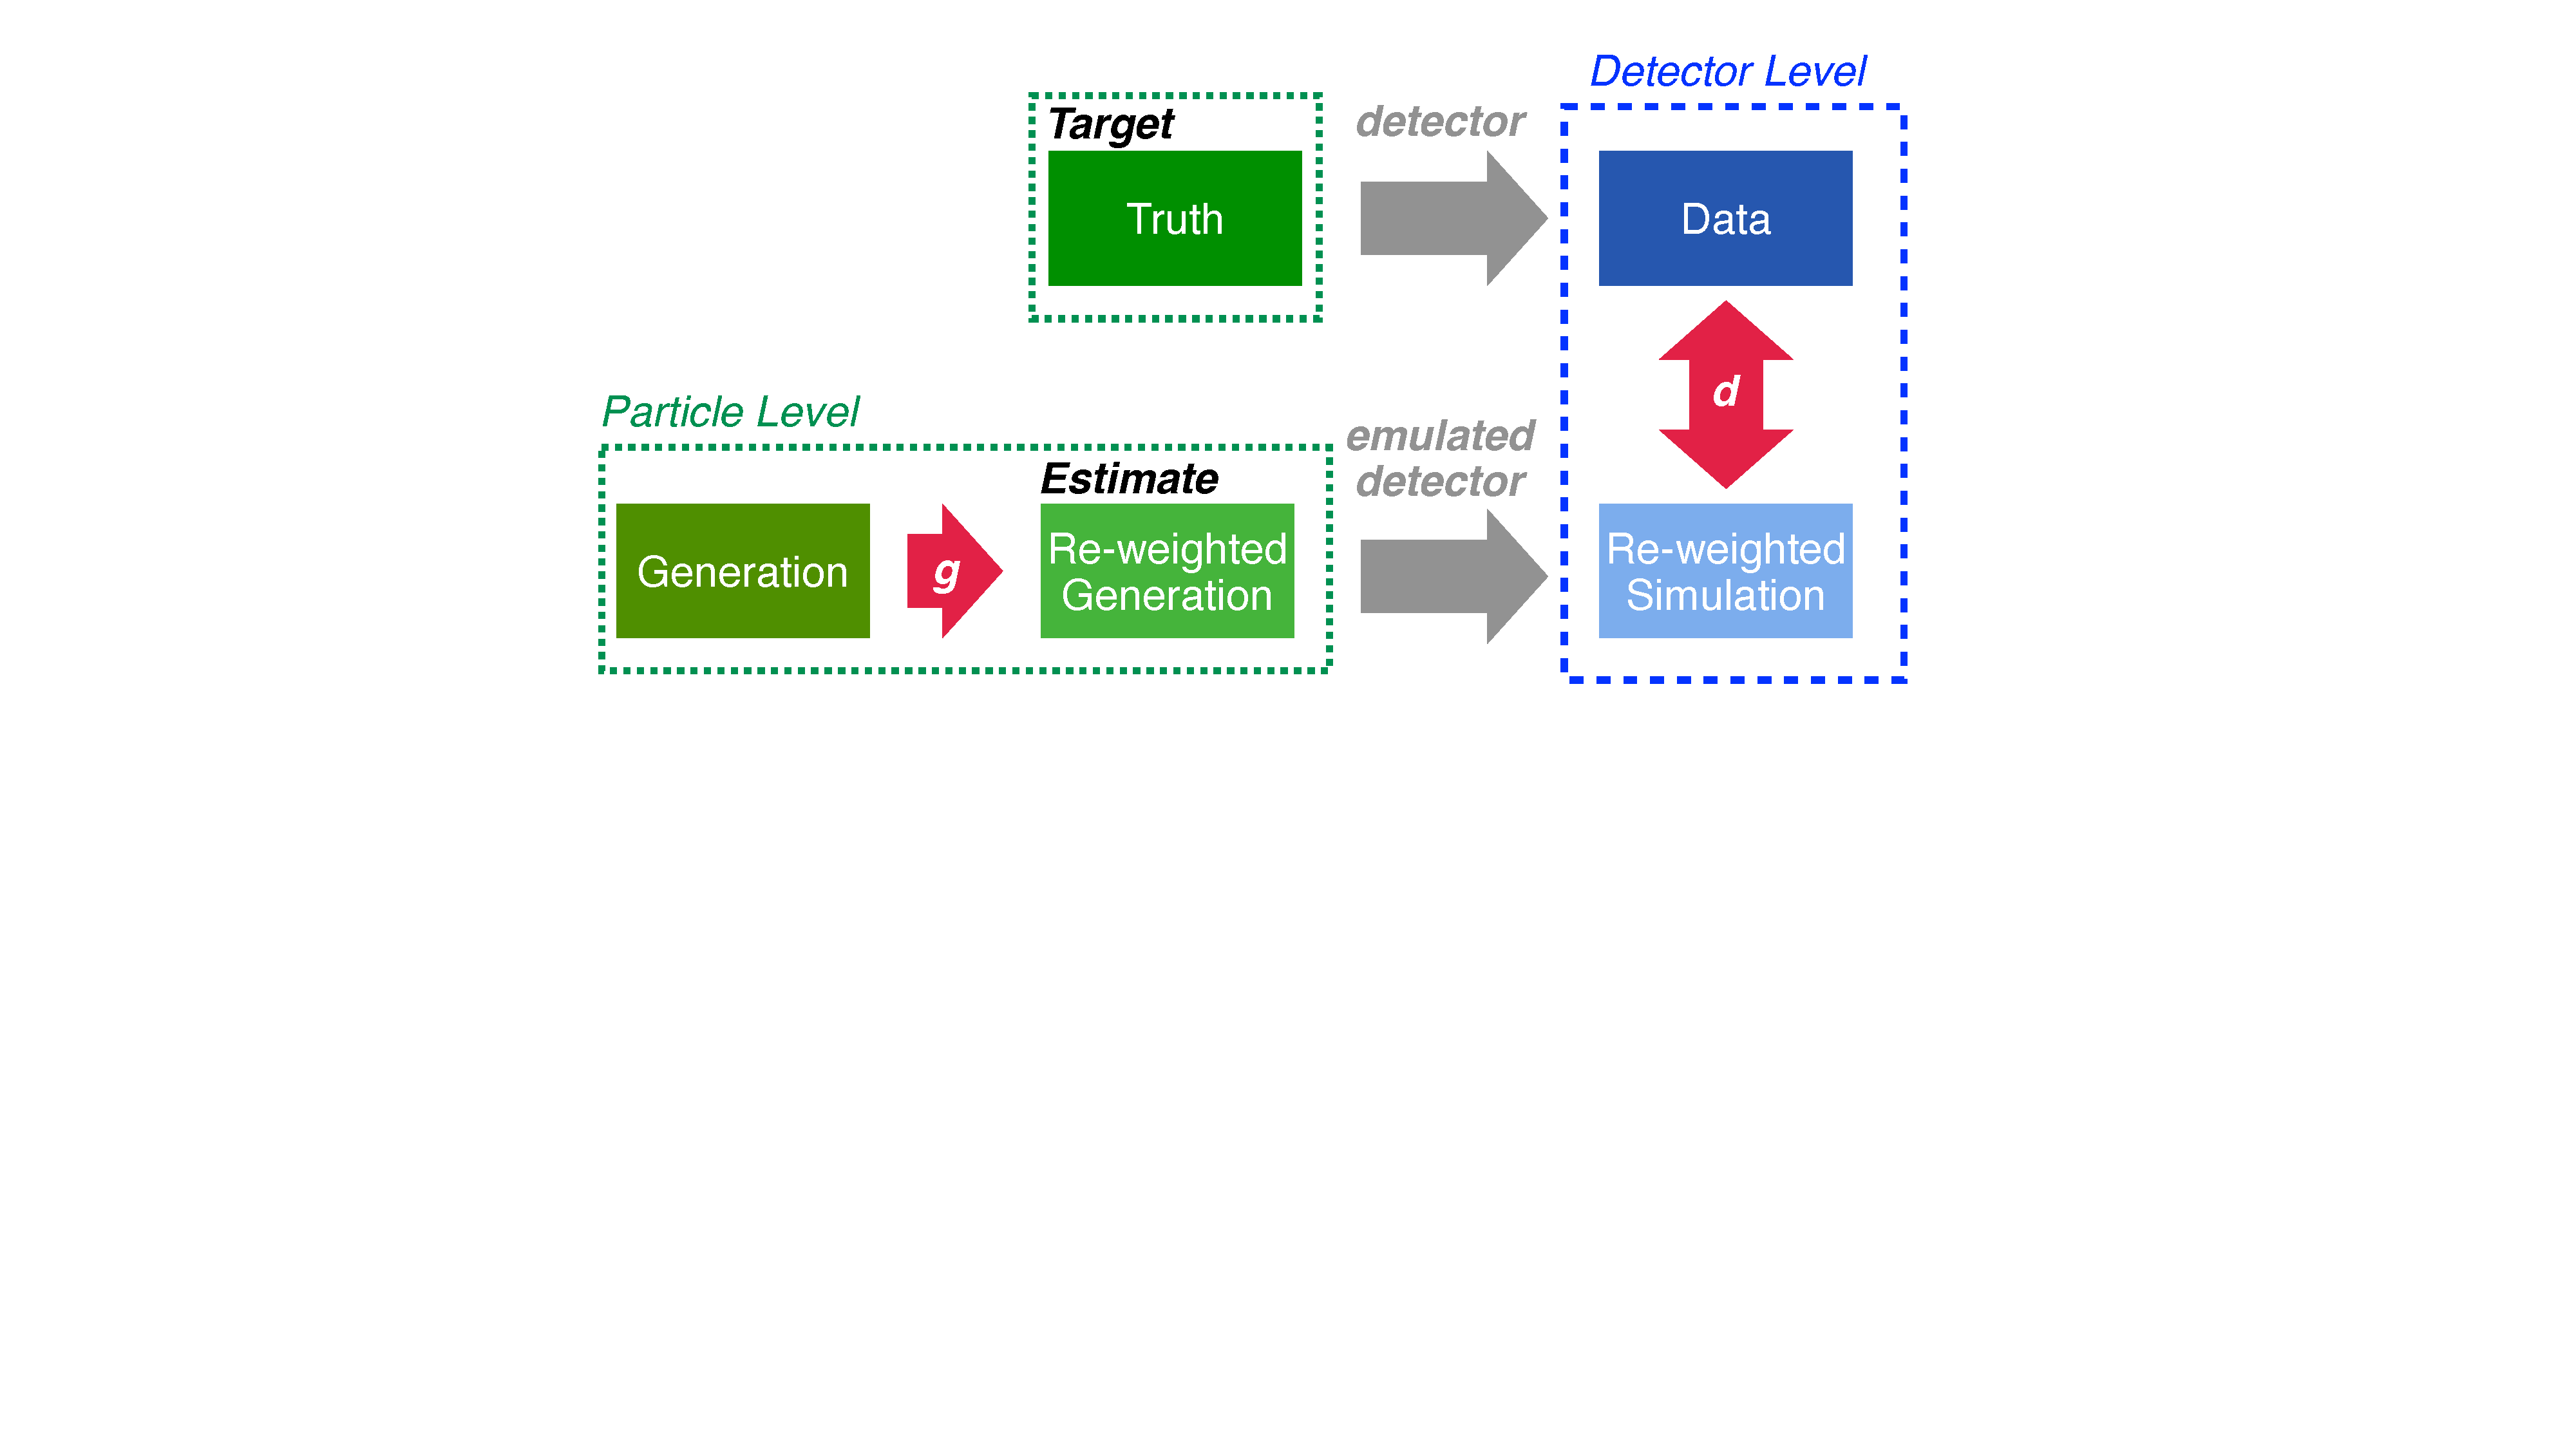
\includegraphics[width=0.90\textwidth]{figures/chapter-05/Schematic_momentunfolding.pdf}
    \caption{A schematic diagram of the training setup for \textsc{Moment Unfolding}.  Like a GAN, $g$ is the generator and $d$ is the discriminator, but unlike a GAN $g$ does not generate samples, it instead generates reweighting factors given by \cref{eq:moment-generator}.  The reweighted Simulation dataset inherits its weight from the matching Generation dataset.  The detector emulations are only run once, since a new simulated dataset is created via importance weights and not by changing the features themselves.}
    \label{fig:schematic}
\end{figure}
        %
        In this framework, the optimal parameters $\beta_a$ are those that make the reweighted Simulation indistinguishable from the Data.
        %
        Once these parameters are found, the moments of the reweighted Generation are the unfolded moments.
    
    \subsection{Mathematical formalism.}
    
        We can formalize the \textsc{Moment Unfolding} approach as follows.
        %
        Let $p(x)$ be the probability density function of the Data distribution and $q(z,x)$ be the joint distribution of particle level and detector level variables in the MC, Generation and Simulation.
        %
        Then $q(z)$ and $q(x)$ are the marginal distributions of Generation and Simulation respectively.
        %
        Let $r(x\,|\,z)$ be the detector response function.
        %
        The assumption of a universal detector response can be formalised as
        \[
            p(x\,|\,z) = q(x\,|\,z) = r(x\,|\,z).
        \]
        The goal is to find parameters $\beta_a$ such that the moments of the reweighted distribution $g(z) \cdot q(z)$ match the true moments of the underlying Truth, \(p(z)\).

        The probaility density function of the reweighted Simulation is
        \[
            \qt(x) = \int g(z)\; \cdot q(z, x) \, \dd z.
        \]
        The adversarial training process optimizes a weighted binary cross entropy loss function,
        \[
            L[g,d] = -\mathbb{E}_{X \sim p(x)}[\log d(X)] - \mathbb{E}_{X \sim\qt(X) }[(1-d(x))]
        \]
        This loss function encourages the discriminator to output high values for real data and low values for reweighted simulation, while the generator is trained to reweight the simulation to make it indistinguishable from real data.

        Once the optimal parameters $\beta_a$ are determined, the unfolded moments can be computed directly from the reweighted Generation
        \[
            \langle Z^k \rangle_{\text{unfolded}} = \frac{\sum_{z \in \text{Gen.}} g(z) \cdot z^k}{\sum_{z \in \text{Gen.}} g(z)}
        \]
        This approach differs fundamentally from traditional unfolding methods that first reconstruct the full distribution and then compute moments.
        %
        By directly targeting the moments themselves, \textsc{Moment Unfolding} is able to avoid both the binning artifacts and dimensionality challenges associated with binned methods and the computational complexity associated with unbinned full distribution unfolding.
    \subsection{Theoretical properties.}
        The \textsc{Moment Unfolding} method possesses several important theoretical properties that justify its application to physics problems.
        %
        Under certain conditions, detailed in \cref{app:mathematical-derivations}, the \textsc{Moment Unfolding} method provably converges to the correct moments.

        The parameter $n$ (the number of moments being unfolded) serves as an implicit regularization parameter.
        %
        By limiting the number of moments, one can constrain the complexity of the reweighting function, helping to stabilise the unfolding process against statistical fluctuations.
        %
        This creates a natural bias--variance trade off: including more moments allows for a more flexible reweighting function but increases sensitivity to statistical fluctuations, including fewer moments leads to stable unfolding but the generator may not have sufficient flexibility to capture interesting features of the data.
        %
        In practice, the optimal choice of $n$ depends on the physics application and available statistics.
        
        \subsubsection{Connection to the maximum entropy principle}
            The Boltzmann form of the reweighting function has a deep connection to the maximum entropy principle in statistical mechanics.
            %
            The reweighting function maximizes the entropy of the reweighted distribution relative to the prior (simulation) distribution, subject to constraints on the moments.
            %
            This provides a principled physical and informational theoretic basis for the method: among all possible reweighting functions that reproduce the target moments, the Boltzmann form is the one that introduces the least additional information beyond what is required by the moment constraints.

    \subsection{Comparison with traditional GAN architectures.}
        While \textsc{Moment Unfolding} draws inspiration from GANs, it differs from traditional GAN architectures, in that the so called ``generator" does not generate data; it generates weights.
        %
        Traditional GANs generate new samples by mapping random noise through a neural network.
        %
        In contrast, \textsc{Moment Unfolding} reweights existing simulated events, preserving the physics correlations already present in the MC and focusing only on correcting the distribution's moments.
    
        Furthermore, unlike conventional GANs where the generator network is incredibly flexible with hundreds of millions of trainable parameters~\cite{brock_large_2019, karras_analyzing_2020, Lee2022BigVGAN:Training}, our generator has an extremely specific parametric form constrained by the Boltzmann expression, with at most a handful of trainable parameters.
        %
        The Boltzmann constraint massively reduces the effective degrees of freedom in the optimisation process and encodes our prior knowledge about the problem structure.
        %
        The parameters $\beta_a$ in the \textsc{Moment Unfolding} approach have clear physical interpretations as Lagrange multipliers enforcing moment constraints.
        %
        This interpretability contrasts with the typically opaque nature of neural network weights in traditional GANs.
    
        Finally, traditional GANs operate at a single level, with the generator and discriminator acting on the same ``type'' of data.
        %
        \textsc{Moment Unfolding} operates across two levels, particle level and detector level, which might not even have the same dimensionality, which is the source of the additional complexity but is essential for the unfolding problem.
        
    \subsection{Practical considerations.}
        While theoretically elegant, the \textsc{Moment Unfolding} method has practical considerations and limitations that must be understood in order to apply the method correctly and effectively.

        Like all reweighting based methods, \textsc{Moment Unfolding} requires that the Generation distribution has overlapping support with the Truth distribution.
        %
        Regions of phase space not covered by the MC cannot be properly unfolded.
        %
        With finite statistics, extremely large weights can arise, in regions of phase space with sparse MC coverage as the generator tries and fails to reweight a zero density into a non--zero density.
        %
        Various regularisation techniques must be employed to mitigate these effects if they arise in a given analysis.
        
        Like other unfolding methods, \textsc{Moment Unfolding} too involves an \textit{ad hoc} choice that must be imposed externally.
        %
        The optimal number of moments to unfold depends on the physics application, available statistics, and the complexity of the true distribution.
        %
        Too few moments may miss important features of the distribution, while too many may lead to overfitting and numerical instabilities.
    \subsection{Extension to differential measurements.}
        An extension of the \textsc{Moment Unfolding} approach is to study moments as a function of another observable, such as transverse momentum.
        %
        This is achieved by making the parameters $\beta_a$ functions of the conditional variable,
        \[
            \label{eq:pt-moment-gen}
            g(z;\,\vb*\beta\qty(p_T)) = \frac{1}{P\qty(\vb*{\beta}\qty(p_T))} \exp\left[-\sum_{a=1}^n \beta_a(p_T)\; z^a\right]
        \]
        This allows the study of how moments evolve with energy scale or other experimental conditions, providing direct comparisons with theoretical predictions of scaling behaviors in QCD.

        The parameters $\beta_a(p_T)$ can be modeled as polynomials, splines, or neural networks, depending on the expected complexity of their dependence on $p_T$.
        %
        This extension significantly enhances the physics applications of the method, enabling studies of how observable moments scale with energy.

    \subsection{Theoretical foundations in statistical mechanics.}
        The mathematical form at the heart of \textsc{Moment Unfolding} has deep connections to statistical mechanics and information theory, providing a solid theoretical foundation for the method.
        %
        In statistical mechanics, the Boltzmann distribution arises as the solution to the maximum entropy problem.
        %
        The maximum entropy problem is the problem of finding the probability distribution that maximizes entropy subject to constraints on expectation values (typically energy).
        %
        The solution takes the form
        \[
            p(s) = \frac{1}{Z} e^{-\beta E(s)}
        \]
        where $E(s)$ is the energy of state $s$, $\beta$ is the inverse temperature, and $Z$ is the partition function.

        The \textsc{Moment Unfolding} algorithm borrows this idea to include multiple constraints on different moments, with each $\beta_a$ serving as a Lagrange multiplier for the constraint on the $a^{\text{th}}$ moment.
        %
        This connection to maximum entropy principles provides a theoretical justification for the specific form of the reweighting function and suggests that it is, in some sense, the most natural choice for the moment unfolding problem.
        %
        The success of this approach in practical applications, as will be demonstrated in subsequent sections, confirms the value of this theoretical grounding and highlights the power of cross--disciplinary approaches in developing new data analysis techniques for particle physics.
\section{Machine learning implementation}
    The theoretical framework introduced in the previous section provides the foundation for \textsc{Moment Unfolding}, but implementing this approach in practice requires careful architectural design and optimization strategies.
    %
    This section details the machine learning implementation that enables robust moment extraction through a GAN like architecture.

    The generator in Moment Unfolding differs fundamentally from traditional GAN generators.
    %
    Instead of producing new samples through a complex neural network, the generator implements the Boltzmann--inspired weighting function, \cref{eq:moment-generator}.
    %
    This function is applied to existing Generation events to reweight them, producing a weighted distribution that matches the moments of the true distribution.
    %
    The parameters $\beta_a$ are the trainable parameters of the generator, and $P$ is a normalisation constant estimated at the batch level,
    \[
        \hat P = \sum_{z \in \text{batch}} \exp\left[-\sum_{a=1}^n\beta_a z^a\right].
    \]

    For differential moment measurements, where the unfolded information is the dependence of moments on another variable like transverse momentum, the $\beta_a$ parameters become functions of $p_T$, as described in \cref{eq:pt-moment-gen}.
    %
    The experiments described below parametrise $\beta_a(p_T)$ as linear functions, 
    \[
        \beta_a(p_T) = \beta_a^{(0)} + \beta_a^{(1)}p_T
    \]
    This linear reparametrisation is motivated by empirical observations that the ratios of spectra between different simulations often exhibit approximately linear dependence on kinematic variables.

    The discriminator network $d(x)$ takes detector level features as input and outputs a probability that a given event came from the real data rather than the reweighted simulation.
    %
    This implementation uses a dense neural network with three fully connected hidden layers with 50 nodes per layer.
    %
    ReLU~\cite{Householder1941ALemmas} activation functions are applied to intermediate layers, and a sigmoid activation function is applied to the output layer.

    This relatively simple architecture provides sufficient capacity to distinguish between data and simulation distributions.

    The training objective is formulated as a weighted version of the Maximum Likelihood Classifier (MLC) loss~\cite{Stoye2018Likelihood-freeEstimator},
    \[
        \label{eq:numericloss}
        L[g,d] = -\sum_{x \in \text{Data}} \log d(x) - \sum_{(z,x) \in (\text{Gen., Sim.})} g(z)(1-d(x))
    \]
    where the first sum is over events from Data and the second sum is over matched pairs of Generation and Simulation events, weighted by the generator function $g(z)$.

    This loss function differs from the standard Binary Cross Entropy (BCE) loss often used in GANs, providing smoother gradients and better convergence properties for our specific application.
    %
    While the BCE loss function could also be used (and indeed gives similar empirical performance), the MLC loss function provides certain theoretical guarantees about the convergence of the method to the correct moments~\cite{desai2024moment}.
    \subsection{Training Procedure}
        The training procedure for \textsc{Moment Unfolding} follows the standard adversarial approach, but with specific adaptations for the reweighting framework.
        
        The generator parameters $\beta_a$ are initialised to small random values near zero, corresponding to minimal reweighting.\footnote{I.e., starting close to the original simulation.}
        %
        The discriminator weights are initialized using standard neural network initialisation techniques\cite{7410480}.
        
        Each training step involves sampling batches of events from Data, Generation, and Simulation.
        %
        The training proceeds by alternating between optimizing the discriminator and the generator.
        %
        First, with the generator parameters fixed, the discriminator weights are updated to minimize the loss function.
        %
        Then with the discriminator weights fixed, the generator parameters are updated to maximize the loss function.
        %
        This alternating optimization continues for a fixed number of epochs, or until convergence criteria are met.

        The \textsc{Adam} optimizer~\cite{kingma_adam_2017} is employed, with an initial learning rate of $5 \times 10^{-4}$ for both the discriminator and generator
        %
        The learning rate is reduced by a factor of 0.5 every 20 epochs to ensure stable convergence.

        To ensure stable training and prevent overfitting, a few regularization techniques are employed.
        %
        Gradient values are clipped to the range $[-1, 1]$ to prevent large updates that could destabilise training, particularly important for the generator parameters which can be sensitive to statistical fluctuations.
        %
        Batch normalisation~\cite{Ioffe2015BatchShift} is applied after each hidden layer in the discriminator to stabilise training and reduce sensitivity to weight initialization and learning rates.
    \subsection{Gradient Updates}
        For the discriminator, gradient computation follows standard backpropagation through the neural network.
        %
        For the generator, gradients are computed with respect to the parameters $\beta_a$ by differentiating the loss function.
        \[ 
            \frac{\partial L}{\partial \beta_a} = -\sum_{(z,x) \in (\text{Gen., Sim.})} \frac{\partial g(z)}{\partial \beta_a}(1-d(x)),
        \]
        where
        \[
            \frac{\partial g(z)}{\partial \beta_a} = -g(z)\left[z^a - \frac{1}{P}\frac{\partial P}{\partial \beta_a}\right] = -g(z)(z^a - \langle z^a \rangle_{g})
        \]
        Here, $\langle z^a \rangle_{g}$ represents the $a-$th moment computed from the reweighted distribution.
        %
        This formulation provides a direct connection between the gradient updates and the moment matching objective of the method.
        
    \subsection{Implementation details.}
        The method is implemented using \textsc{Keras}~\cite{chollet2015keras} with the \textsc{TensorFlow2} backend~\cite{Abadi2016TensorFlow:Learning}, leveraging their automatic differentiation capabilities for efficient gradient computation.
        %
        \textsc{NumPy}~\cite{Harris2020ArrayNumPy} is used for data manipulation, and \textsc{Matplotlib}~\cite{Hunter2007Matplotlib:Environment} is employed for visualisation.

        The computational requirements of \textsc{Moment Unfolding} are remarkably light compared to many deep learning applications.
        %
        Training typically takes less than five minutes per observable on an NVIDIA RTX6000 GPU for the case studies presented in this dissertation.
        %
       Even the potentially computationally intensive calculation of the partition function $P$, which requires summation over all events in a batch is implemented efficiently using vectorized operations in \textsc{TensorFlow}.

        Tab.~\ref{tab:moment-unfolding-hyperparams} summarizes the key hyperparameters used in our implementation.
        %
        These hyperparameter values were determined through systematic experimentation and provide a good balance between training stability and model performance across a range of physics scenarios.

\begin{table}
\centering
\begin{tabular}{|l|c|p{8cm}|}
\hline
\textbf{Hyperparameter} & \textbf{Value} & \textbf{Description} \\
\hline
Discriminator layers     & 3             & Number of hidden layers in the discriminator \\
Discriminator nodes      & 50            & Number of nodes per hidden layer \\
Activation function      & ReLU          & Activation function for hidden layers \\
Output activation        & Sigmoid       & Activation function for the output layer \\
Optimizer                & \textsc{Adam}          & Optimization algorithm used for training \\
Learning rate            & $5 \times 10^{-4}$ & Initial learning rate for the optimizer \\
Batch size              & 10,000        & Number of training events in each batch \\
Training epochs          & 50--100       & Number of full passes through the training dataset \\
Gradient clip value      & 1.0           & Maximum allowed gradient norm for clipping \\
\hline
\end{tabular}
\caption{Summary of training hyperparameters used in the model.
%
These values control the architecture, optimization behaviour, and regularization of the training process.}
\label{tab:moment-unfolding-hyperparams}
\end{table}

    \subsection{Extensions to multiple observables.}
        While the basic formulation of \textsc{Moment Unfolding} applies to moments of a single observable, the method can be extended to handle multiple observables simultaneously.
        %
        For multiple observables $z_1, z_2, ..., z_d$, we can define joint moments as \(\langle z_1^{k_1} z_2^{k_2} \cdots z_d^{k_d} \rangle.\)
        %
        The reweighting function then takes the form,
        \[
            g(z_1, z_2, ..., z_d) = \frac{1}{P}\exp\left[-\sum_{k_1, k_2, ..., k_d} \beta_{k_1, k_2, ..., k_d} z_1^{k_1} z_2^{k_2} \cdots z_d^{k_d}\right]
        \]
        In practice, including all possible joint moments can quickly become intractable as the number of observables increases.
        %
        To address this, one can employ strategies such as
        \begin{itemize}
            \item Limiting the total order of moments (e.g., $k_1 + k_2 + ... + k_d \leq K_{max}$),
            \item Including only specific joint moments known to be physically relevant, and
            \item Using factorised forms that capture the most important correlations while maintaining computational feasibility.
        \end{itemize}
    \subsection{Uncertainty estimation.}
        Accurate uncertainty estimation is crucial for meaningful physics measurements.
        %
        In \textsc{Moment Unfolding}, uncertainties on the extracted moments are obtained through bootstrap resampling.
        %
        Statistical uncertainties are estimated by generating $N$ bootstrap replicas of the data by resampling with replacement,
        %
        applying \textsc{Moment Unfolding} to each replica, and
        %
        computing the standard deviation of the resulting moment values across all replicas.
        %
        This procedure accounts for statistical uncertainties in both the data and the simulation.
        
        Systematic uncertainties related to theoretical modelling, detector effects, and other sources can be evaluated by
        %
        varying the underlying simulation according to systematic uncertainty sources, applying \textsc{Moment Unfolding} to each variation, and
        %
        taking the envelope of the resulting moment values as the systematic uncertainty.

        Such an approach would allow for comprehensive uncertainty quantification that accounts for all relevant sources of uncertainty in the measurement.
    \subsection{Validation procedures.}
        Several validation procedures are employed to ensure the reliability of the \textsc{Moment Unfolding} method.
        %
        Closure tests verify that the method can correctly recover known moments from simulated data.
        %
        The method's internal consistency is verified by checking that the moments computed from the reweighted Generation match the target moments,
        %
        the reweighted Simulation reproduces the features of the Data, and
        %
        that the discriminator is unable to distinguish between Simulation and Data.
        
        Results from \textsc{Moment Unfolding} are also compared with those from traditional unfolding methods like Iterative Bayesian Unfolding followed by moment calculation.
        %
        Agreement between different methods provides additional confidence in the results, while disagreement may indicate methodological issues that require further investigation.
    \subsection{Code availability and reproducibility}
        The implementation of \textsc{Moment Unfolding} is available as open--source Python code, facilitating reproducibility and adoption by the scientific community.
        %
        This open--source approach promotes transparency, enables independent verification of results, and facilitates improvements and extensions to the method by the broader scientific community.
        %
        The full code repository can be found at~\cite{HEP-GAN/MomentUnfolding:Method}, and the specific datasets used for the studies in this dissertation are archived on Zenodo~\cite{AndreassenPythia/HerwigUnfolding}.

    By combining a theoretically motivated approach with practical machine learning implementation details, \textsc{Moment Unfolding} provides a robust and efficient method for extracting moments directly from data.
    %
    The next sections will demonstrate the application of this method to Gaussian data and simulated jet substructure data, showcasing its performance on realistic physics problems.
    
\section{Case studies}
    \subsection{Gaussian experiments}
        Before applying \textsc{Moment Unfolding} to jet physics scenarios, it is essential to validate the method in a controlled environment where the ground truth is precisely known.
        %
        To this end, the approach is first demonstrated using a one dimensional Gaussian example, providing a clear illustration of the method's capabilities while establishing a benchmark for its performance.
        \subsubsection{Experimental Setup}
            For this controlled study, we generate datasets from Gaussian distributions with known parameters.
            %
            The Truth dataset comprises \(\num{10000}\) events drawn from a Gaussian distribution with mean \(\mu_{\textrm{Truth}} = 0.0\) and variance \(\sigma^2_{\textrm{Truth}} = 1.0\).
            %
            The Generation dataset comprises \(\num{100000}\) events drawn from a Gaussian distribution with mean $\mu_{\textrm{Gen.}} = -0.5$ and variance $\sigma^2_{\textrm{Gen.}} = 1.0$.
            %
            Both distributions are then subjected to detector effects modelled as additive Gaussian noise with resolution parameter $\sigma_{\textrm{det}} = 0.5$.
            %
            This setup mimics the typical scenario in particle physics where the MC differs from the true distribution, and both are observed through an imperfect detector.

            \cref{fig:gaussian-setup} illustrates the particle level and detector level distributions, showing how the detector resolution affects both the Truth and Generation datasets.
\begin{figure}
    \centering
    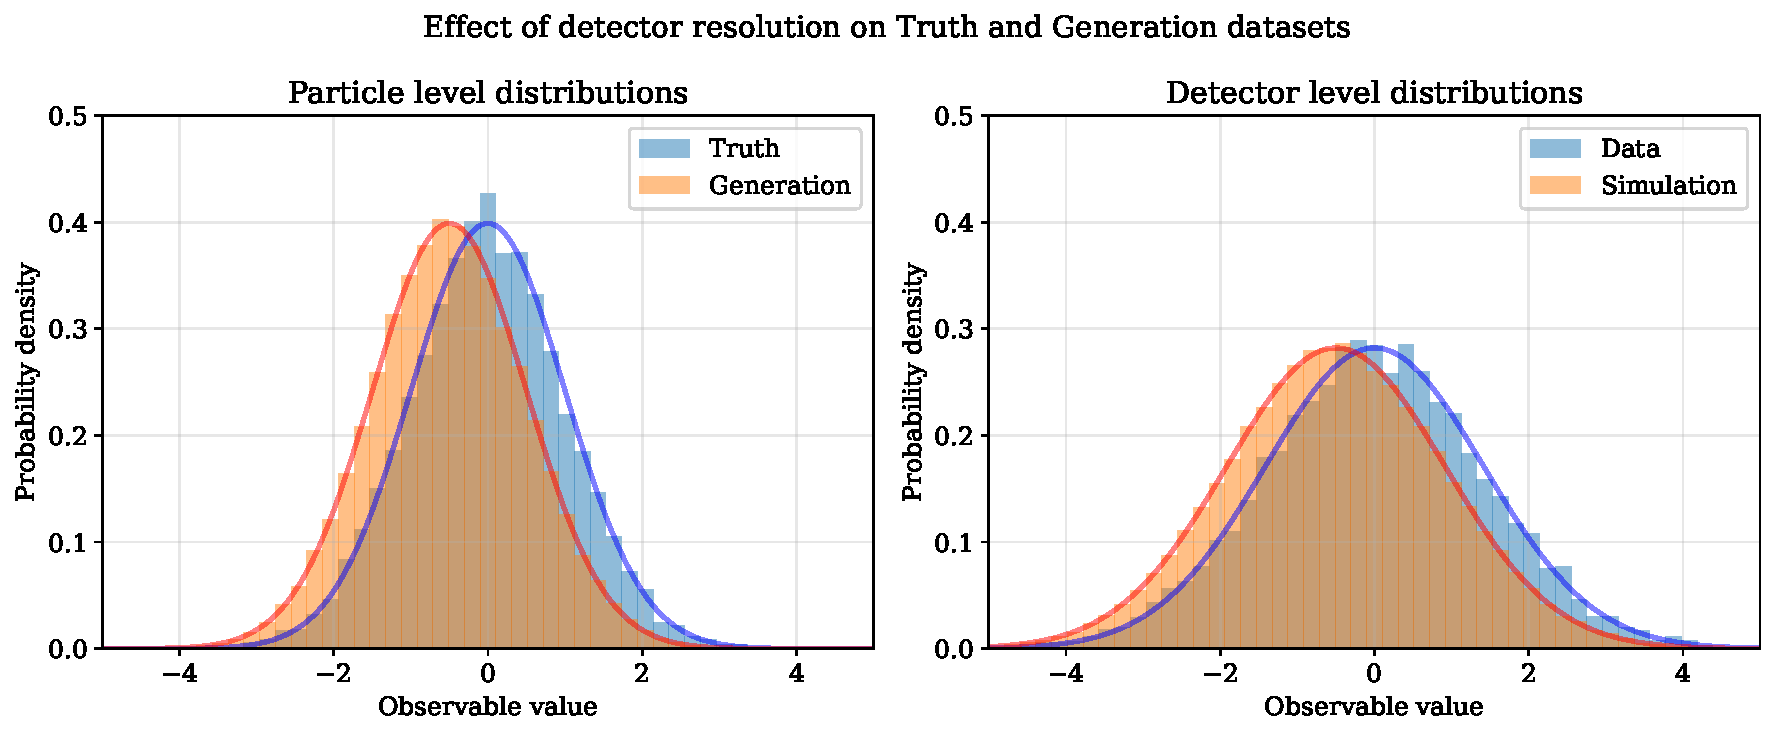
\includegraphics[width=\textwidth]{figures/chapter-05/gaussian-setup.pdf}
    \caption[Effect of detector resolution on Truth and Generation datasets]{%
        Effect of detector resolution on Truth and Generation datasets. 
        The Truth dataset comprises $\num{10000}$ events drawn from a Gaussian distribution 
        with mean $\mu_{\textrm{Truth}} = 0.0$ and variance $\sigma^2_{\textrm{Truth}} = 1.0$. 
        The Generation dataset comprises $\num{100000}$ events drawn from a Gaussian distribution 
        with mean $\mu_{\textrm{Gen.}} = -0.5$ and variance $\sigma^2_{\textrm{Gen.}} = 1.0$. 
        Both distributions are subjected to detector effects modelled as additive Gaussian noise 
        with resolution parameter $\sigma_{\textrm{det}} = 0.5$. 
        \textbf{Left}: Particle level distributions showing the underlying Truth (blue) and 
        Generation (orange) samples before detector effects. 
        \textbf{Right}: Detector level distributions after applying detector resolution, 
        demonstrating the broadening effect while maintaining the relative offset between 
        the distributions. This setup mimics the typical scenario in particle physics where 
        the Monte Carlo simulation differs from the true distribution, and both are observed 
        through an imperfect detector.%
    }
    \label{fig:gaussian-setup}
\end{figure}
        \subsubsection{Results}
            \cref{fig:gauss} shows the results of applying \textsc{Moment Unfolding} to the Gaussian example.
            %
            The left panel displays the particle level distributions, the Truth distribution (blue), the Generation (orange), and the reweighted Generation (black dashed line). 
            %
            Even visually, the close overlap between the Truth histogram and the reweighted Generation demonstrates the success of the \textsc{Moment Unfolding} procedure.

            The right panel of \cref{fig:gauss} provides a more quantitative perspective by showing the discriminator optimized loss landscape as a function of the Boltzmann parameters $\beta_1$ and $\beta_2$.
            %
            This landscape visualisation allows us to verify that the maximum of the loss function (red star) aligns with the parameter values that produce the correct moments, providing empirical confirmation of the method's theoretical properties.

            These results confirm that \textsc{Moment Unfolding} successfully recovers the true moments of normal distributions.
            %
            Since normal distributions are fully characterised by their first two moments, the reweighted distribution closely matches the entire truth distribution in this Gaussian case even though the method explicitly targets only the first two moments.
            %
            We should not expect this to be the case for more complex distributions with non--trivial higher moments.

        This controlled study confirms that \textsc{Moment Unfolding} performs as expected in a well understood scenario, providing confidence to extend the method to more complex physics environments.
\begin{figure}
    \centering
    \subfloat[]{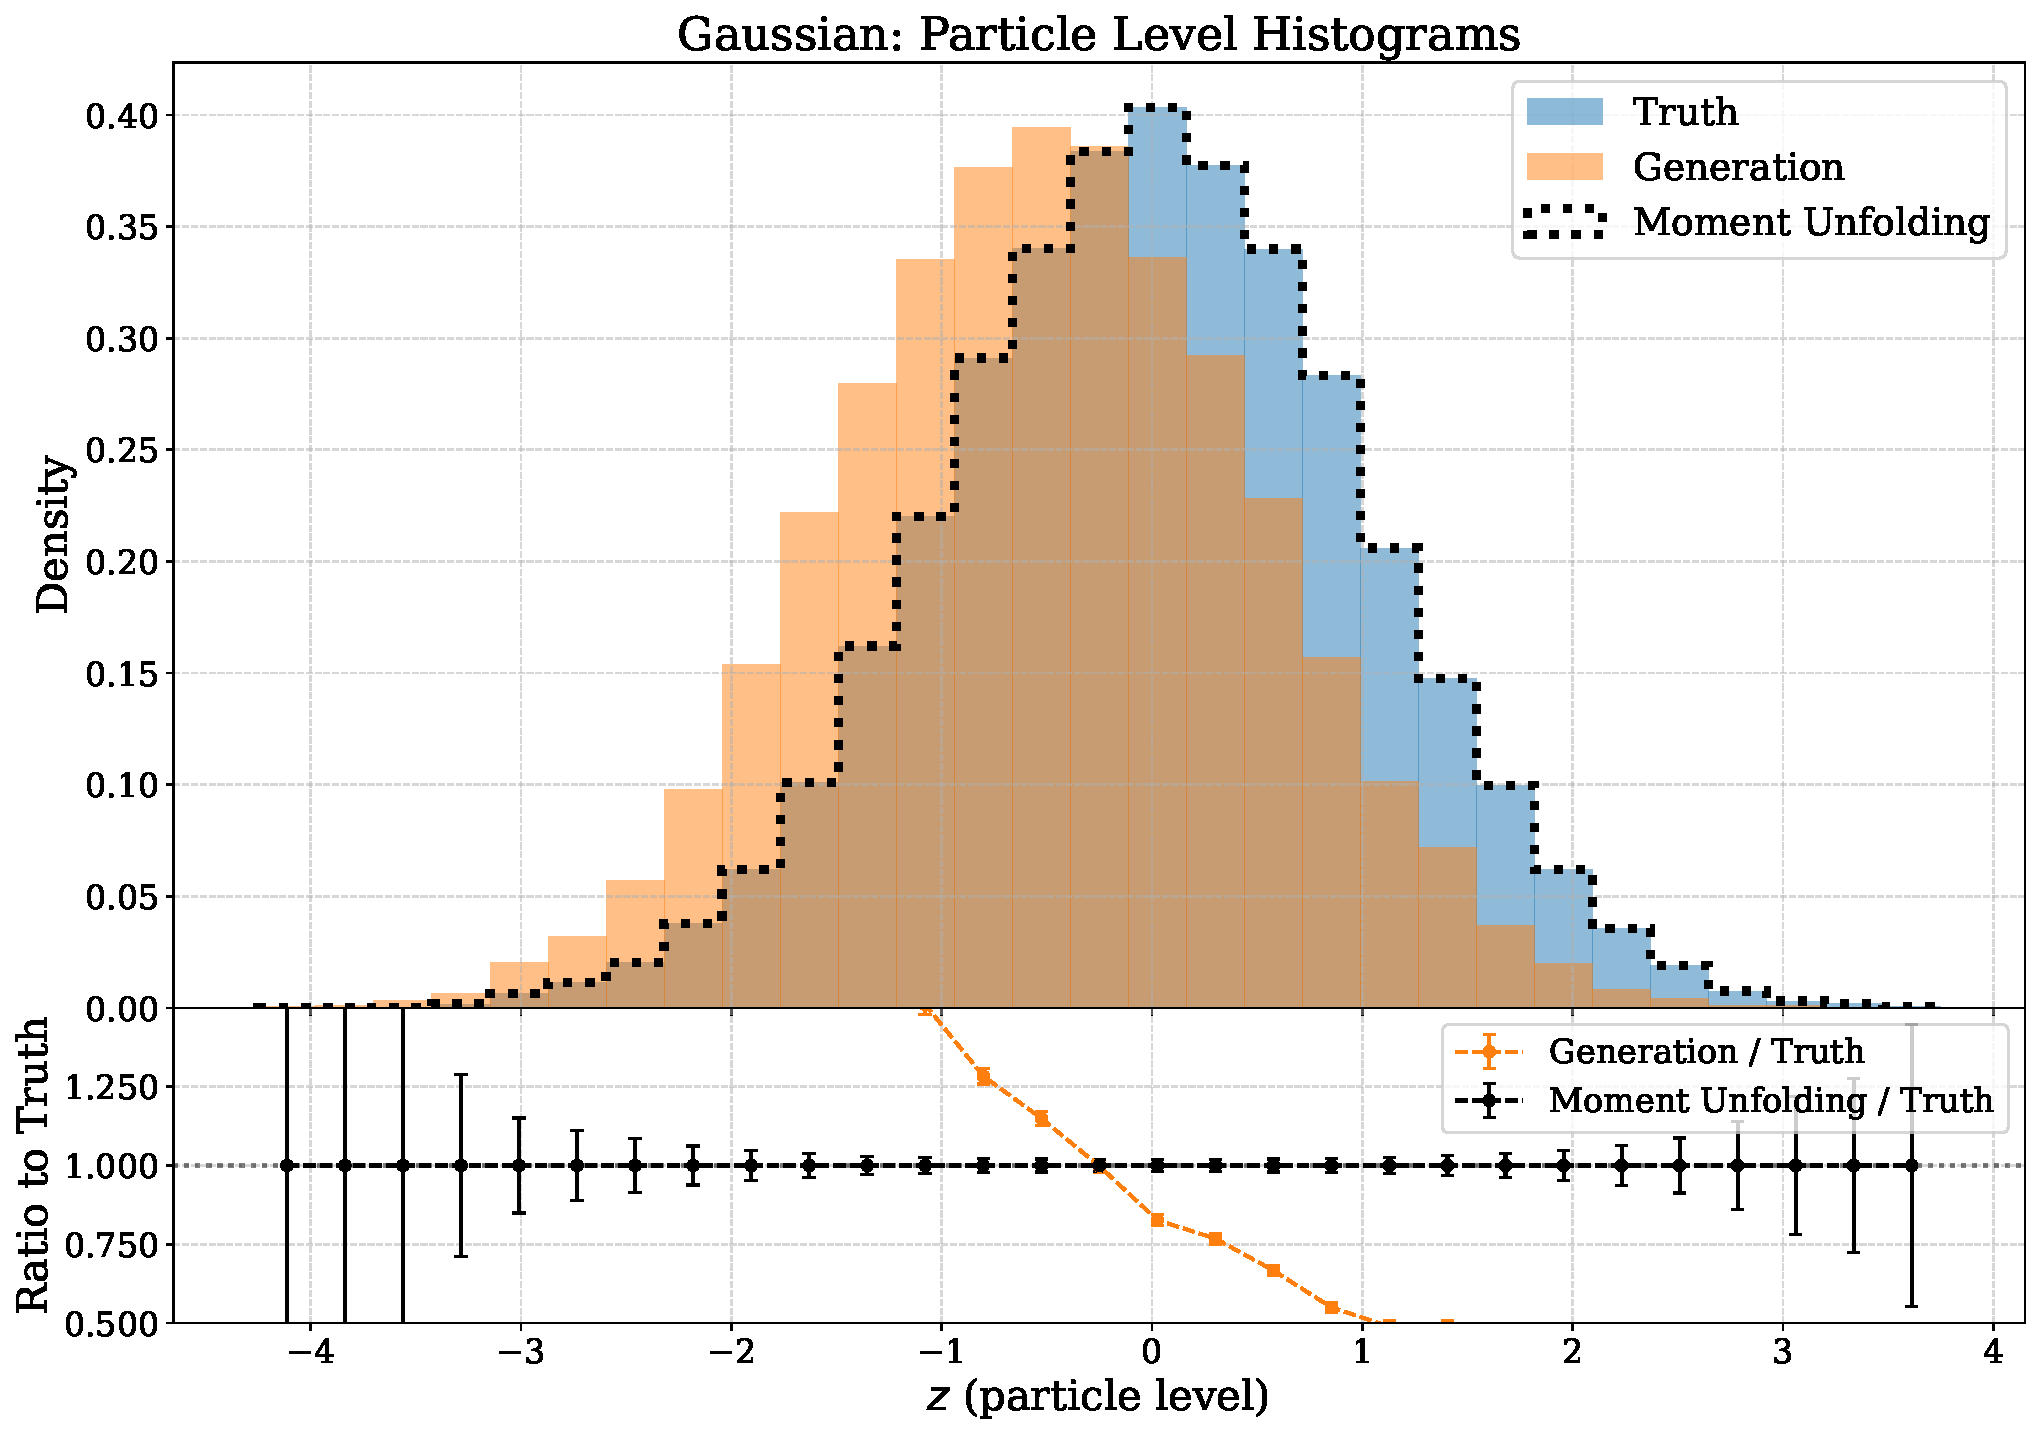
\includegraphics[height=0.38\textwidth]{figures/chapter-05/gaussexample.pdf}
    \label{fig:gaussexample}}
    \subfloat[]{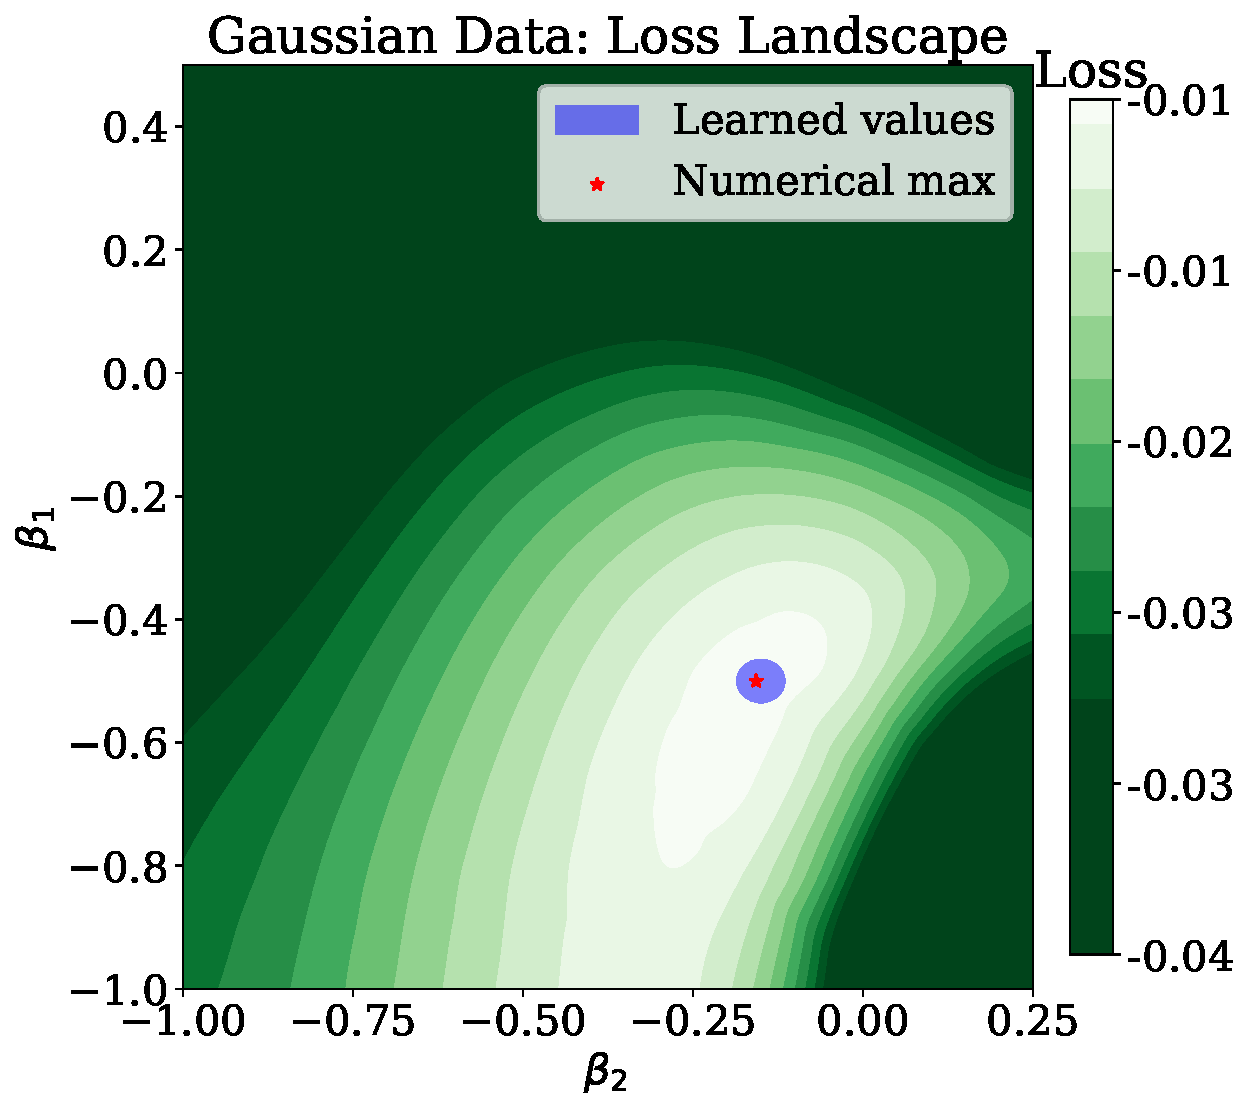
\includegraphics[height=0.38\textwidth]{figures/chapter-05/gaussloss.pdf}
        \label{fig:gaussloss}}
    \caption{
    %
    (a) Distributions from the Gaussian example of particle level truth, generation, and reweighted generation i.e.~\textsc{Moment Unfolding}.
    %
    The agreement between the truth and reweighted samples demonstrates the qualitative performance of \textsc{Moment Unfolding}.
    %
    (b) The weighted MLC loss from \cref{eq:numericloss} for fixed $g$ but optimized $d$, found by scanning over $\beta_1$ and $\beta_2$.
    %
    The correct value is indicated by a red star.
    %
    Indicated in shaded blue is the $1\sigma$ bootstrapped interval for \textsc{Moment Unfolding}'s prediction of $\beta_a$.The lower panel in each plot shows the ratio to truth.
    }
        \label{fig:gauss}
\end{figure}
    \subsection{Jet substructure in collider physics}
    \label{subsec:jet-moments}
        Having validated \textsc{Moment Unfolding} in a controlled environment, we now apply the method to a realistic high energy physics scenario: measuring moments of jet substructure observables in simulated proton--proton collisions at the Large Hadron Collider (LHC).
        \subsubsection{Datasets}
            The simulated samples used for this study follow the setup from~\cite{andreassen_omnifold_2020}.
            %
            Proton--proton collisions at $\sqrt{s} = 14$ TeV are simulated using \textsc{Pythia 8.243} with Tune 26 (standing in for MC) and \textsc{Herwig 7.1.5} (standing in for nature).
            %
            The \textsc{Delphes 3.4.2} fast simulation of the CMS detector is used to model detector effects, configured with particle flow reconstruction.
            %
            Jets are clustered using the anti-$k_T$ algorithm with radius parameter $R = 0.4$, implemented in \textsc{FastJet 3.3.2}.
            %
            To reduce acceptance effects, only leading jets in events with a Z boson having transverse momentum $p_T^Z > 200$ GeV are included.
            %
            This setup allows us to test \textsc{Moment Unfolding} in a realistic environment where the ``Truth'' (\textsc{Herwig} particle level) and ``Generation" (\textsc{Pythia} particle level) are different generators with distinct physics models, and both are observed through an imperfect detector to produce ``Data'', \textsc{Herwig + Delphes} and ``Simulation'', \textsc{Pythia + Delphes}.
            \subsubsection{Observables}
                Four key jet substructure observables are unfolded, each providing different insights into the internal structure of jets.
                \begin{enumerate}
                \item \textbf{Jet mass} ($m$): The invariant mass of the jet, calculated as
                \[
                    m = \sqrt{\sum_k E_k^2 - \sum_k \mathbf{p}_k^2},
                \]
                where the sum runs over all constituents of the jet, and $E_k$ and $\mathbf{p}_k$ are their energies and \(3-\)momenta.
            \item \textbf{Jet charge} ($q$): An infrared--safe but not collinear--safe observable that measures the jet's electric charge~\cite{Kang:2023ptt, ATLAS:2015rlw}.
            \[
                q = \frac{1}{\sum_k \sqrt{p_{T,k}}}\sum_k q_k \sqrt{p_{T,k}},
            \]
            where $q_k$ is the electric charge of constituent $k$.
            %
            On account of being non collinear safe, jet expected to be more susceptible to certain kinds of detector distortions.
            %
            The first moment of the jet charge distribution as a function of jet $p_T$ has been calculated in~\cite{Krohn2013JetLHC,Waalewijn2012CalculatingJet,Li:2019dre,Li2020JetMatter,Kang2020JetCollider} and measured by ATLAS~\cite{ATLAS:2015rlw} and CMS~\cite{CMS:2017yer,CMS:2020plq}.
            \item \textbf{Jet width} ($w$): A measure of the radial distribution of radiation within the jet.
            \[
                w = \frac{1}{p_{T,\text{jet}}}\sum_k p_{T,k} \Delta R_k,
            \]
            where $\Delta R_k$ is the angular distance between constituent $k$ and the jet axis.
            \item \textbf{Groomed momentum fraction} ($z_g$)~\cite{Larkoski:2015lea}: The momentum sharing between subjets after Soft Drop grooming~\cite{Dasgupta2013TowardsSubstructure, Larkoski2014SoftDrop} with $z_{\text{cut}} = 0.1$ and $\beta = 0$.
            \[
                z_g = \frac{p_{T,\text{subleading}}}{p_{T,\text{leading}} + p_{T,\text{subleading}}}
            \]
            where \(p_{T,\text{leading}}\) and \(p_{T,\text{subleading}}\) refer to transverse momentum of the leading and subleading prongs respectively~\cite{ALargeIonColliderExperiment:2021mqf}
            \end{enumerate}
            These observables span a diverse range of jet properties, including both infrared and collinear safe observables ($m$ and $w$), a Sudakov safe observable, \(z_g\), and \(q\), which is only infrared safe.
\subsubsection{Results}
            \begin{table}
              \centering
              \label{tab:inclusive-moments}
              \caption{
                  Moments of jet observables at particle level.
                  %
                  First and second moments of \(m, q, w\) and \(z_g\) are shown for truth (\textsc{Herwig}), generation (\textsc{Pythia}) and Moment Unfolding.
                  %
                  Uncertainties in the truth and generation columns are estimated via bootstrap resampling; uncertainties in the unfolding column combine in quadrature the generation bootstrap uncertainty with the empirical \(1\sigma\) spread from repeated unfolding on the same dataset.
              }
              \begin{tabular}{|c|c|c|c|}
                \hline
                              & Truth (\textsc{Herwig})                   & Generation (\textsc{Pythia})               & Moment Unfolding                  \\
                \hline
                \hline
                $\langle m \rangle$   & $(2.182 \pm 0.030)\times10^{1}$   & $(2.064 \pm 0.043)\times10^{1}$   & $(2.173 \pm 0.047)\times10^{1}$   \\
                $\langle m^2 \rangle$ & $(6.049 \pm 0.222)\times10^{2}$   & $(5.360 \pm 0.350)\times10^{2}$   & $(6.115 \pm 0.364)\times10^{2}$   \\
                \hline
                $\langle q \rangle$   & $(1.006 \pm 0.037)\times10^{-2}$  & $(1.582 \pm 0.038)\times10^{-2}$  & $(1.090 \pm 0.040)\times10^{-2}$  \\
                $\langle q^2 \rangle$ & $(1.216 \pm 0.082)\times10^{-2}$  & $(1.508 \pm 0.074)\times10^{-2}$  & $(1.207 \pm 0.074)\times10^{-2}$  \\
                \hline
                $\langle w \rangle$   & $(1.498 \pm 0.025)\times10^{-1}$  & $(1.231 \pm 0.029)\times10^{-1}$  & $(1.499 \pm 0.029)\times10^{-1}$  \\
                $\langle w^2 \rangle$ & $(3.370 \pm 0.113)\times10^{-2}$  & $(2.421 \pm 0.128)\times10^{-2}$  & $(3.374 \pm 0.128)\times10^{-2}$  \\
                \hline
                $\langle z_g \rangle$ & $(2.334 \pm 0.029)\times10^{-1}$  & $(2.457 \pm 0.030)\times10^{-1}$  & $(2.353 \pm 0.059)\times10^{-1}$  \\
                $\langle z_g^2 \rangle$ & $(6.789 \pm 0.166)\times10^{-2}$ & $(7.425 \pm 0.165)\times10^{-2}$  & $(6.767 \pm 0.330)\times10^{-2}$  \\
                \hline
              \end{tabular}
            \end{table}
            \cref{tab:inclusive-moments} presents the first and second moments of each jet observable extracted using \textsc{Moment Unfolding}, compared with the true values (from \textsc{Herwig}) and those from the generation (\textsc{Pythia}) in tabular form.
            %
            The uncertainties in the Truth and Generation columns are computed by bootstrapping the respective datasets.
            %
            For the \textsc{Moment Unfolding} column, the uncertainty includes the bootstrap uncertainty from the Generation and the empirical uncertainty from the unfolding process added in quadrature.
            %
            The empirical uncertainty from the unfolding process is computed by repeating \textsc{Moment Unfolding} on the same data and computing the \(1\sigma\) spread
            
            These results demonstrate that \textsc{Moment Unfolding} successfully recovers the true moments from the data for all observables within statistical uncertainties.
            %
            The method effectively corrects for both the differences between the \textsc{Pythia} and \textsc{Herwig} physics models and the detector distortions introduced by \textsc{Delphes}.

            \cref{fig:jetexample_dists} shows the particle level distributions for each observable, comparing the truth, generation, and reweighted generation after applying \textsc{Moment Unfolding}
            %
            While the method explicitly targets only the first two moments, it produces reasonable agreement across the entire distribution, particularly for the regions that contribute most significantly to the moments.

\begin{figure}
\subfloat[]{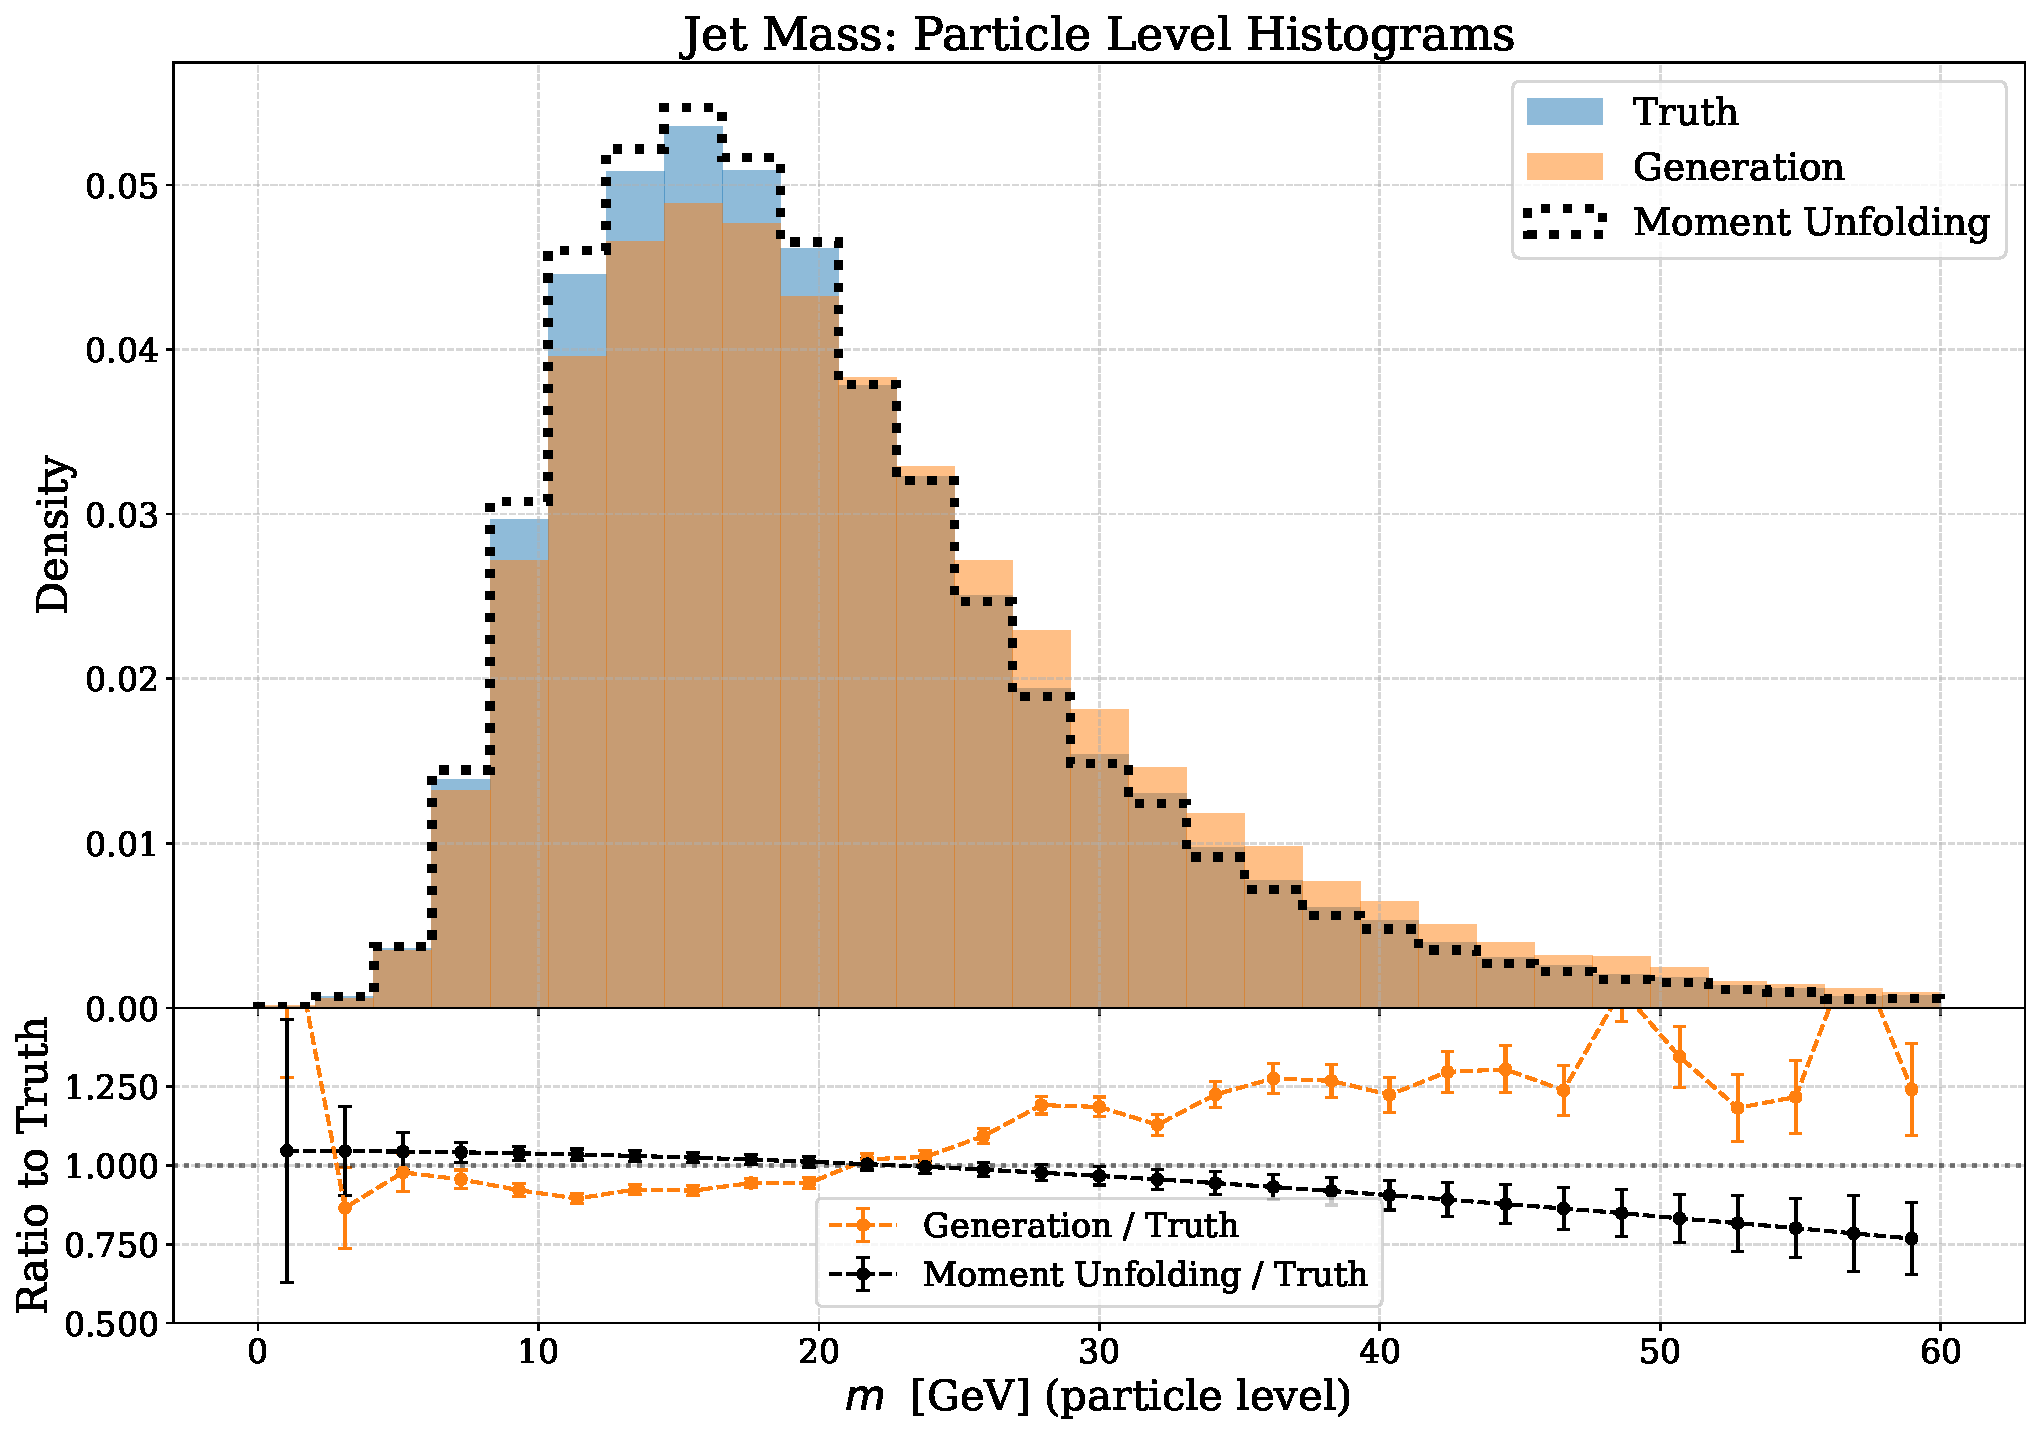
\includegraphics[height=0.32\textwidth]{figures/chapter-05/mjetexample.pdf}}
\subfloat[]{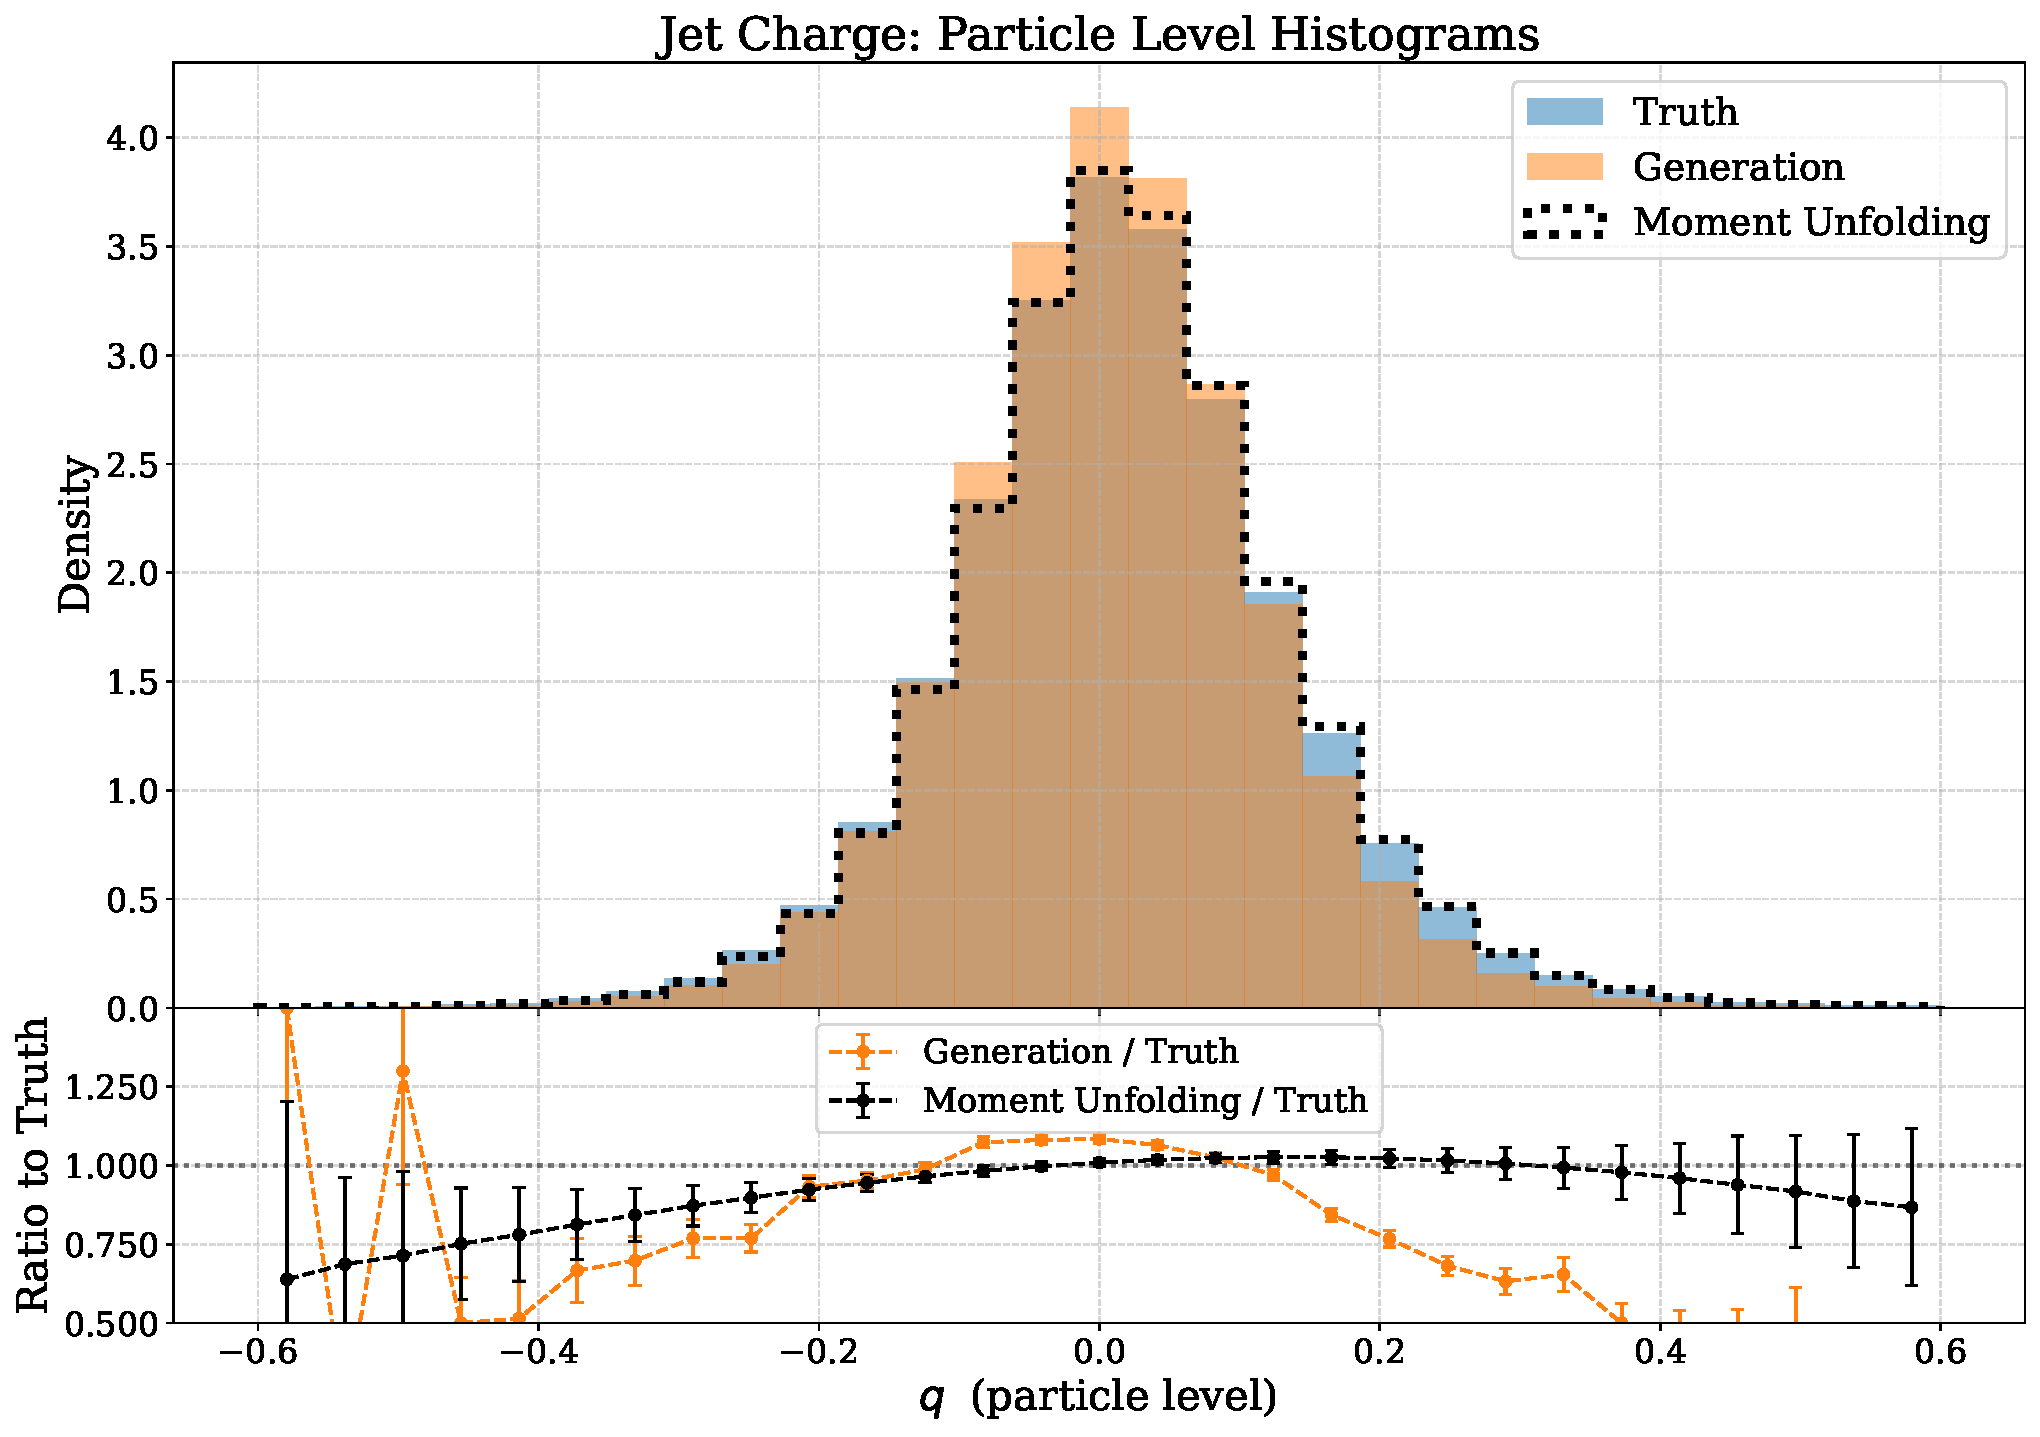
\includegraphics[height=0.32\textwidth]{figures/chapter-05/qjetexample.pdf}}\\
\subfloat[]{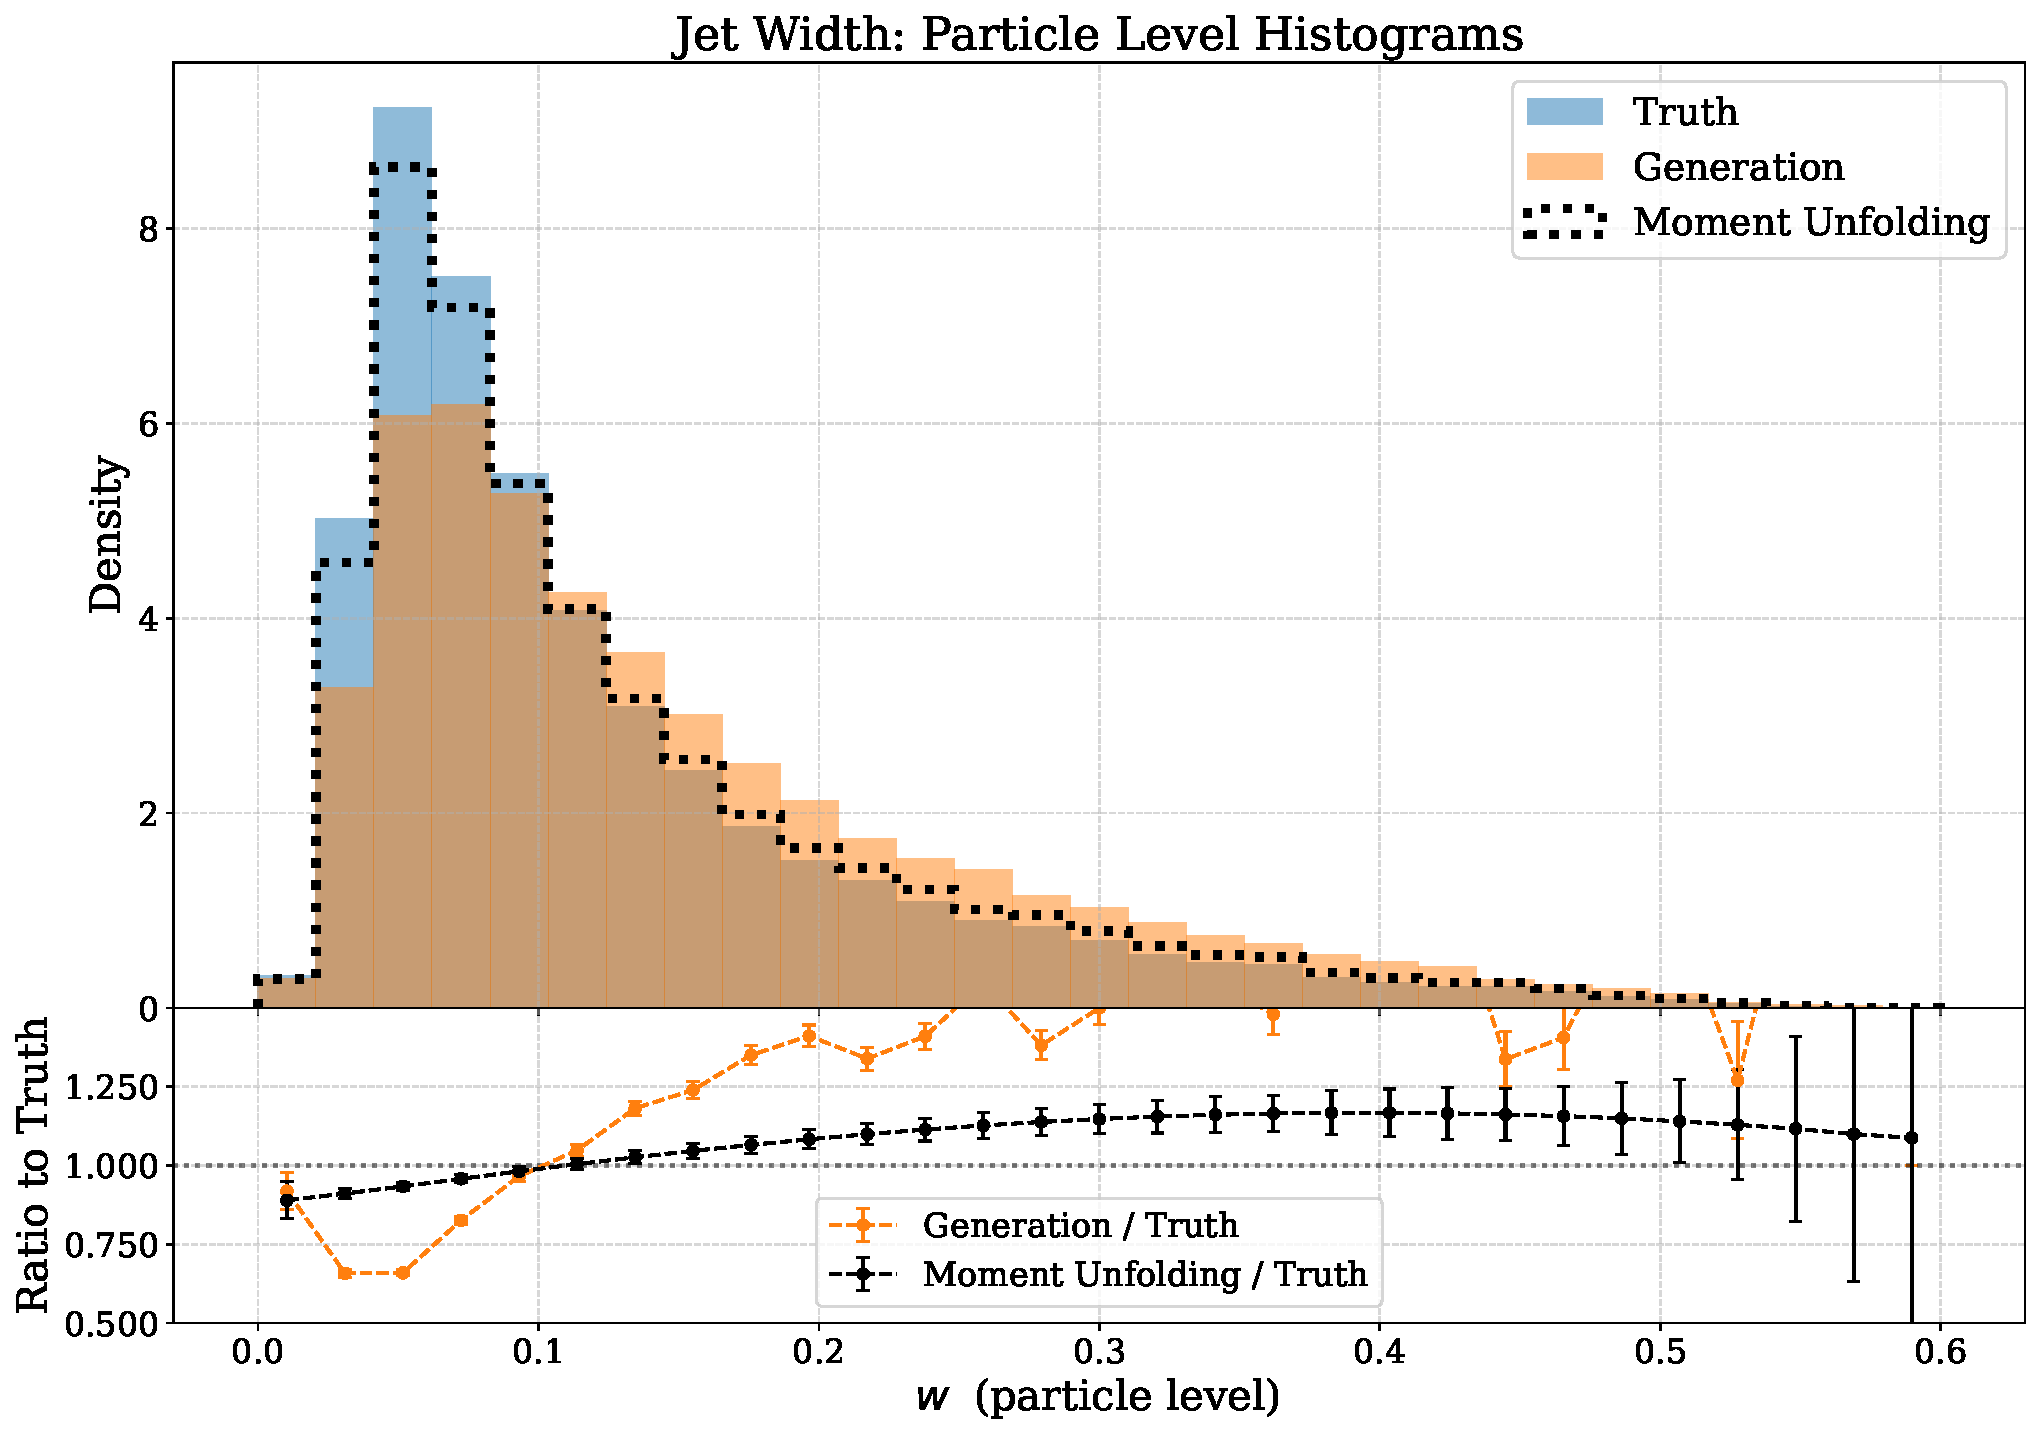
\includegraphics[height=0.32\textwidth]{figures/chapter-05/wjetexample.pdf}}
\subfloat[]{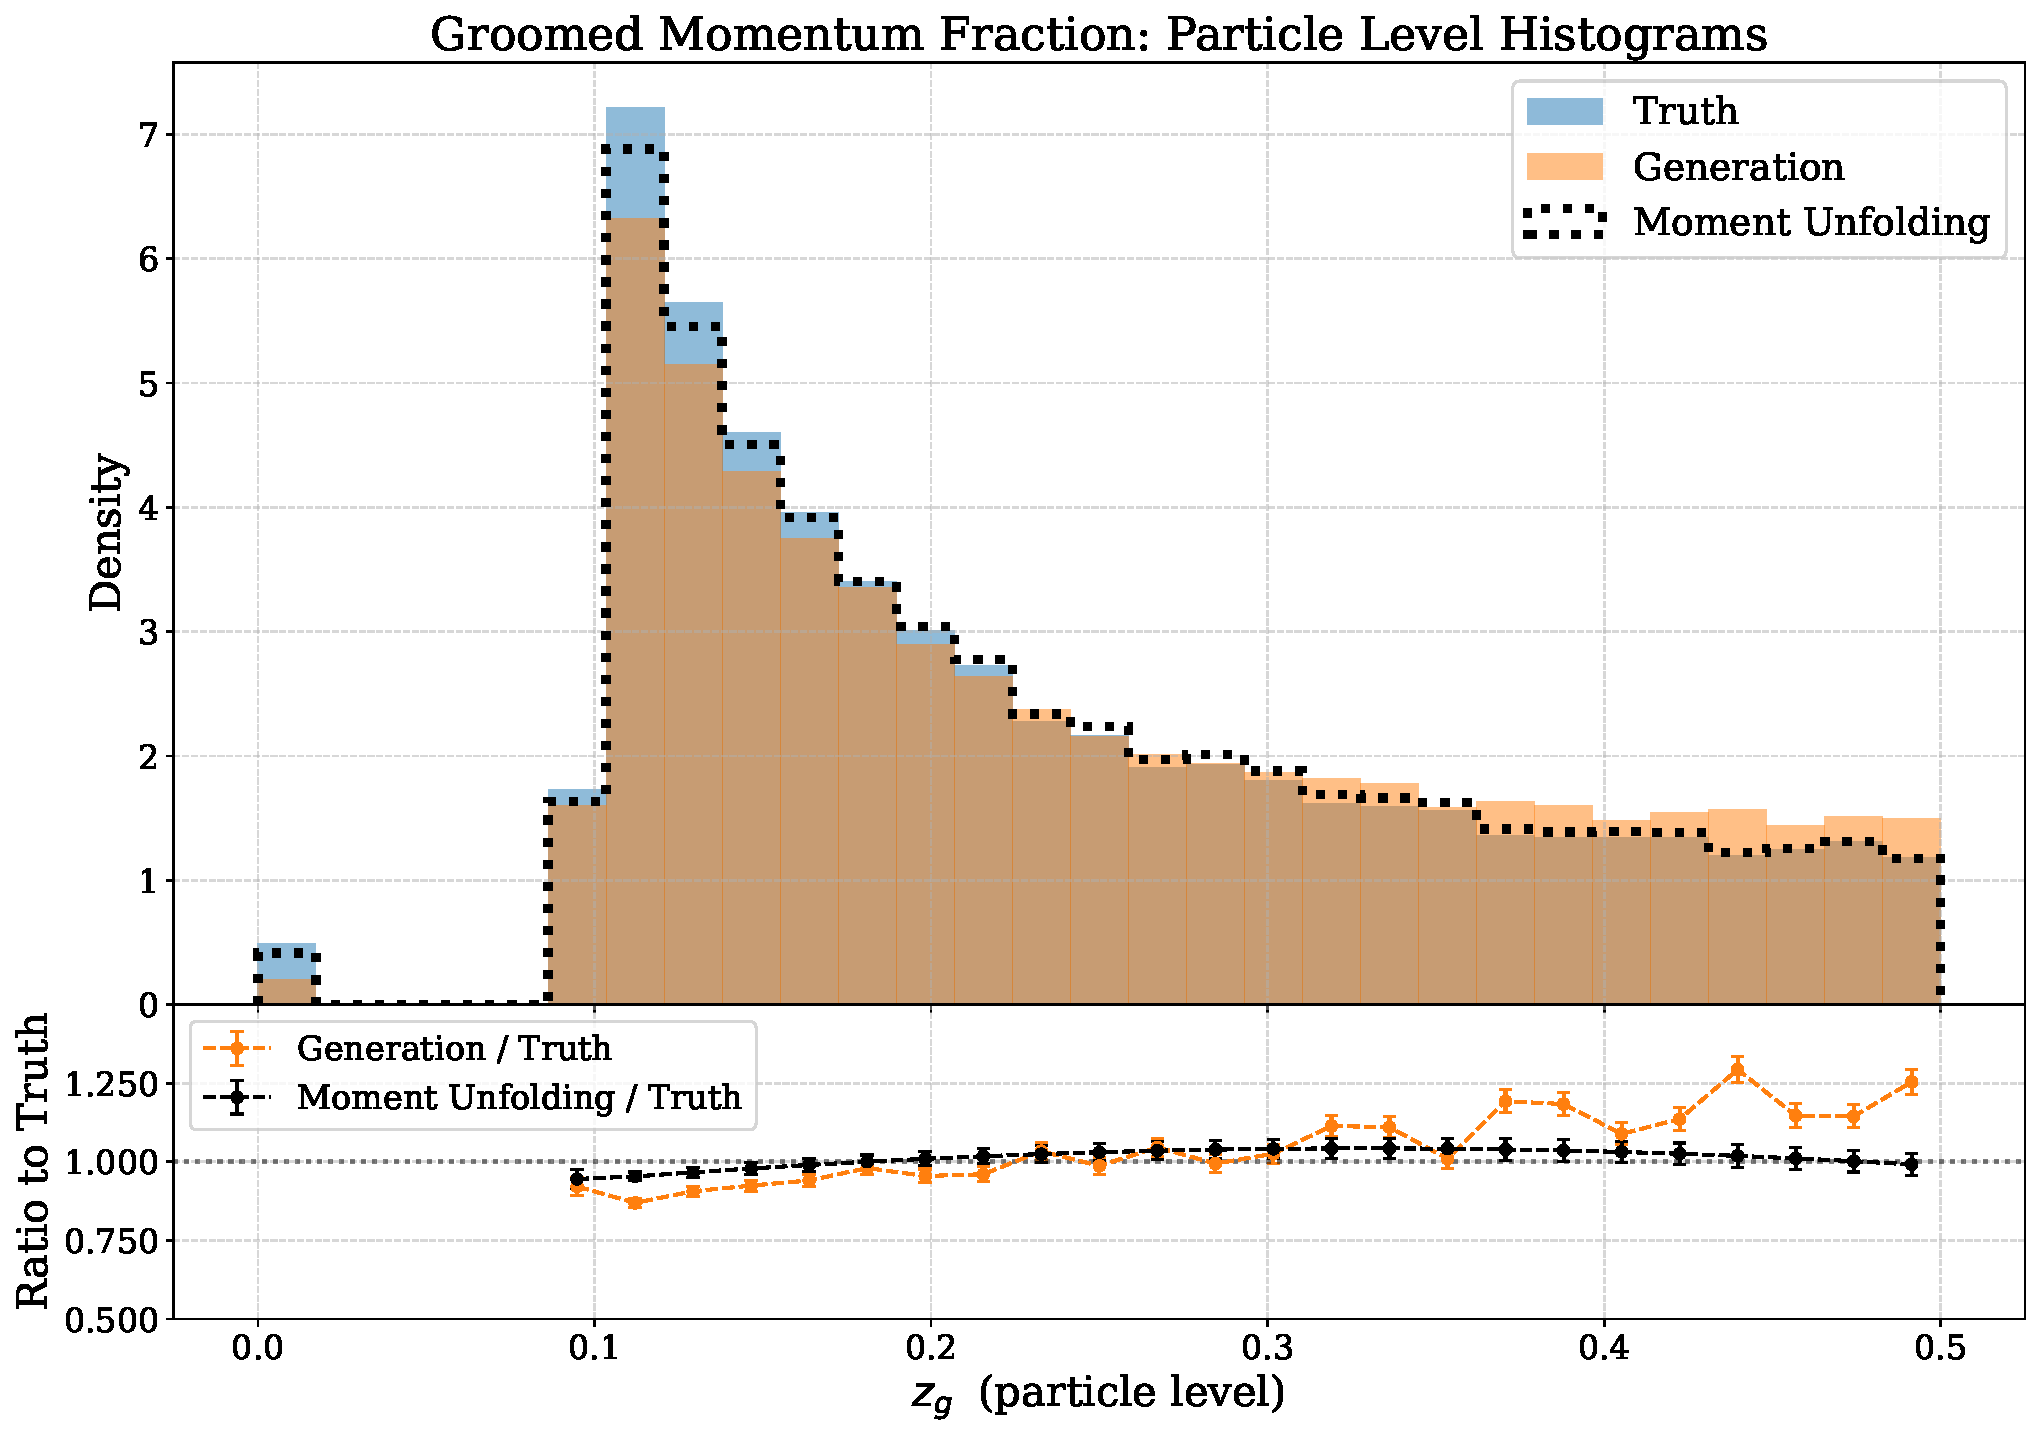
\includegraphics[height=0.32\textwidth]{figures/chapter-05/zgjetexample.pdf}}
\caption[Jet substructure distributions comparing truth, generation, and \textsc{Moment Unfolding} results]{Distributions of (a) jet mass, (b) jet charge, (c) jet width, and (d) groomed momentum fraction at particle level for leading jets in $Z$+jet events at $\sqrt{s} = 14$ TeV. The plots compare Truth (\textsc{Herwig}), Generation (\textsc{Pythia}), and reweighted Generation after applying \textsc{Moment Unfolding} weights to correct Generation.
%
The \textsc{Moment Unfolding} method successfully adjusts the generated distributions to match the truth, demonstrating effective correction across all four jet substructure observables. The lower panel in each plot shows the ratio to truth.}
\label{fig:jetexample_dists}
\end{figure}
            \cref{fig:jetexample_loss} displays the discriminator optimised loss landscapes for each observable, confirming that the maximum of the loss function aligns with the parameter values that produce the correct moments.
            %
            The blue ellipses represent the \(1\sigma\) confidence intervals for the \textsc{Moment Unfolding} parameters, and they all contain the true parameter values (red dots), indicating proper uncertainty estimation.
\begin{figure}
    \subfloat[]{ 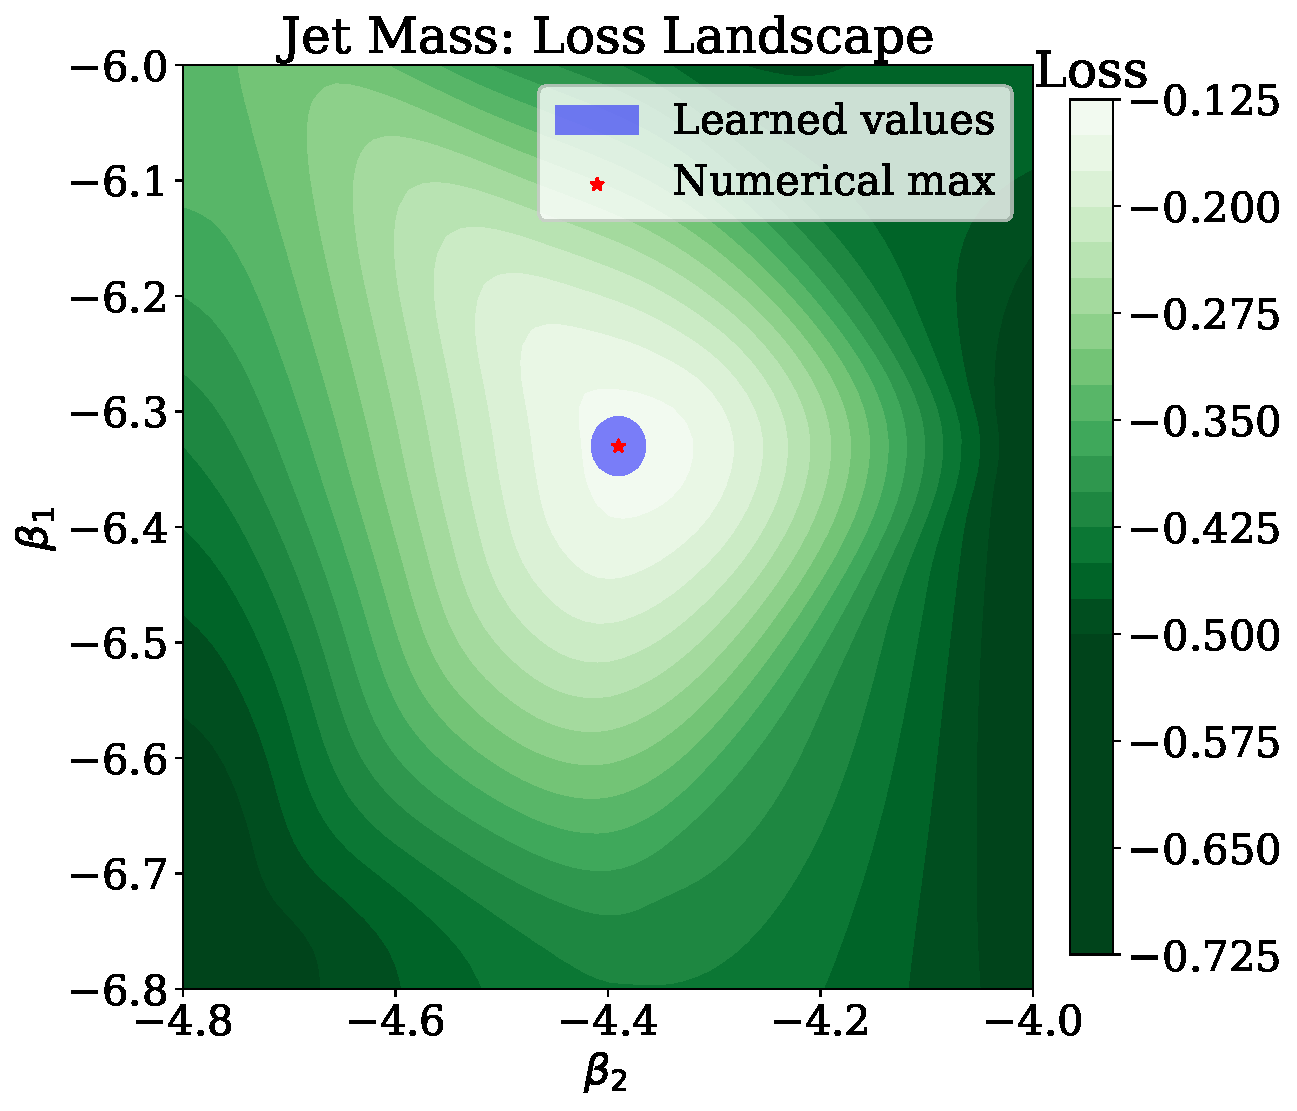
\includegraphics[height=0.4\textwidth]{figures/chapter-05/mjetloss.pdf}\label{fig:mjetloss}}
    \subfloat[]{ 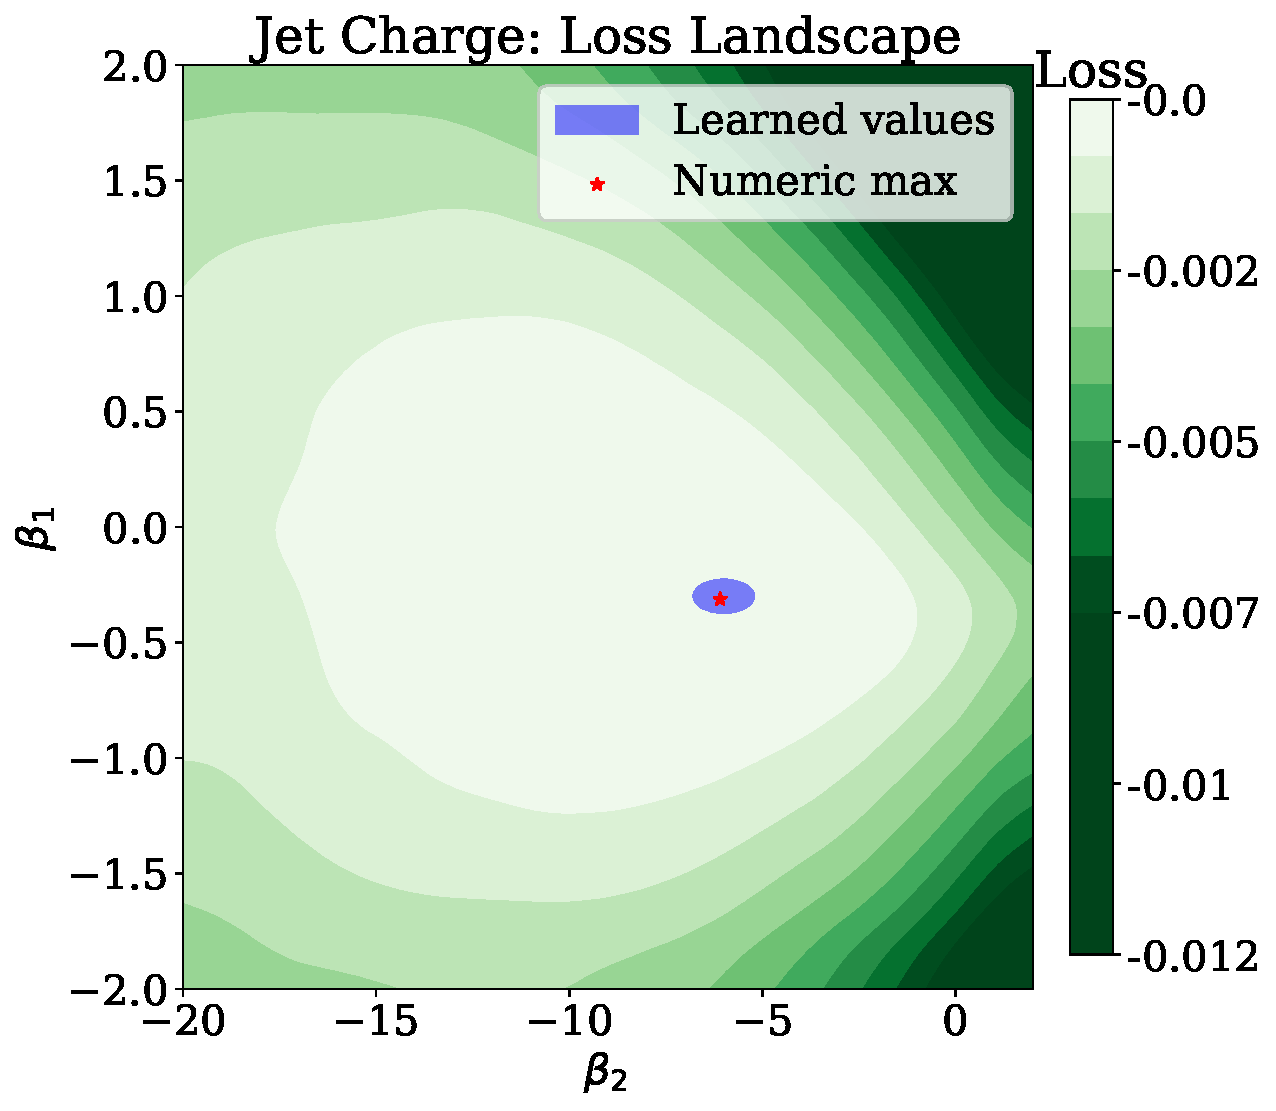
\includegraphics[height=0.4\textwidth]{figures/chapter-05/qjetloss.pdf}\label{fig:qjetloss}}\\
    
    \subfloat[]{ 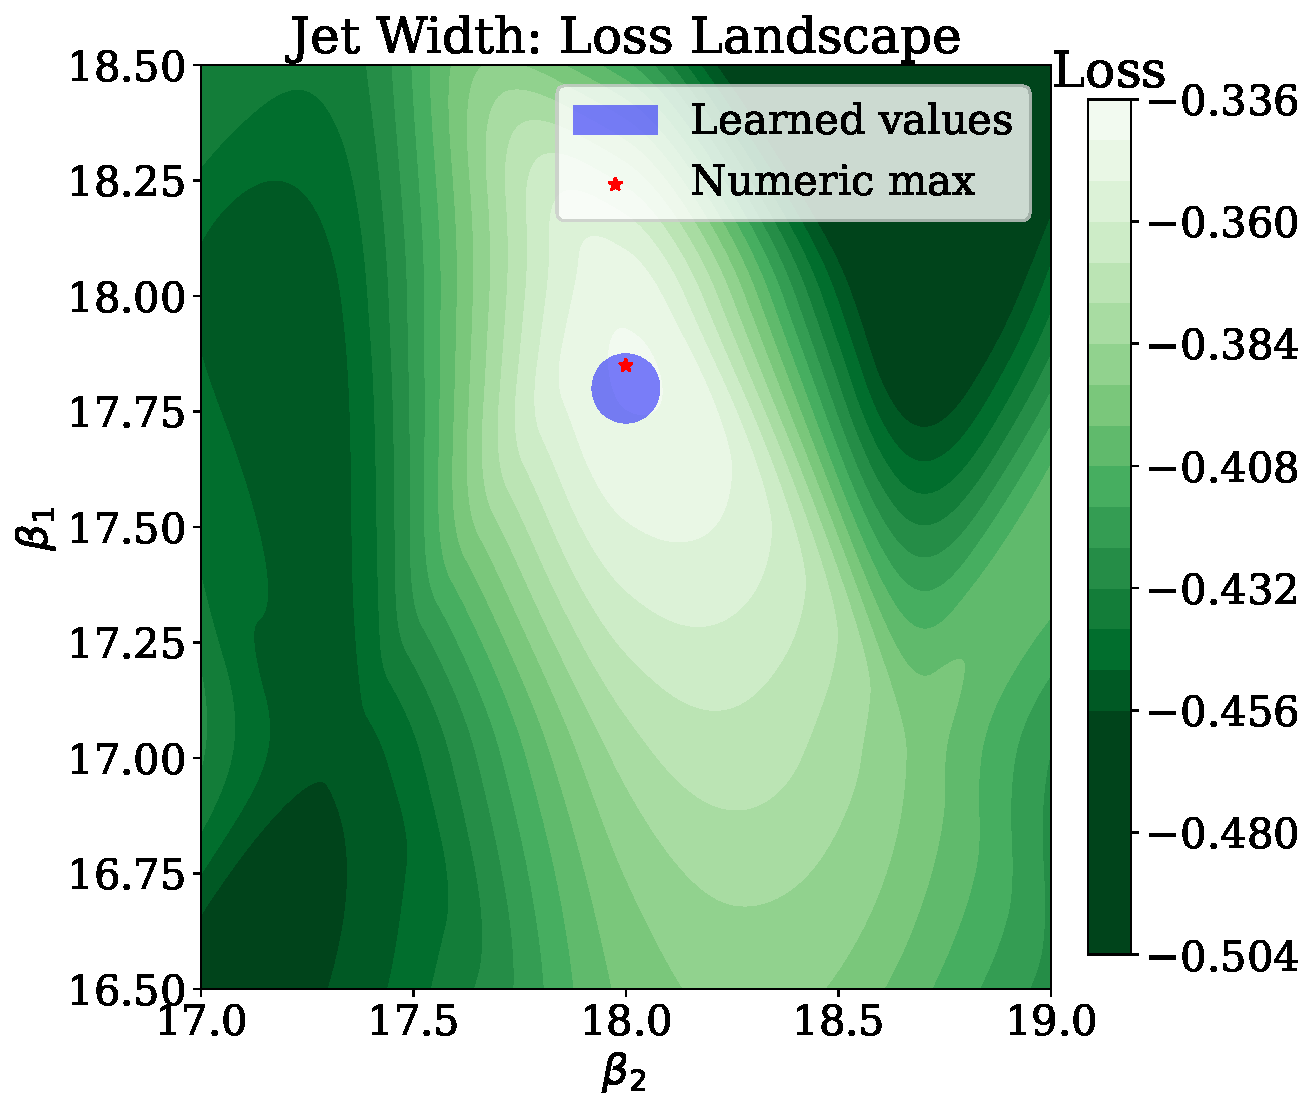
\includegraphics[height=0.4\textwidth]{figures/chapter-05/wjetloss.pdf}\label{fig:wjetloss}}
    \subfloat[]{ 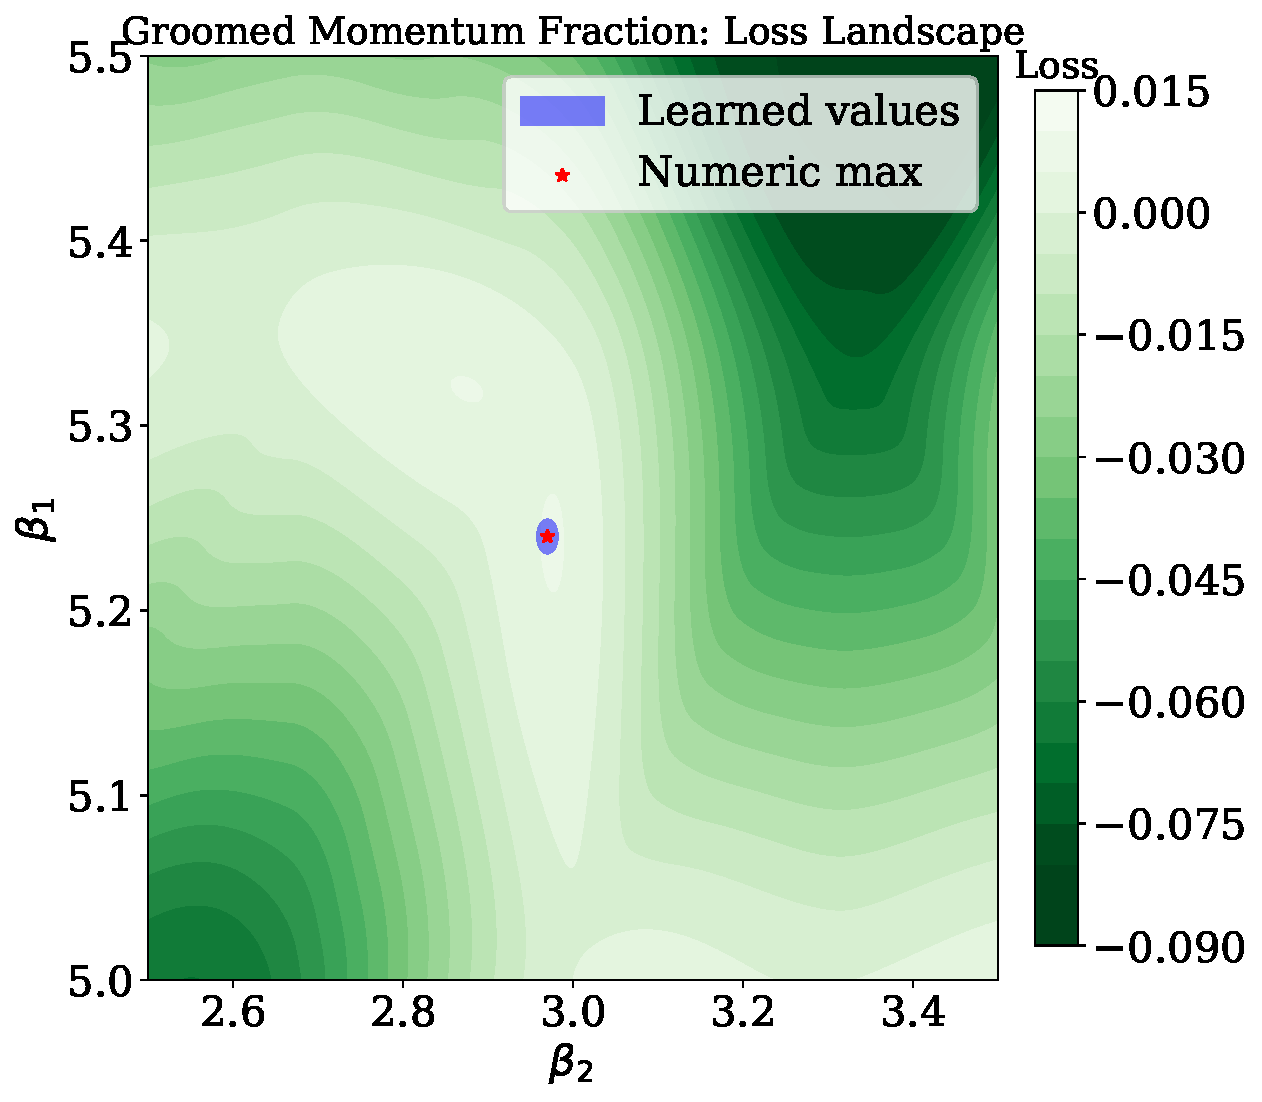
\includegraphics[height=0.4\textwidth]{figures/chapter-05/zgjetloss.pdf}\label{fig:zgjetloss}}
\caption[Loss landscapes showing \textsc{Moment Unfolding} parameter estimation accuracy for unfolding jet substructure variable.]{The discriminator-optimized Maximum Likelihood Classifier (MLC) loss landscapes as a function of the \textsc{Moment Unfolding} parameters $\beta_1$ and $\beta_2$ for (a) jet mass, (b) jet charge, (c) jet width, and (d) groomed momentum fraction. The true parameter values that correctly map between the generation and truth distributions are indicated by red dots, while the $1\sigma$ confidence intervals from \textsc{Moment Unfolding}'s parameter estimation are shown as blue ellipses. The alignment of the loss function maxima with the true parameter values and the containment of these values within the uncertainty ellipses demonstrates both the accuracy of the method and the reliability of its uncertainty estimation.}
    \label{fig:jetexample_loss}
\end{figure}
    
    \subsection{Momentum dependent unfolding}
        One of the most powerful features of \textsc{Moment Unfolding} is its ability to extract moments as a function of another observable, such as jet transverse momentum.
        %
        When implemented with momentum--dependent parameters in the Boltzmann weight function, the generator described in \cref{eq:pt-moment-gen} unfolds moments conditional on the jet \(p_T\).
        
        This ability to unfold moments as functions of \(p_T\) is a necessary feature for any modern unfolding method.
        %
        Many QCD phenomena exhibit strong scale dependence, including parton shower evolution, hadronization effects, and detector response.
        %
        Understanding the momentum dependence is necessary to account for these variations.
        
        Jets at different \(p_T\) values populate different regions of the substructure phase space.
        %
        A momentum dependent reweighting is therefore important for better coverage of the phase space.
        %
        The momentum dependent approach effectively leverages the statistical power of the entire dataset while allowing for local adaptations in different \(p_T\) regions, resulting in more precise measurements overall.

        The implementation of momentum dependent parameters, \(\beta_a(p_T)\) introduces additional complexity that must be carefully managed.
        
        For this data, a linear parametrisation of \(\beta_a(p_T)\) provides a good balance between flexibility and stability for the jet substructure observables studied.\footnote{\textsc{Moment Unfolding} can be run as a binned method by parametrising \(\beta_a(p_T)\) as a piecewise constant function.}
        %
        More complex parametrisations might be warranted for observables with a strongly non-linear \(p_T\) dependence.
        %
        However, increasing the number of parameters in the momentum dependent approach must be approached with caution, since that, in some ways, lifts the regularisation imposed by the \textsc{Moment Unfolding} method.
        %
        If the training remains unstable despite appropriately constraining the functional form of \(\beta_a(p_T)\) regularisation in the neural network training may become necessary.
        %
        Some successful approaches to regularise such neural network trainings can be found in \cref{subsec:regularisation-in-ran}.
        
        \subsubsection{Inclusive distributions.}
            \cref{fig:pjetexample} presents the inclusive distributions of jet mass, jet charge, jet width, and groomed momentum fraction after applying momentum dependent \textsc{Moment Unfolding}.
            %
            Compared to the non-momentum dependent results shown in \cref{fig:jetexample_dists}, these distributions demonstrate markedly better agreement with the truth.
            %
            This improvement occurs because the momentum dependent approach effectively implements a more refined correction, allowing the reweighting function to adapt to the changing detector response and physics differences across the \(p_T\) spectrum.
            %
            By parametrising \(\beta_a\) as a function of \(p_T\), we account for the fact that both detector effects and physics modelling discrepancies can vary significantly with jet energy.

            The inclusive distributions obtained through momentum conditioned unfolding also reveal subtle physical features that might be obscured in the non--conditioned approach.
            %
            For example, in the jet mass distribution, the shape of the low mass region shows better agreement with truth when using momentum conditioning, correctly capturing the interplay between soft radiation and resolution effects that varies with jet \(p_T\).

\begin{figure}
    \centering
    \subfloat[]{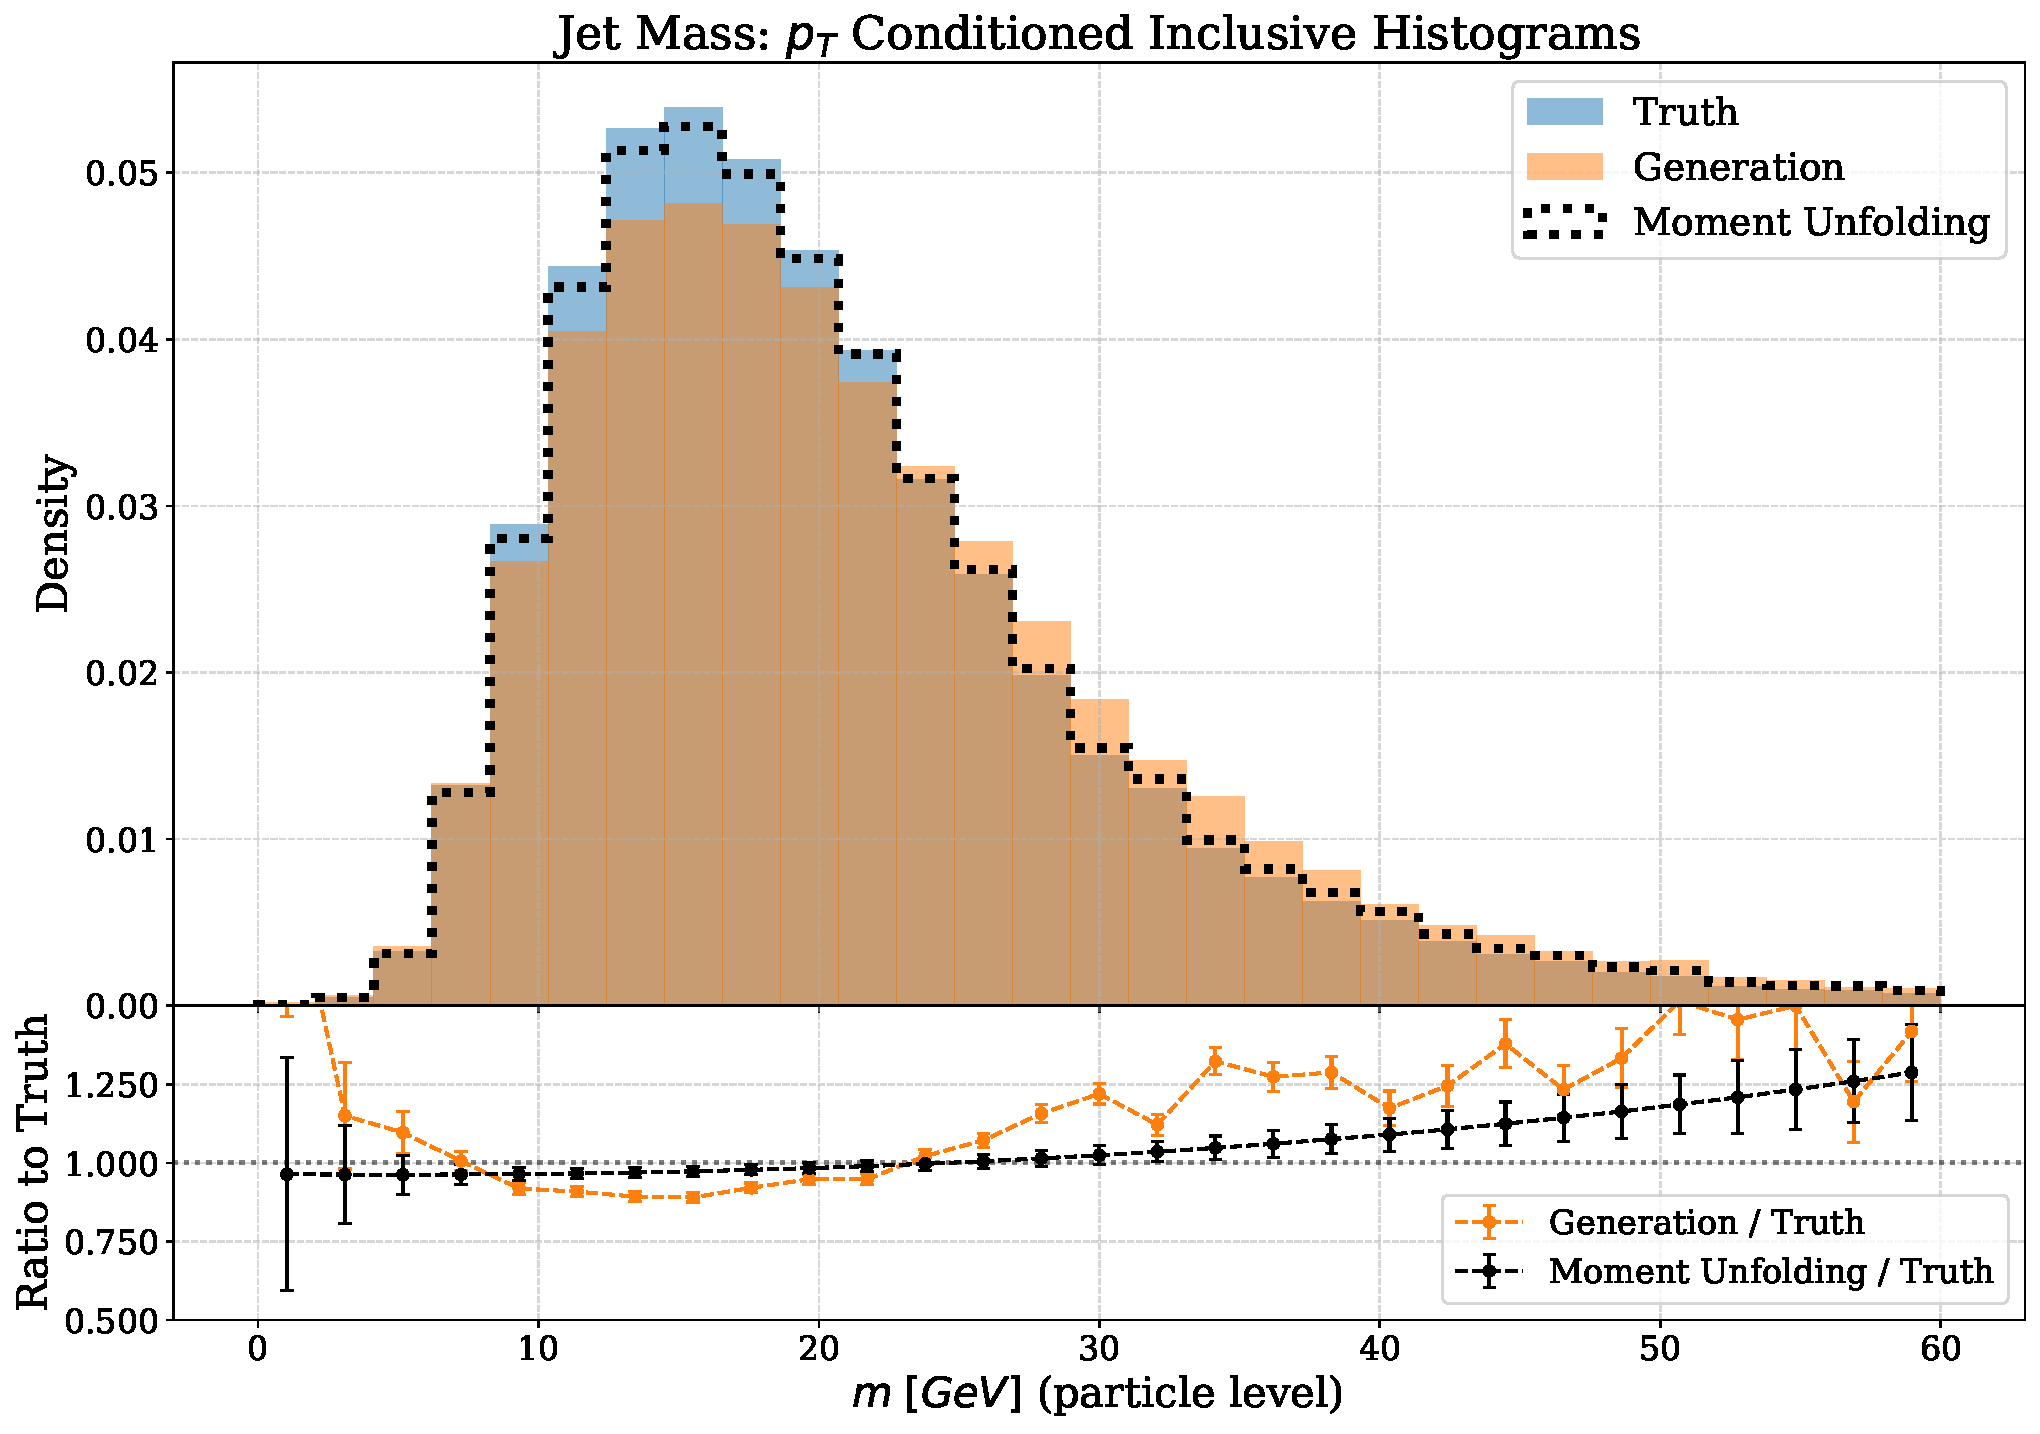
\includegraphics[height=0.32\textwidth]{figures/chapter-05/mpjetexample.pdf}}
    \subfloat[]{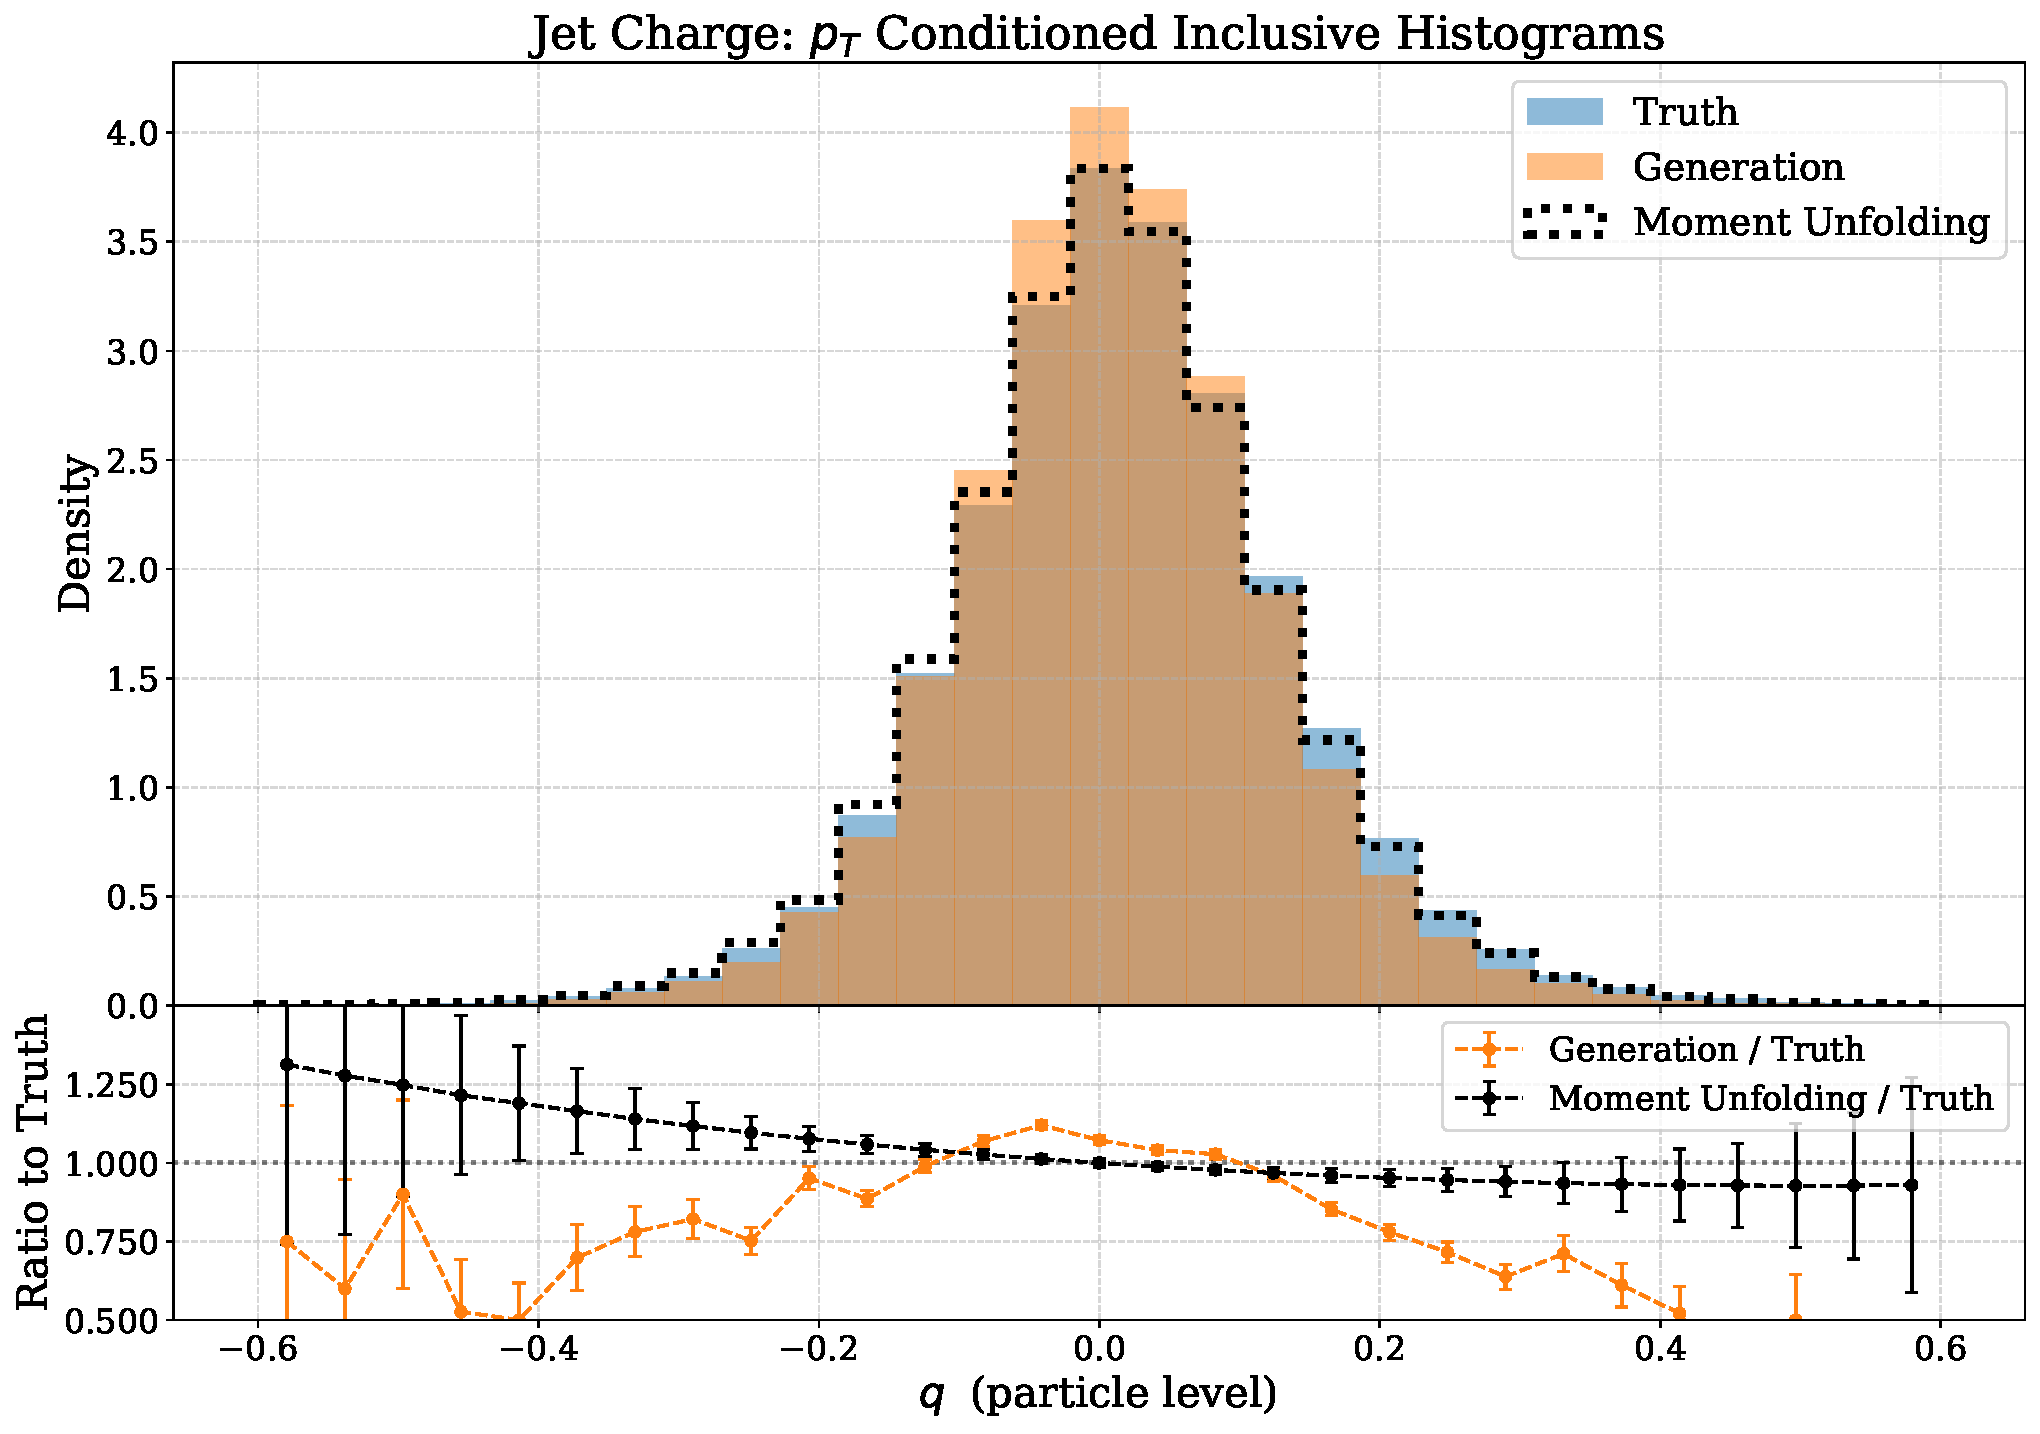
\includegraphics[height=0.32\textwidth]{figures/chapter-05/qpjetexample.pdf}}\\
    \subfloat[]{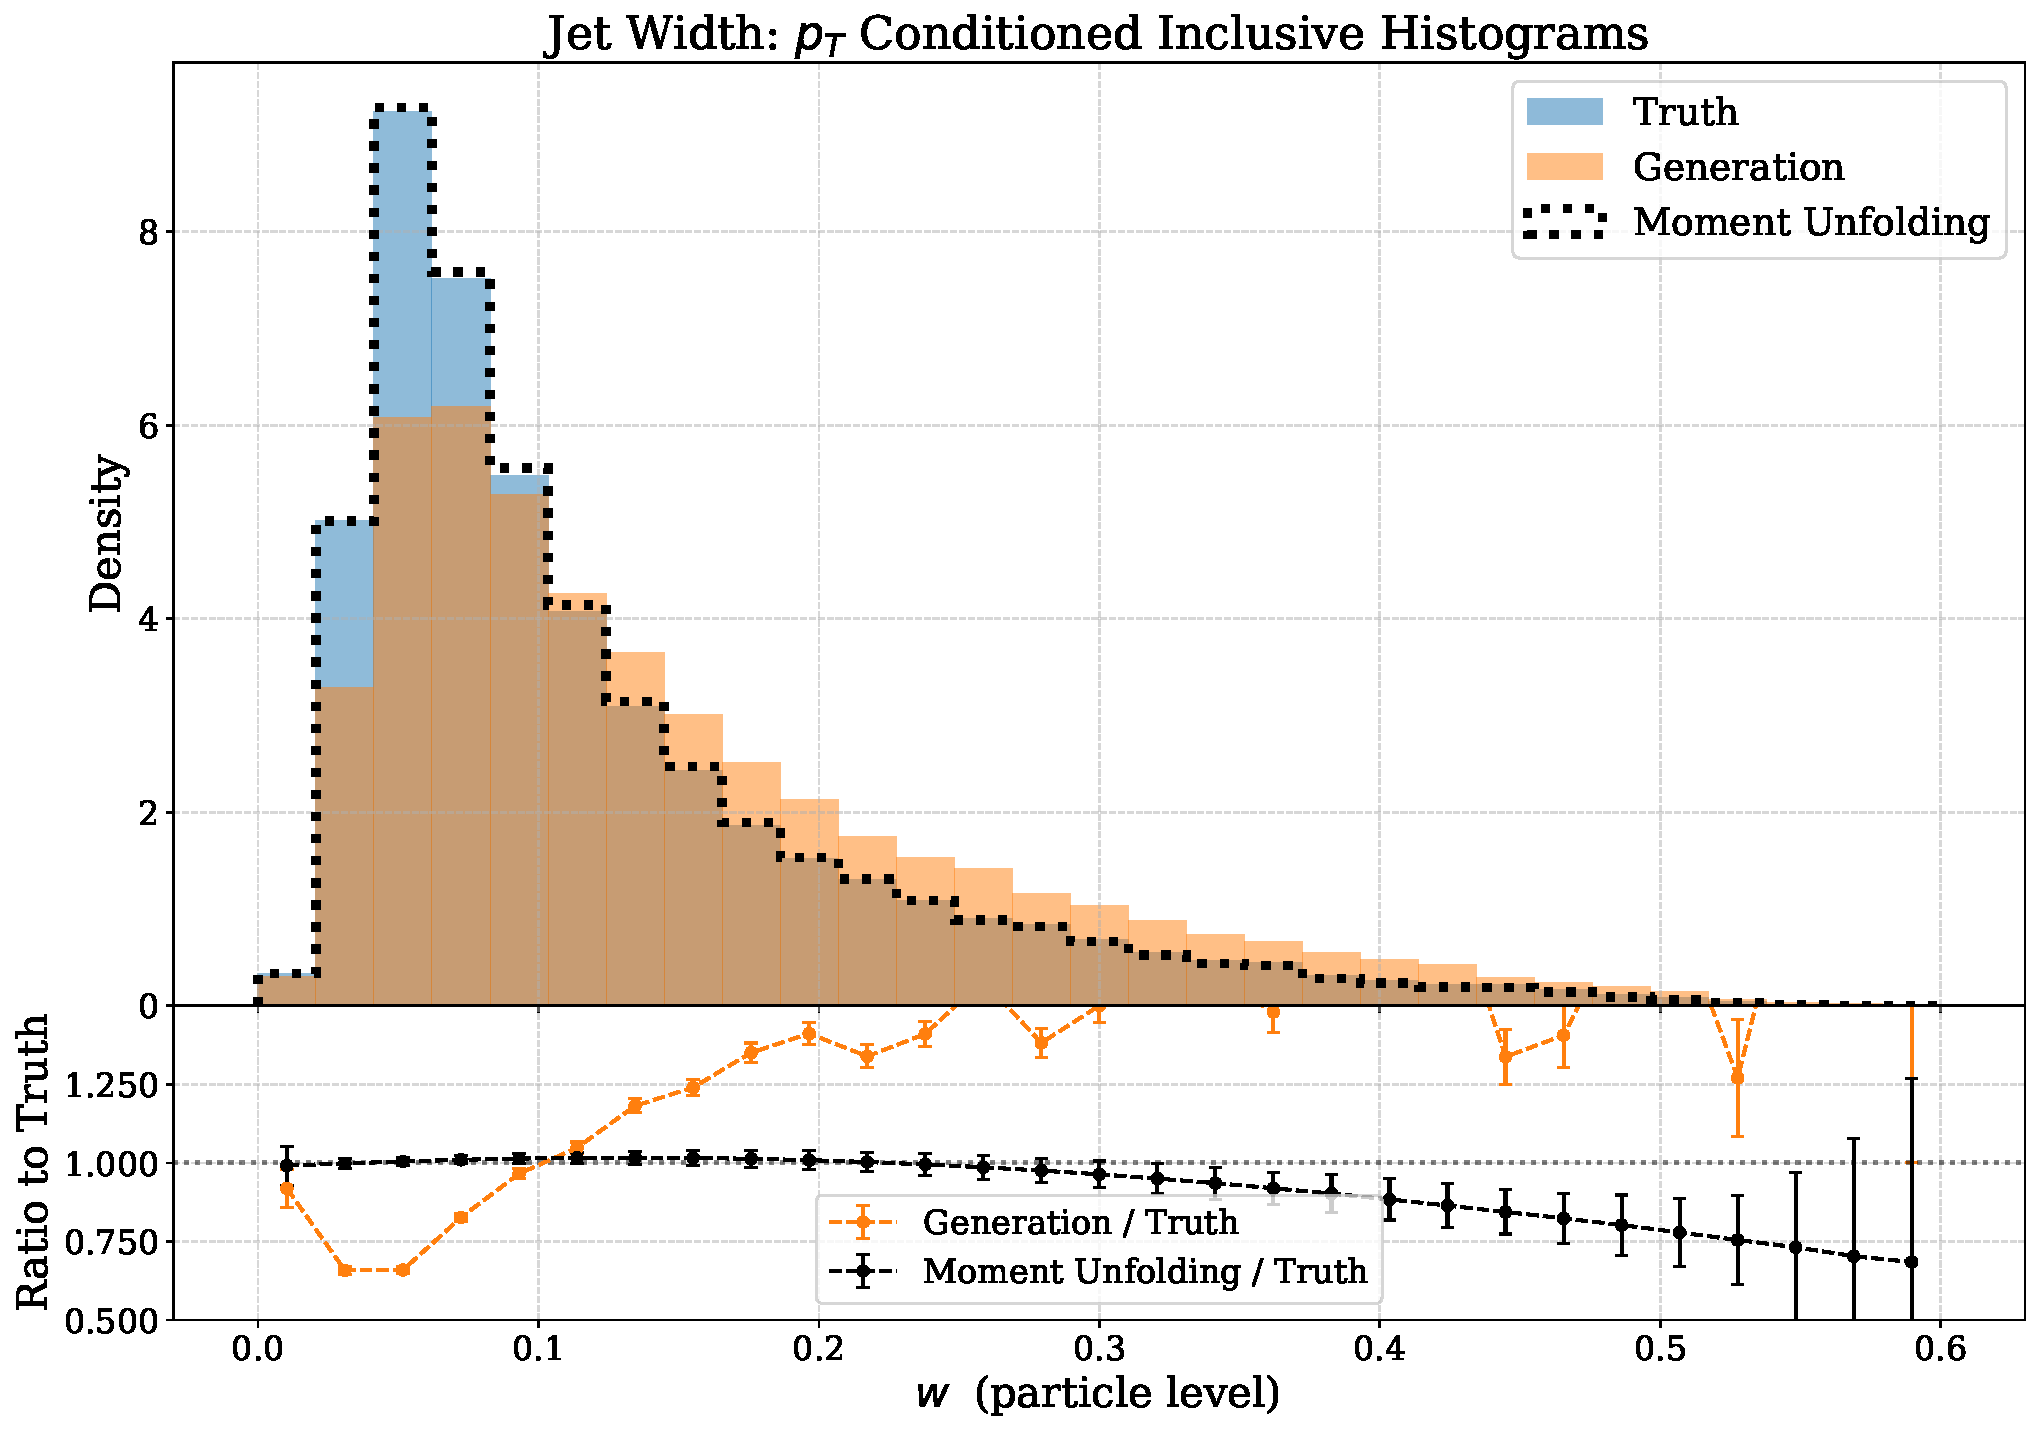
\includegraphics[height=0.32\textwidth]{figures/chapter-05/wpjetexample.pdf}}
    \subfloat[]{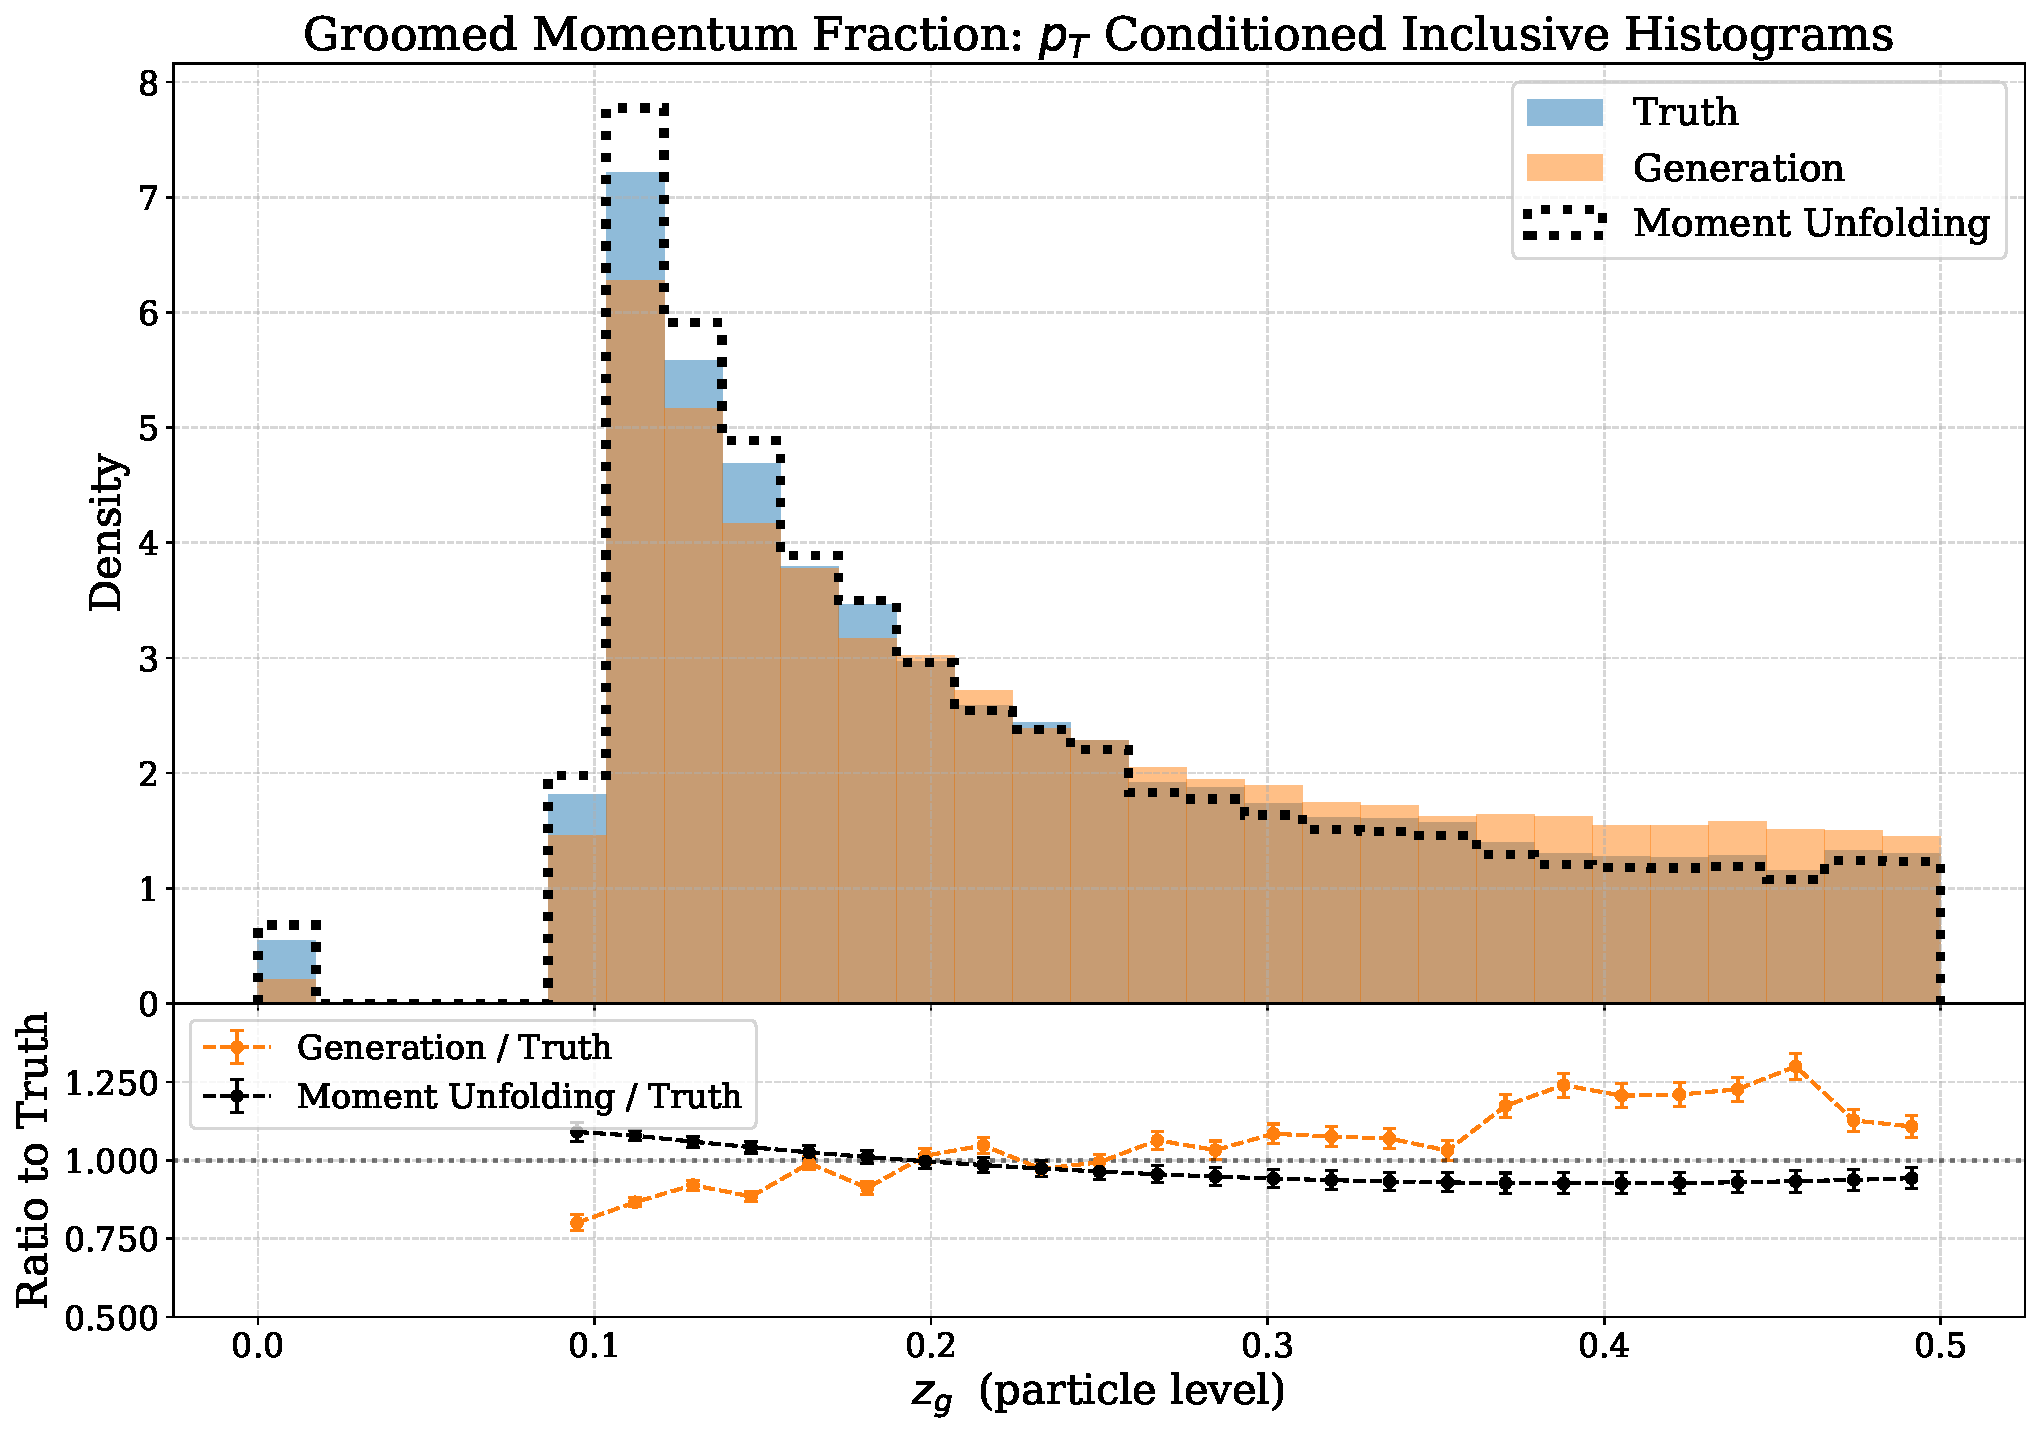
\includegraphics[height=0.32\textwidth]{figures/chapter-05/zgpjetexample.pdf}}
    \caption[Momentum dependent unfolding of inclusive jet substructure distributions]{Inclusive distributions of (a) jet mass, (b) jet charge, (c) jet width, and (d) groomed momentum fraction obtained using momentum dependent \textsc{Moment Unfolding}, where the correction parameters $\beta_a(p_T)$ are functions of jet transverse momentum. The plots compare Truth (\textsc{Herwig}), Generation (\textsc{Pythia}), and reweighted Generation with weights from momentum conditioned \textsc{Moment Unfolding} results. Compared to the momentum independent unfolding shown in Fig.~\ref{fig:jetexample_dists}, the momentum dependent approach achieves notably better agreement with the truth distributions, particularly in regions where jet properties exhibit strong $p_T$ dependence.The lower panel in each plot shows the ratio to truth.}
    \label{fig:pjetexample}
\end{figure}
        \subsubsection{Differential analysis.}
\begin{figure}
    \centering
    \subfloat[]{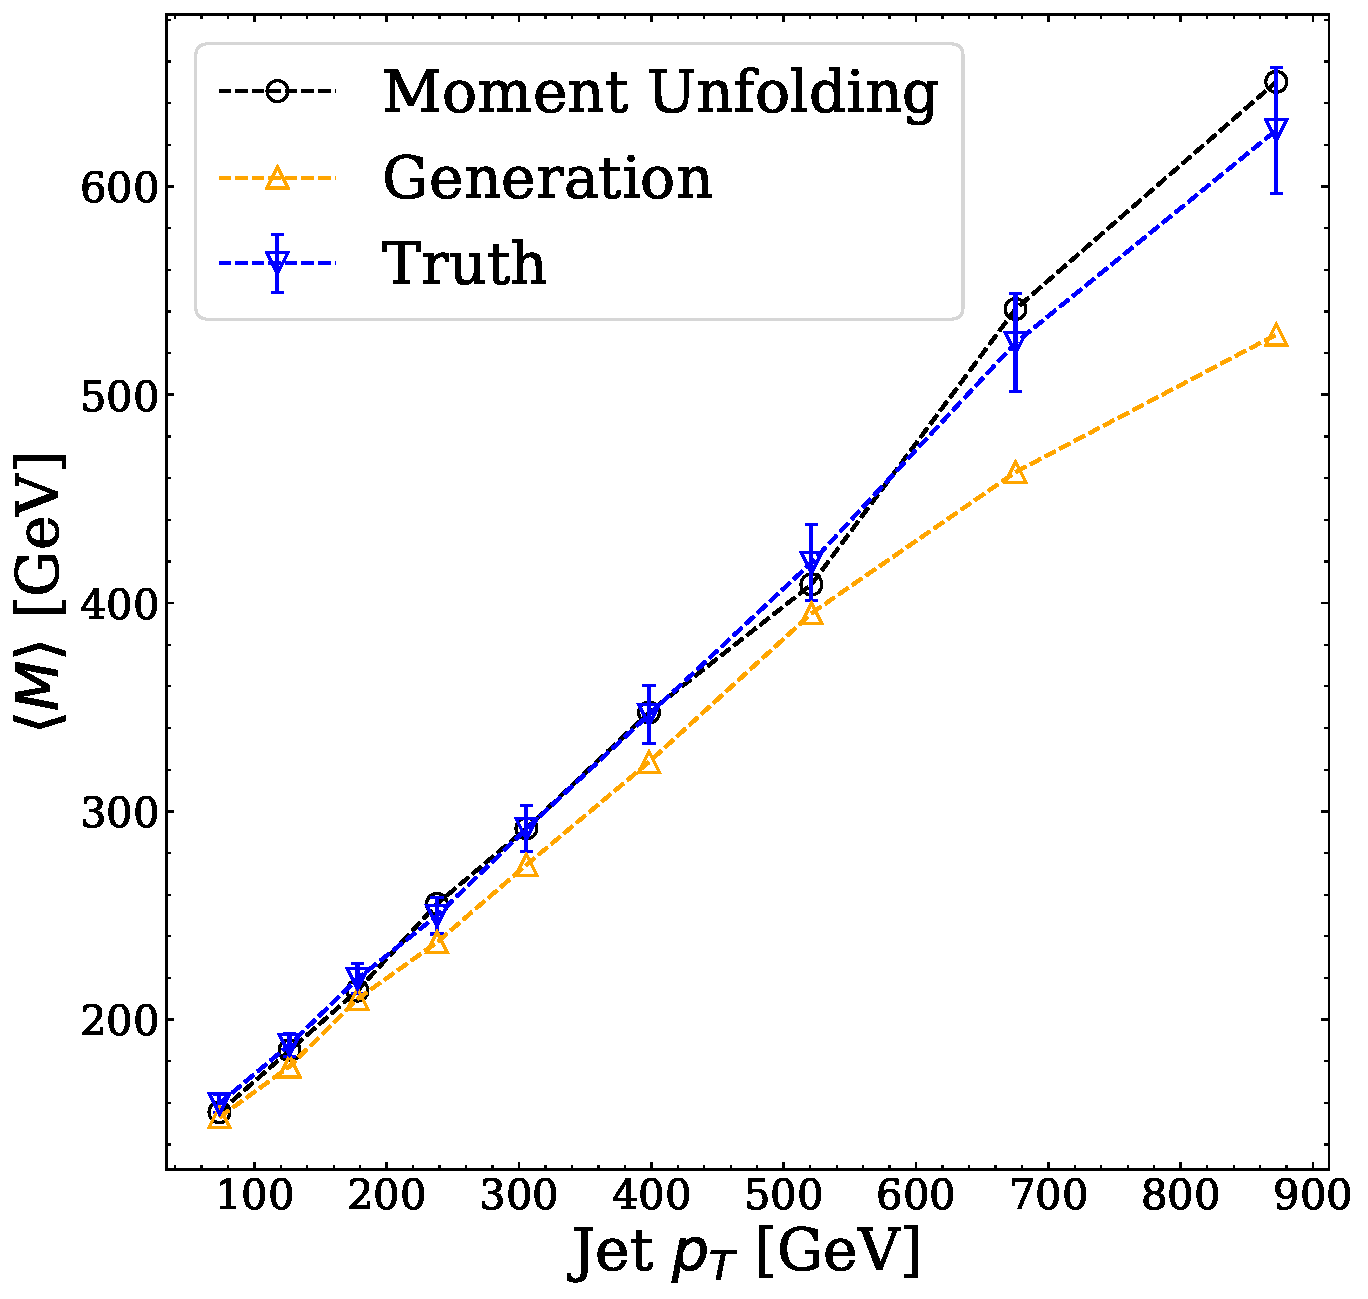
\includegraphics[height=0.4\textwidth]{figures/chapter-05/pmjet1.pdf}
    \label{fig:pmjetmean}}
    \subfloat[]{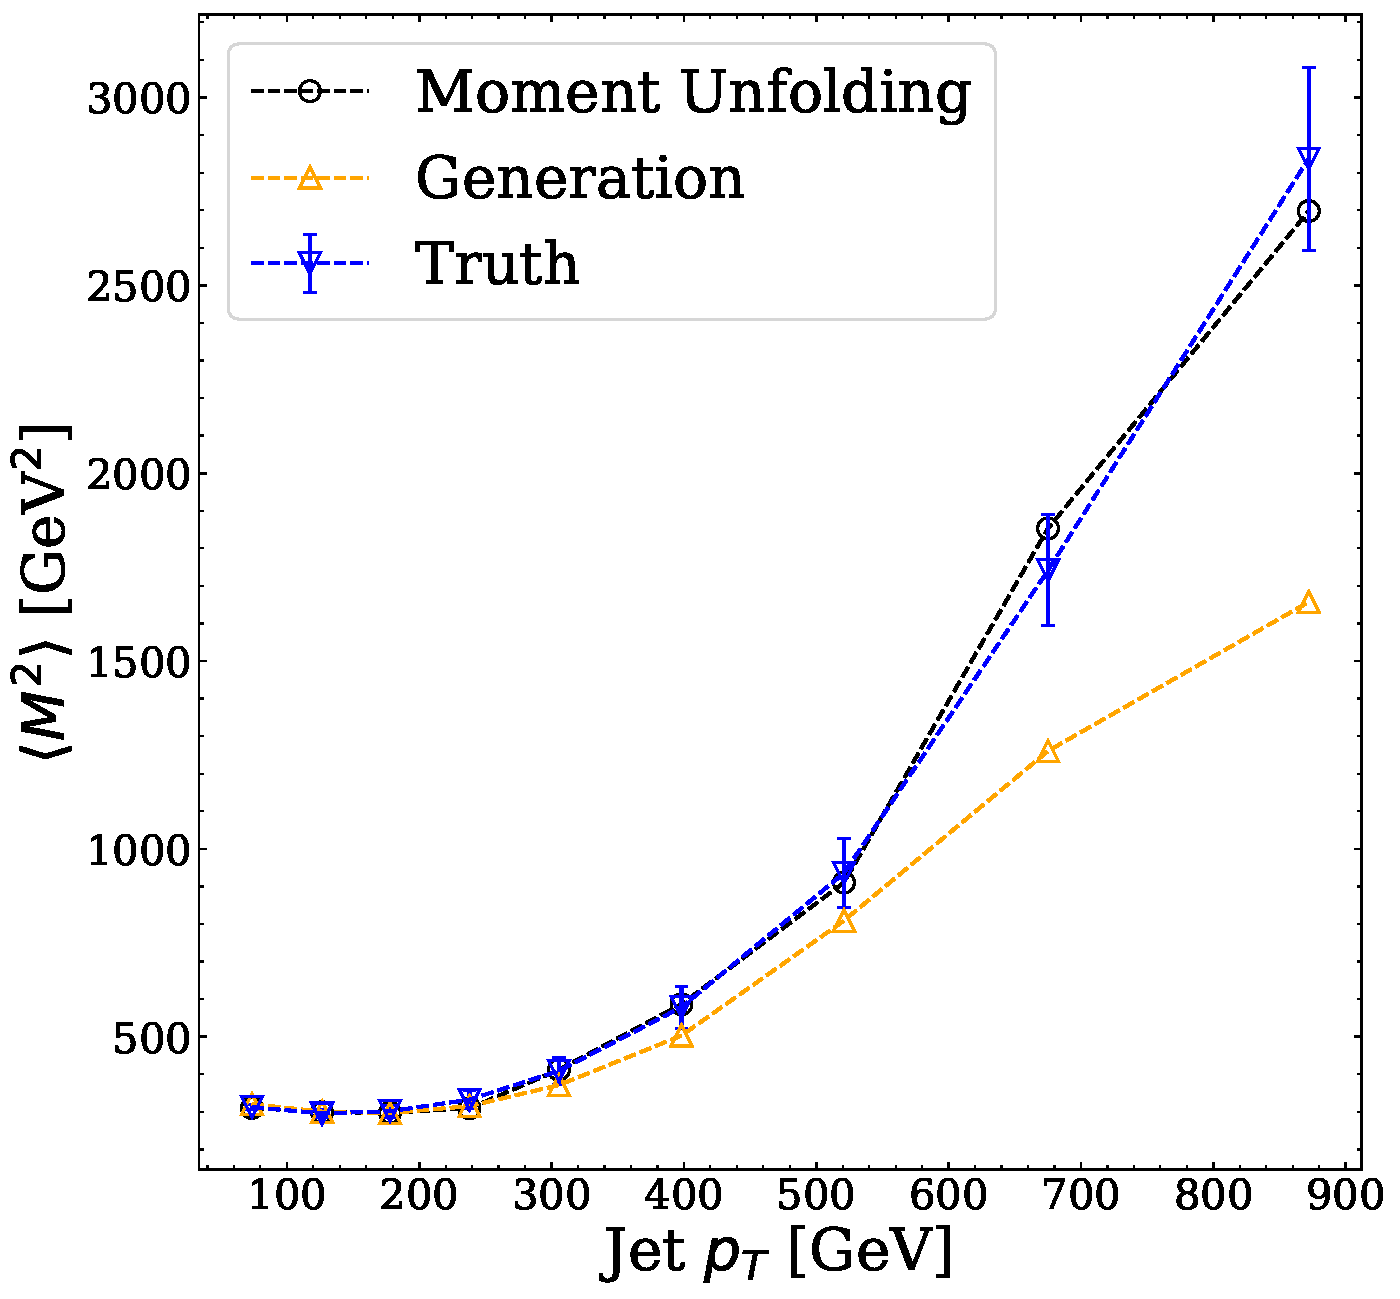
\includegraphics[height=0.4\textwidth]{figures/chapter-05/pmjet2.pdf}
    \label{fig:pmjetvar}}
    \\
    \subfloat[]{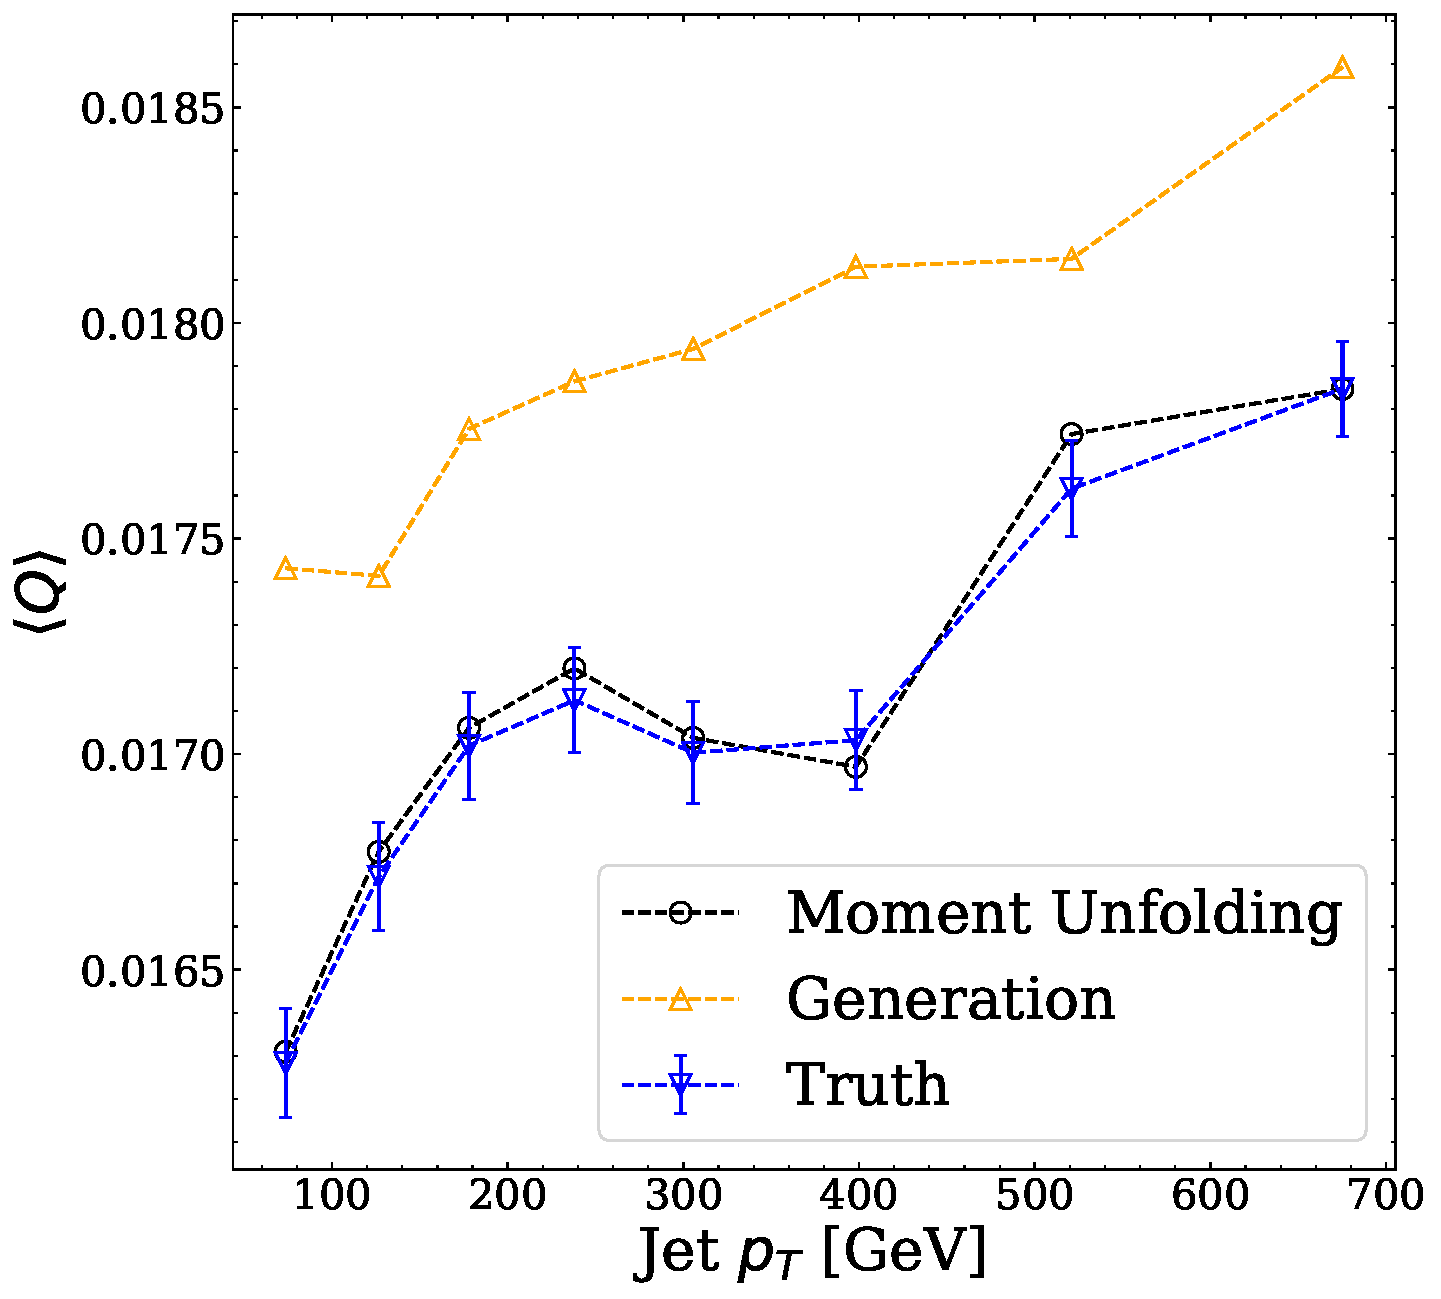
\includegraphics[height=0.4\textwidth]{figures/chapter-05/pqjet1.pdf}
    \label{fig:pqjetmean}}
    \subfloat[]{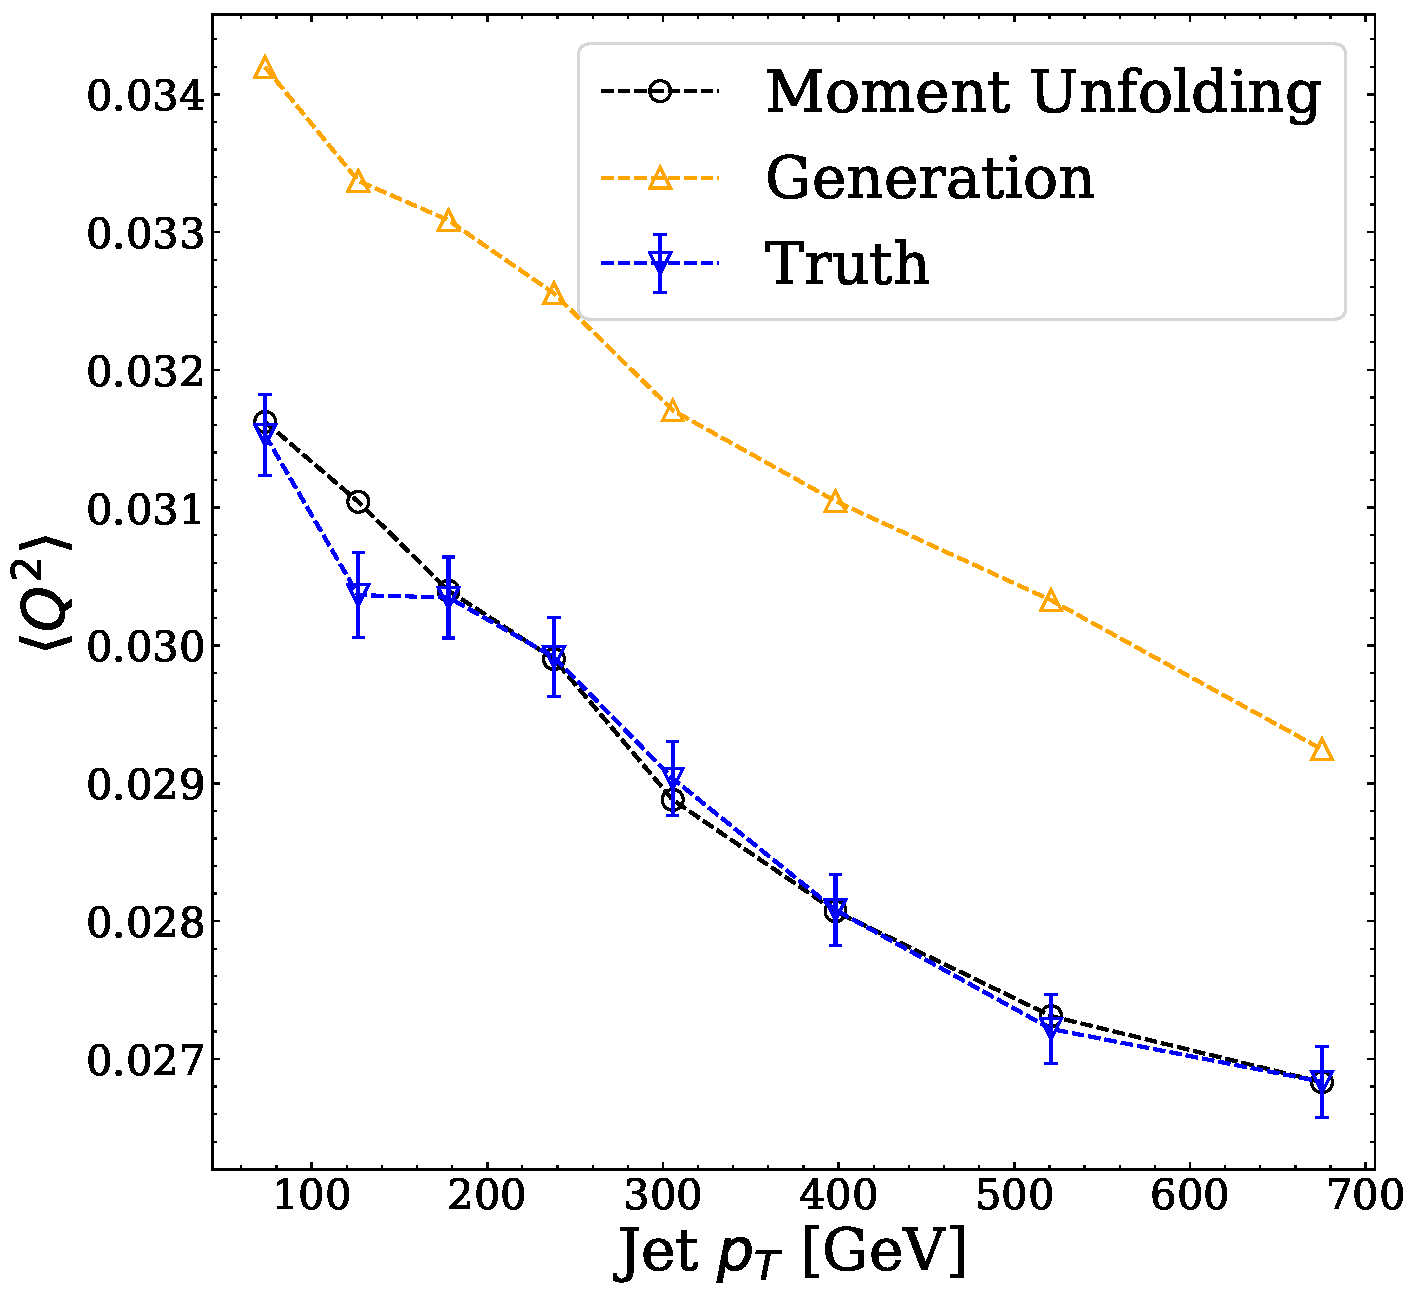
\includegraphics[height=0.4\textwidth]{figures/chapter-05/pqjet2.pdf}
    \label{fig:pqjetvar}}
    \caption[Momentum dependent differential moments of jet substructure observables]{Mean (left column) and variance (right column) of jet substructure observables as a function of jet transverse momentum: (a,b) jet mass, (c,d) jet charge. (Continued on next page.)}
    \label{fig:pjetmoments}
\end{figure}

\begin{figure}
    \ContinuedFloat
    \centering
    \subfloat[]{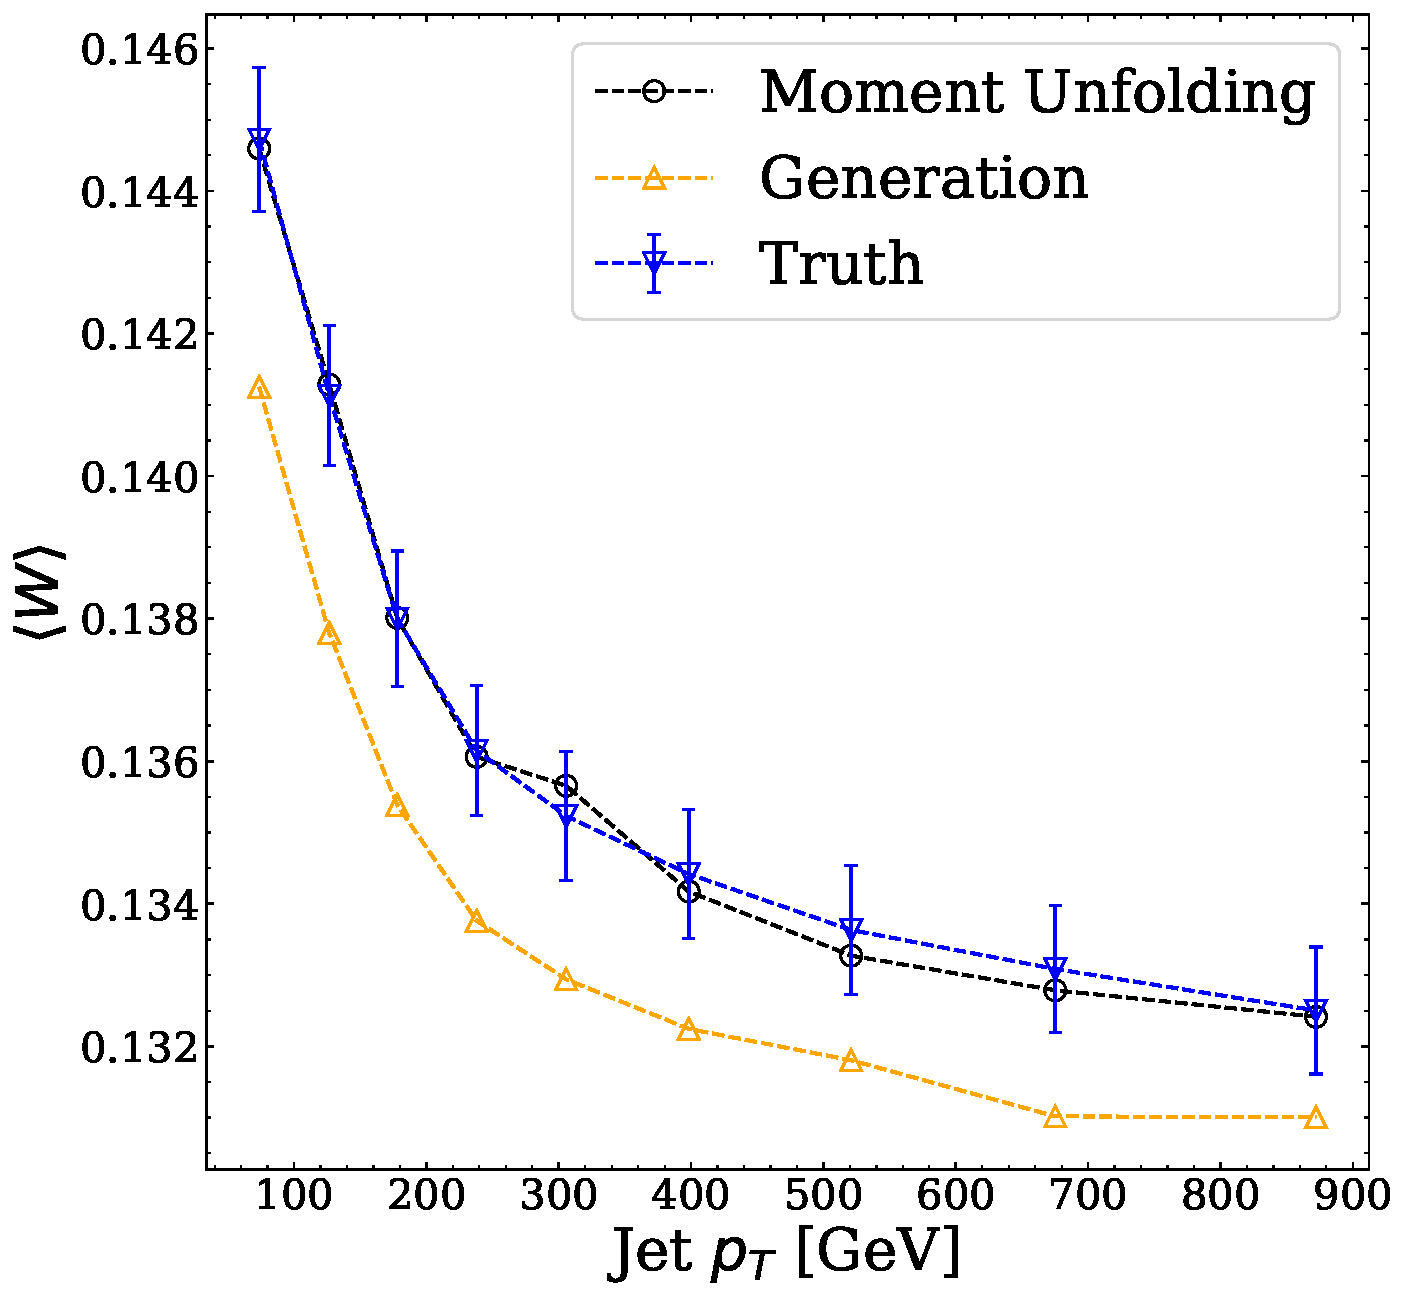
\includegraphics[height=0.4\textwidth]{figures/chapter-05/pwjet1.pdf}
    \label{fig:pwjetmean}}
    \subfloat[]{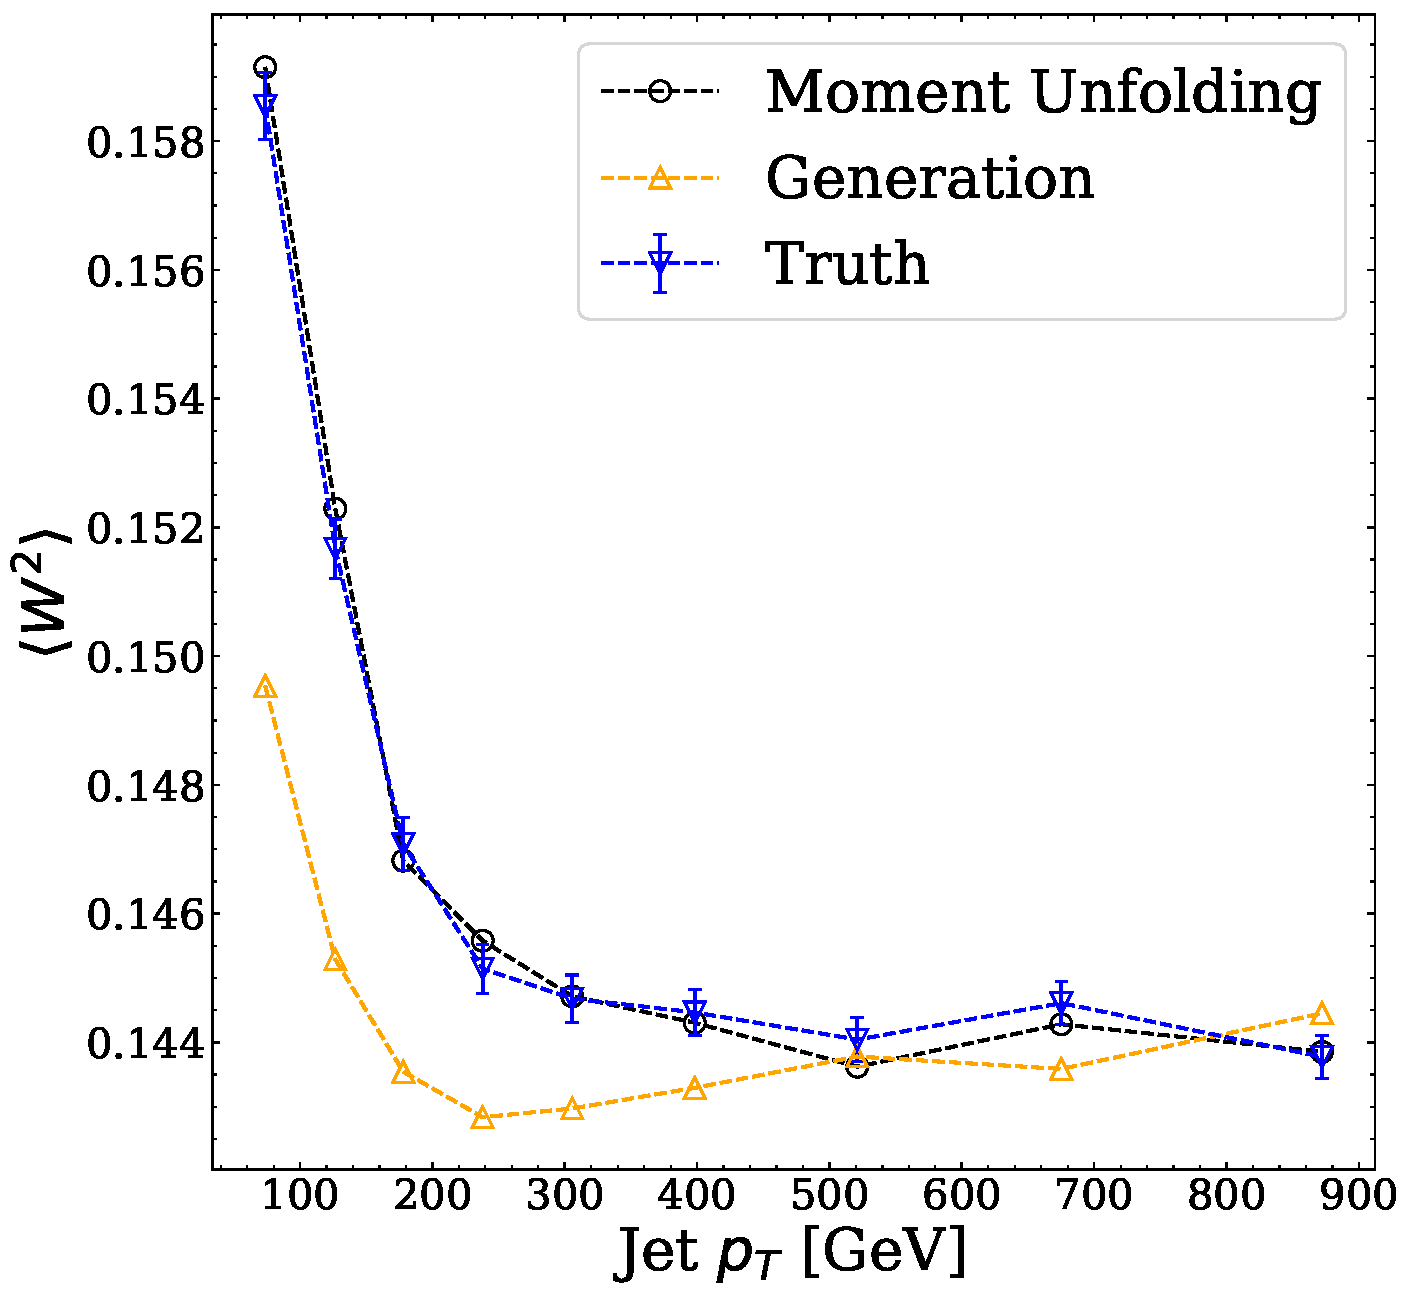
\includegraphics[height=0.4\textwidth]{figures/chapter-05/pwjet2.pdf}
    \label{fig:pwjetvar}}
    \\
    \subfloat[]{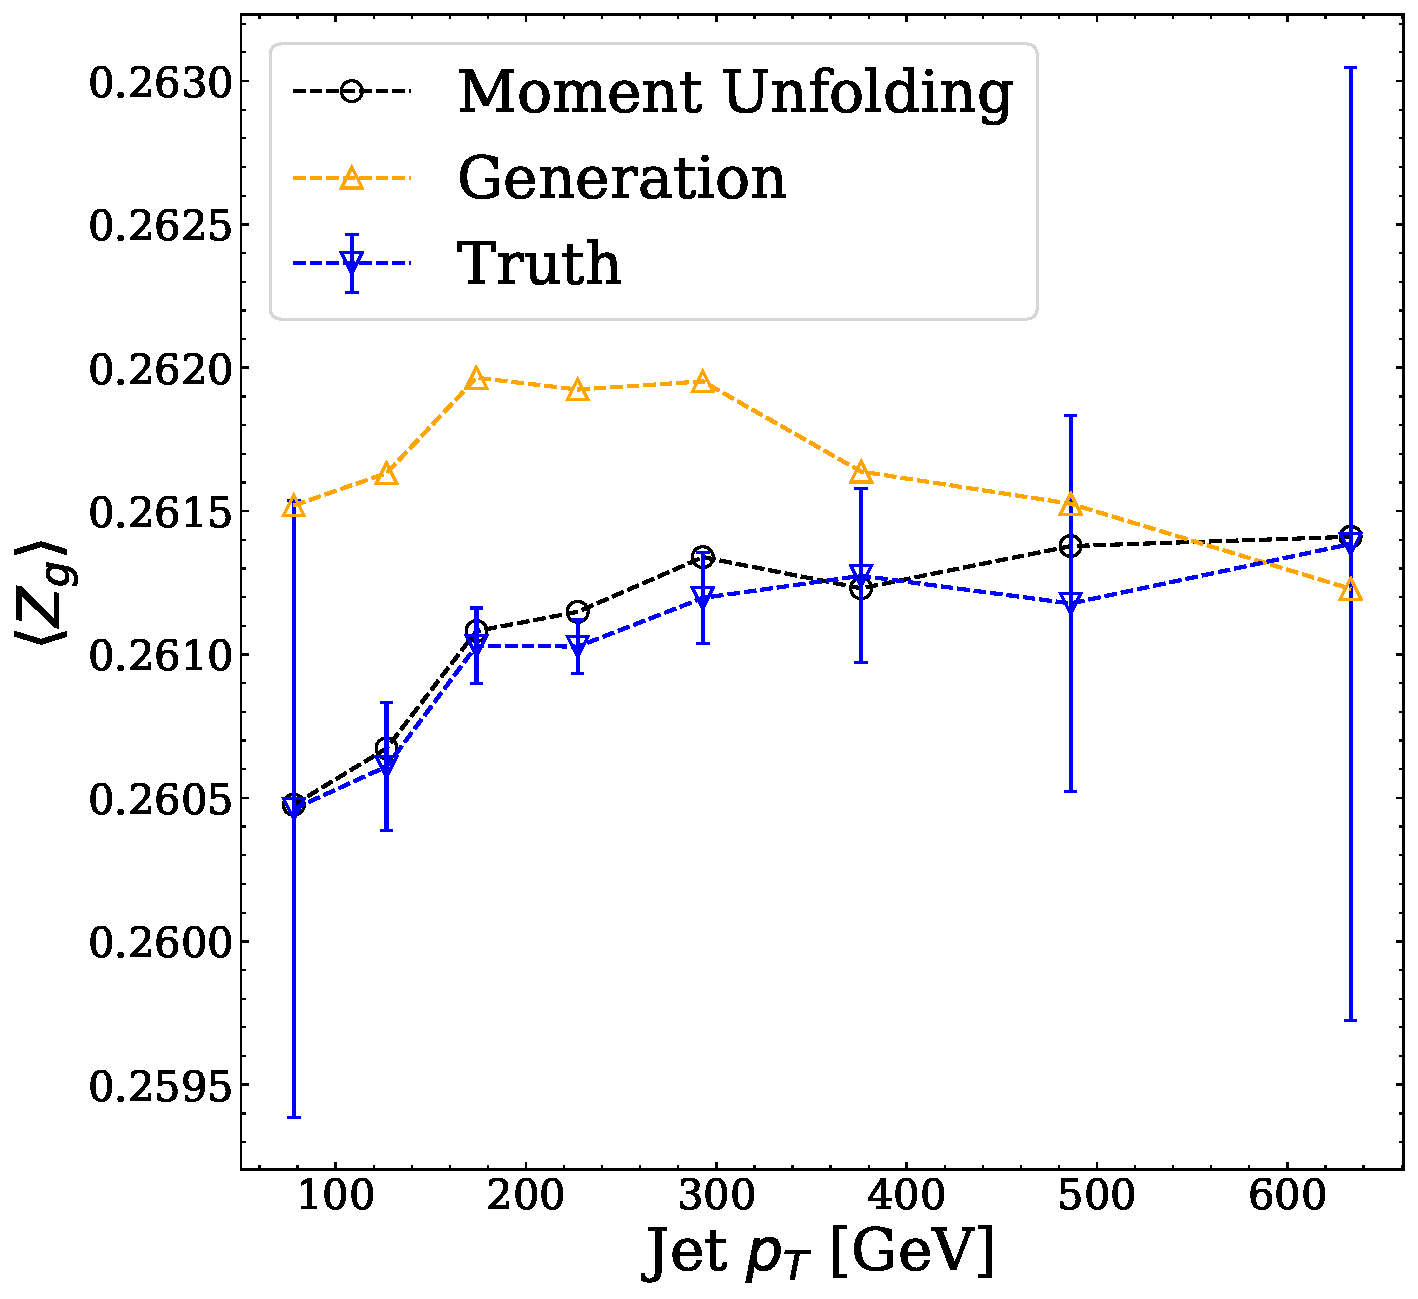
\includegraphics[height=0.4\textwidth]{figures/chapter-05/pzgjet1.pdf}
    \label{fig:pzgjetmean}}
    \subfloat[]{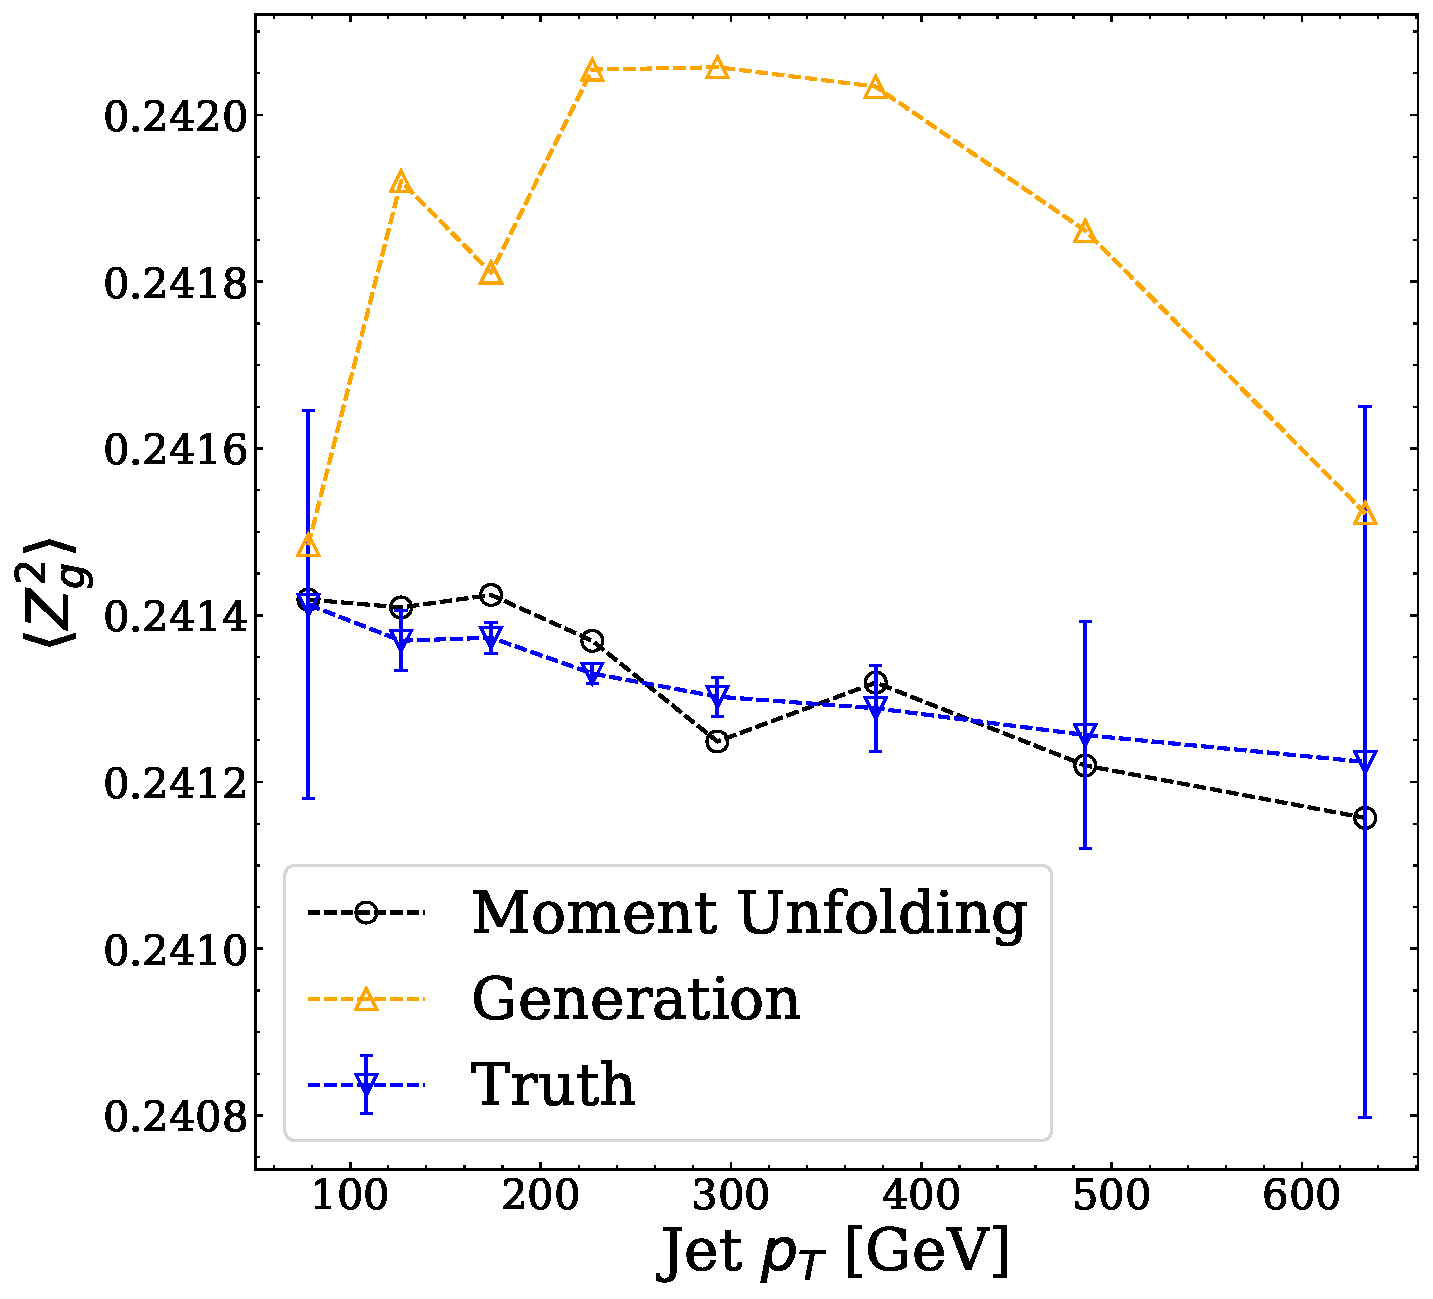
\includegraphics[height=0.4\textwidth]{figures/chapter-05/pzgjet2.pdf}
    \label{fig:pzgjetvar}}
    \caption[]{(Continued from previous page.) Mean (left column) and variance (right column) of jet substructure observables: (e,f) jet width, and (g,h) groomed momentum fraction. The plots compare Truth (\textsc{Herwig}), Generation (\textsc{Pythia}), and reweighted Generation, weighted with momentum dependent \textsc{Moment Unfolding} results. For visual clarity, error bars show only statistical uncertainties on the truth distribution. The \textsc{Moment Unfolding} method successfully reproduces both the mean and variance across the full $p_T$ range, with results consistent with truth within uncertainties.}
\end{figure}

            When the momentum dependent unfolding approach is used for a differential analysis of moments as a function of \(p_T\), it provides a comprehensive understanding of scaling behaviours.
            %
            This dual perspective offers particularly powerful constraints on theoretical models, as it simultaneously tests the overall distribution shapes and their evolution with energy scale.
            %
            \cref{fig:pjetmoments} shows the first and second moments of each observable as a function of $p_T$.

            The results demonstrate that \textsc{Moment Unfolding} successfully recovers the $p_T$ dependent moments of all the observables, capturing the variations in these quantities with jet \(p_T\).
            %
            This capability is particularly valuable for testing theoretical predictions of how jet properties scale with energy, a fundamental aspect of QCD phenomenology.

            These momentum dependent results allow us to analyse the scaling behaviour of each observable.
            %
            The jet mass shows expected direct scaling with $p_T$, consistent with theoretical expectations from perturbative QCD~\cite{ManganoINTRODUCTIONQCD, ParticleDataGroup:2020ssz, Czakon:2021mjy, CMS:2019fak, ALICE:2020pga, kogler_jet_2019, ALICE:2021njq, Dasgupta:2022fim, ATLAS:2014bjq},
            %
            the mean jet charge decreases slightly with increasing $p_T$, reflecting the increased role of gluon radiation at higher energies~\cite{ATLAS:2015rlw, CMS:2017yer, Li:2019dre},
            %
            the jet width decreases with $p_T$, consistent with the collimation of high--energy jets due to the Lorentz boost~\cite{ATLAS:2014hvo, ATLAS:2011lgt}, and
            %
            the groomed momentum fraction shows minimal $p_T$ dependence, a feature expected from the scale--invariant nature of the splitting functions in QCD~\cite{ATLAS:2020bbn, CMS:2020poo, ATLASCollaboration2025ElectroweakLHC}.

            These results not only validate the \textsc{Moment Unfolding} method but also demonstrate its utility for extracting physically meaningful insights about jet formation and evolution.
            %
            These scaling behaviours, when applied to real collider data, could serve as stringent tests of perturbative QCD and provide constraints on Monte Carlo tuning parameters.
            
\section{Comparison with alternative methods.}
    To assess the performance of \textsc{Moment Unfolding} relative to existing approaches, this section compares the results from \textsc{Moment Unfolding} with those obtained from two alternative methods,
    \begin{enumerate}
        \item \textbf{\textsc{OmniFold}}: A state of the art unbinned unfolding method that reconstructs the full distribution, from which moments can be computed, and 
        \item \textbf{Iterative Bayesian unfolding (IBU)}: A traditional binned unfolding method followed by moment calculation.
    \end{enumerate}
\begin{figure}
    \centering
    \subfloat[]{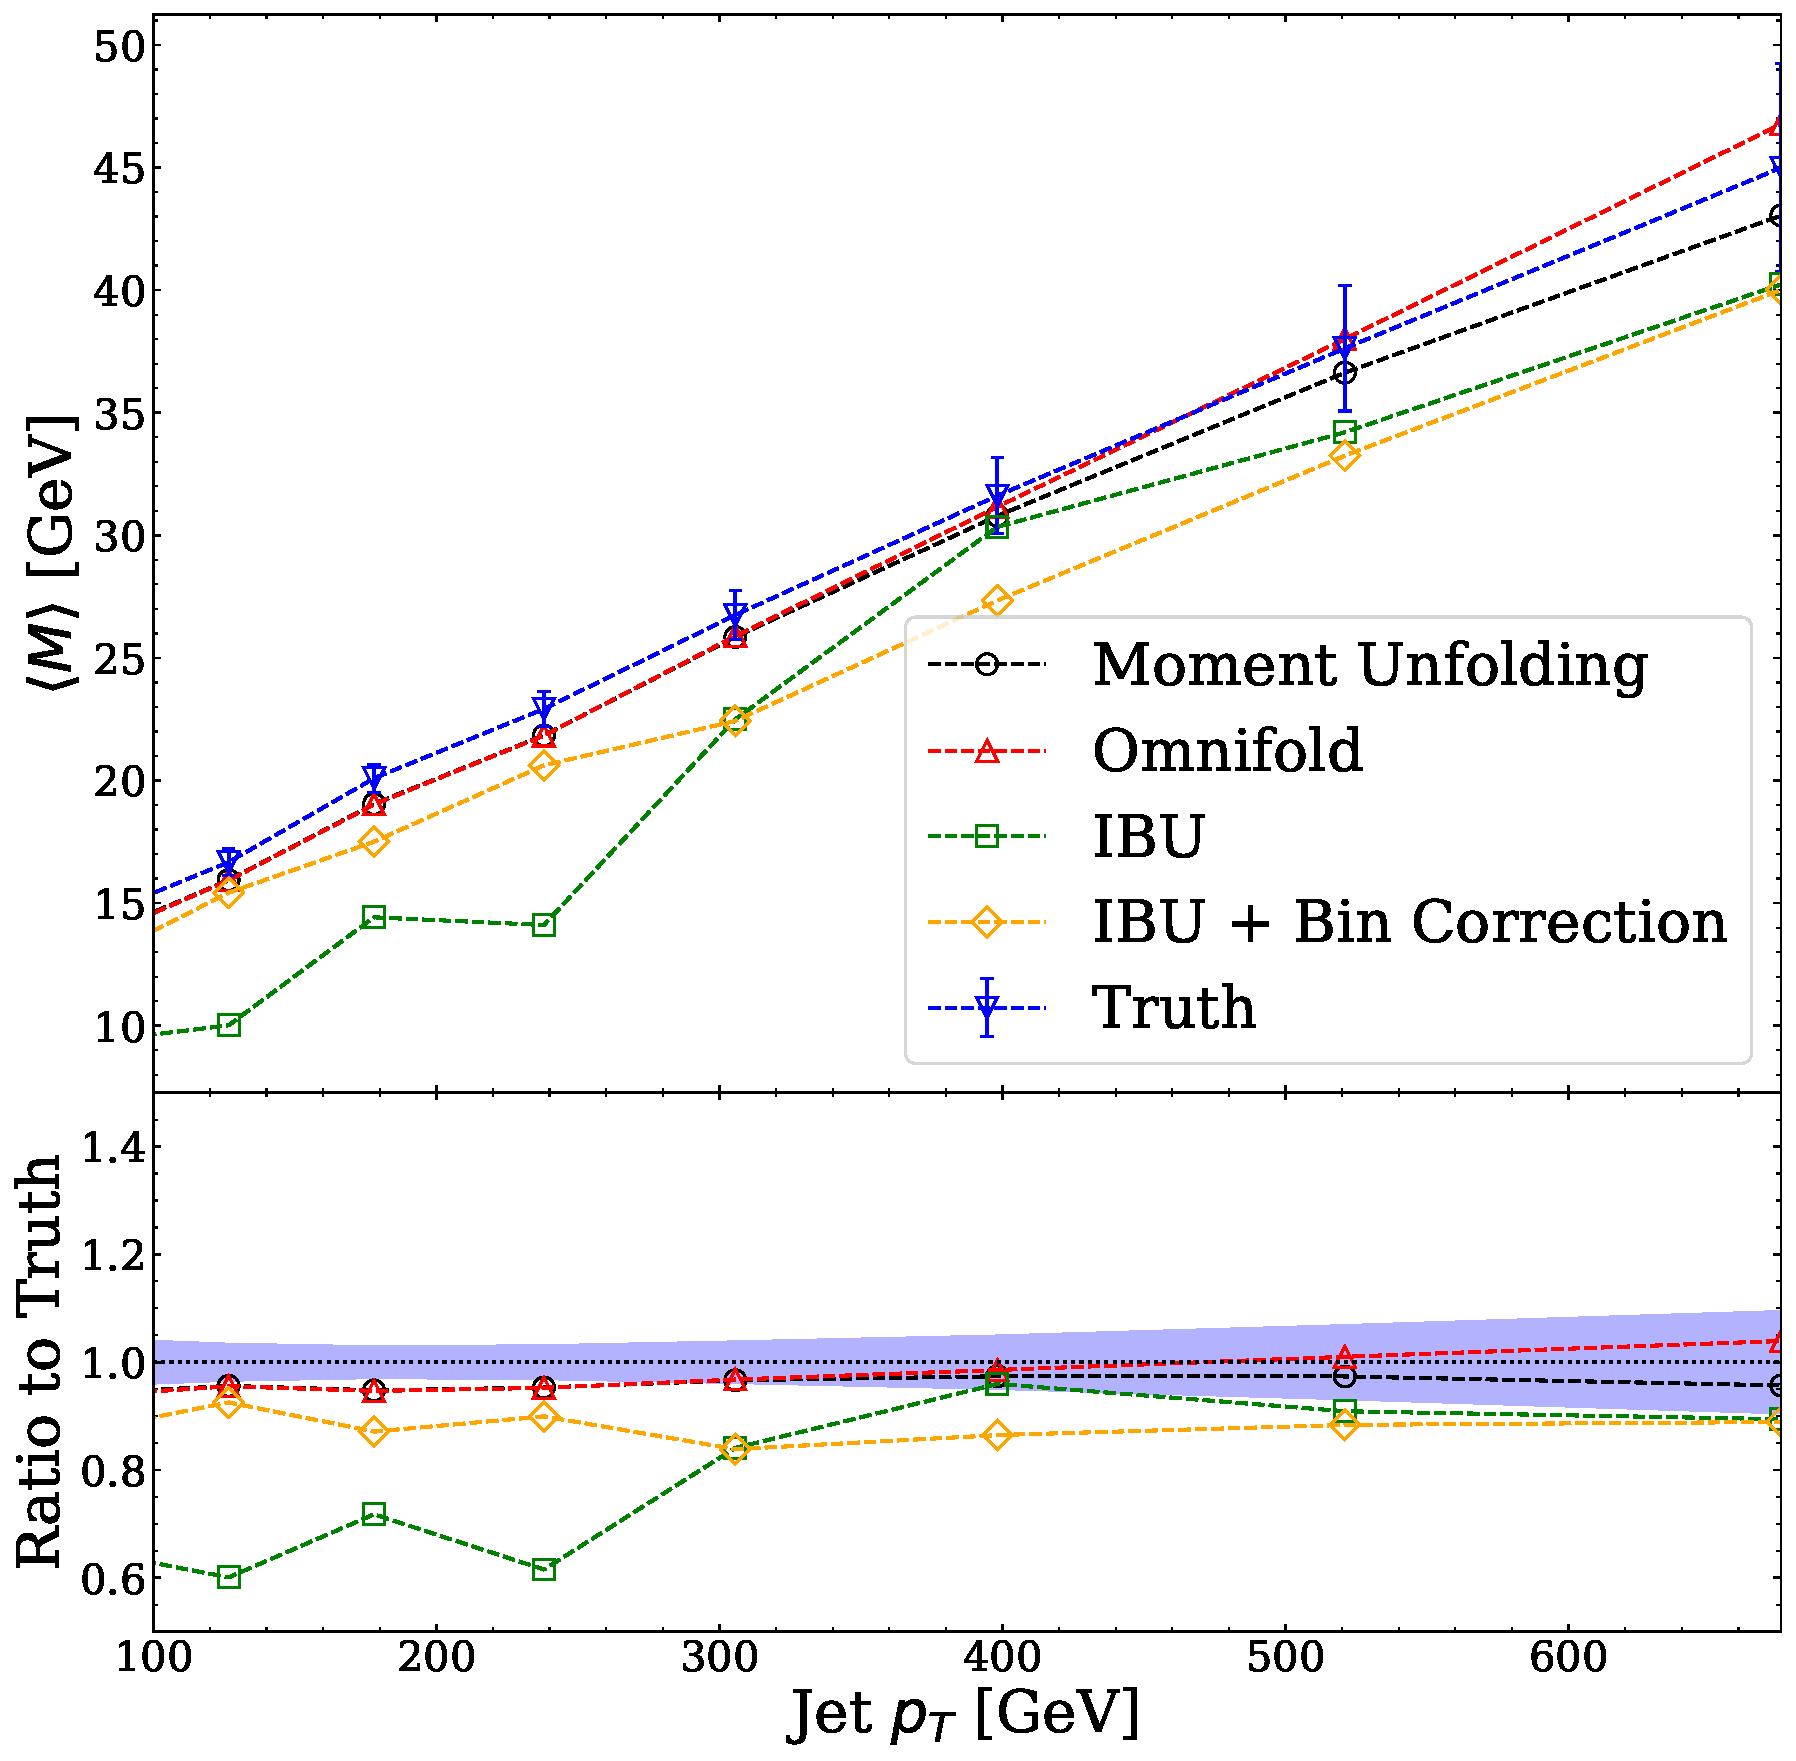
\includegraphics[height=0.45\textwidth]{figures/chapter-05/moment1_m_v_pT.pdf}}
    \subfloat[]{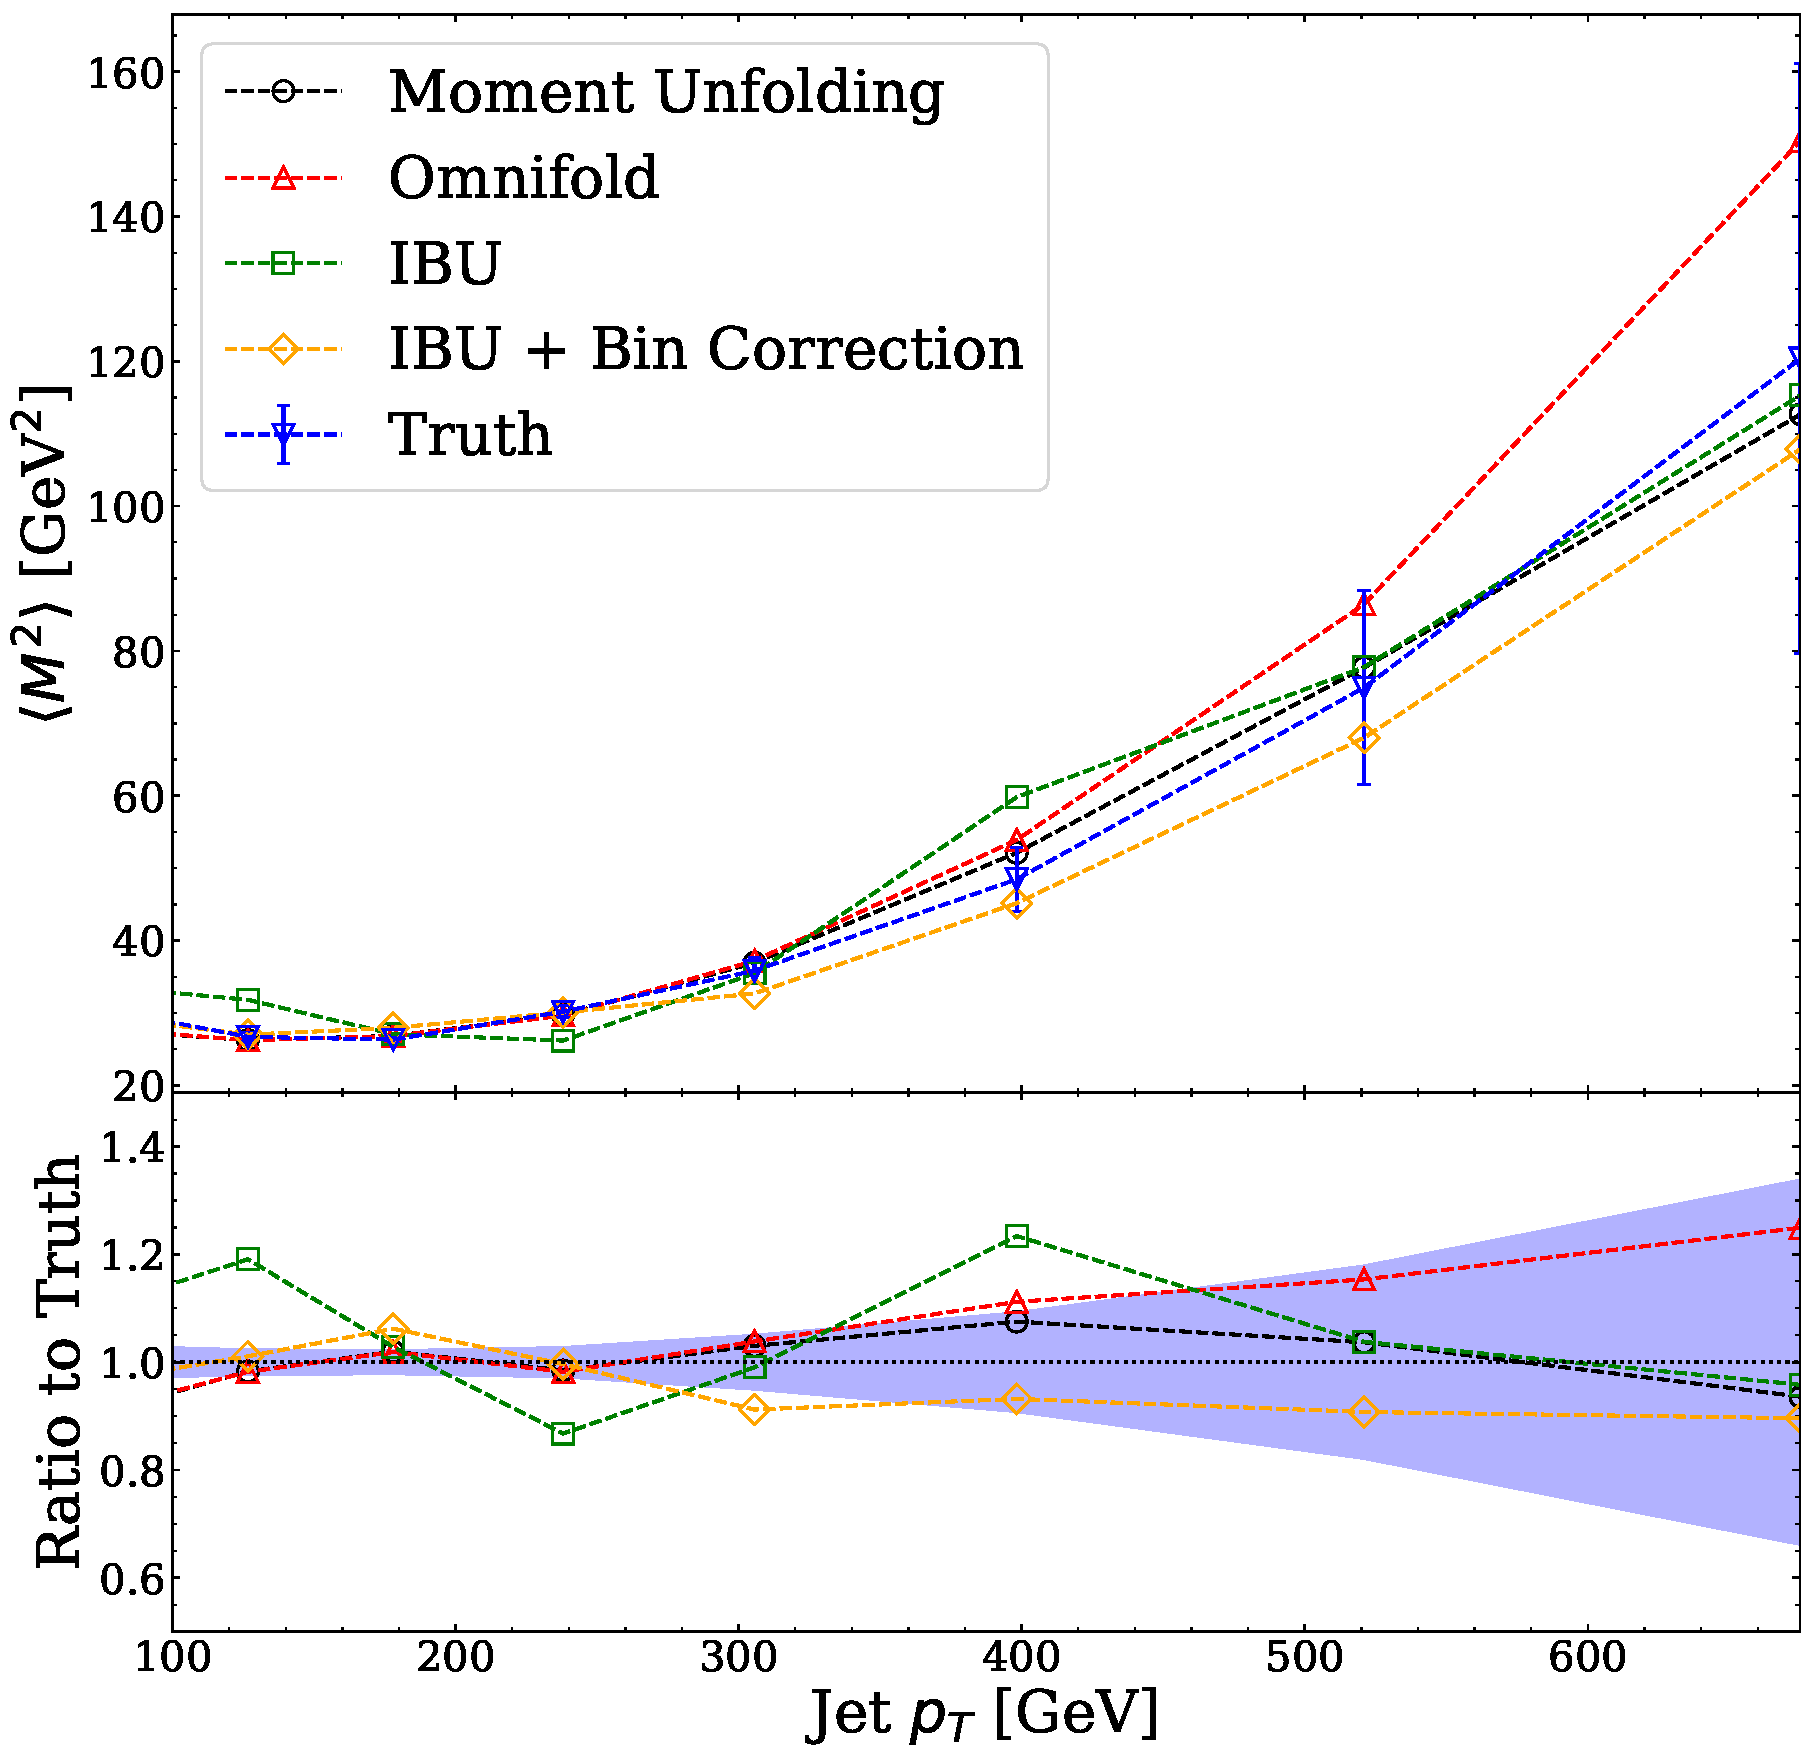
\includegraphics[height=0.45\textwidth]{figures/chapter-05/moment2_m_v_pT.pdf}}\\

    \subfloat[]{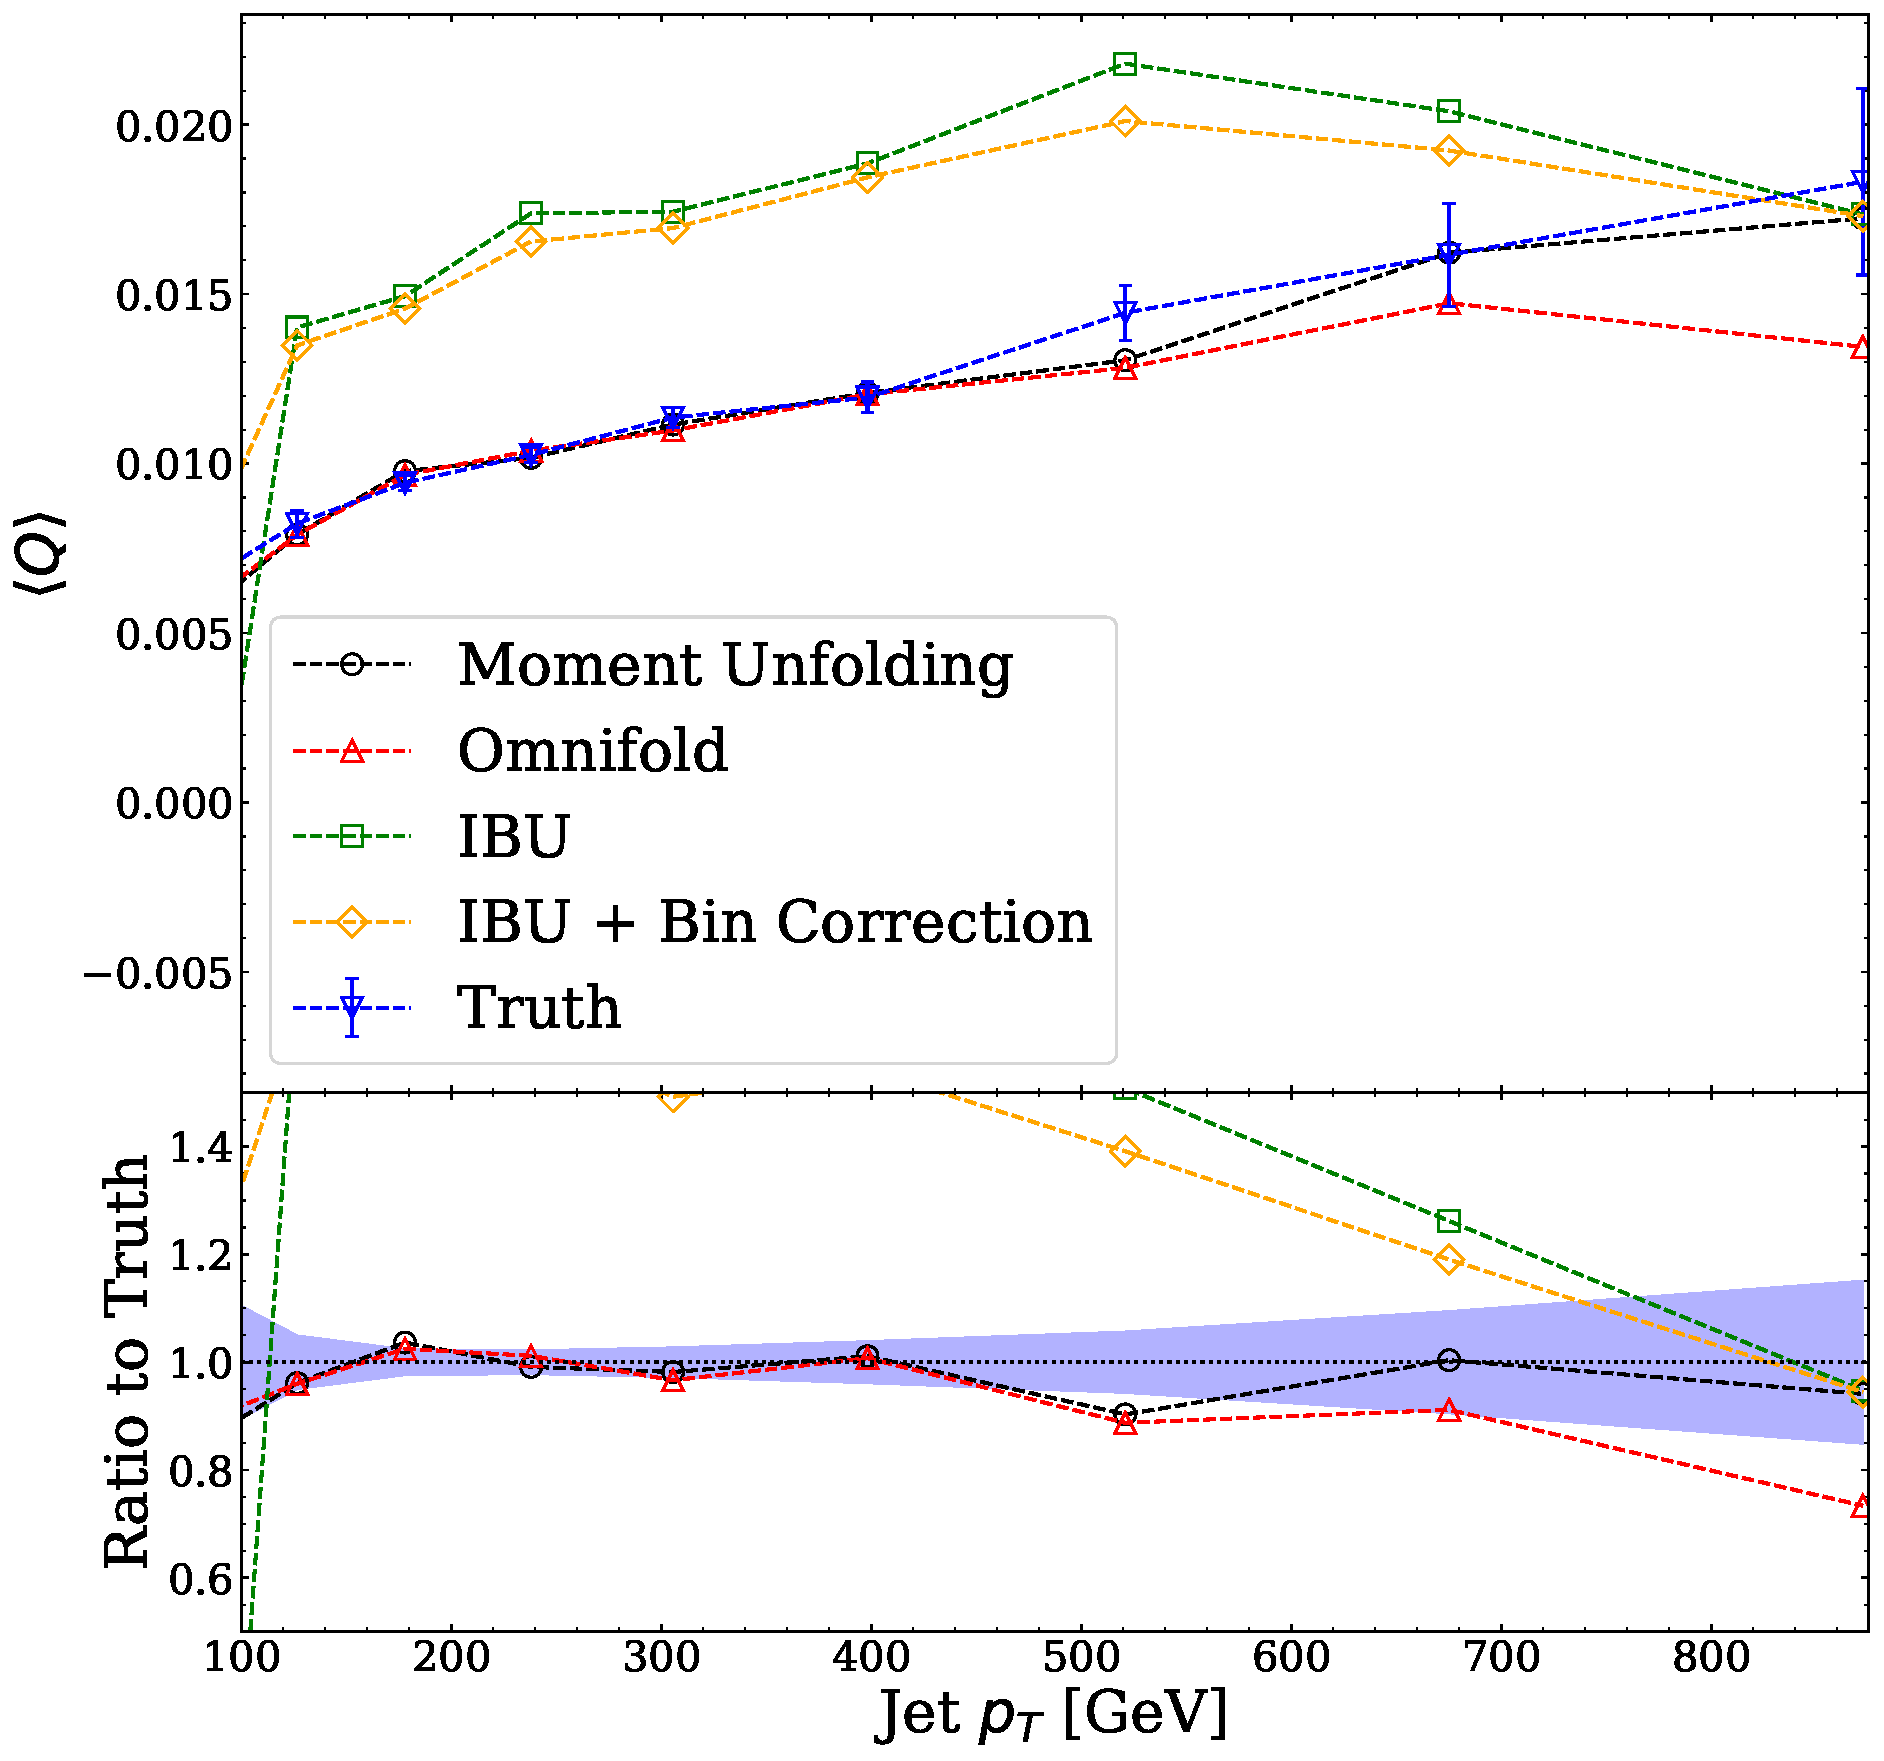
\includegraphics[height=0.45\textwidth]{figures/chapter-05/moment1_q_v_pT.pdf}}
    \subfloat[]{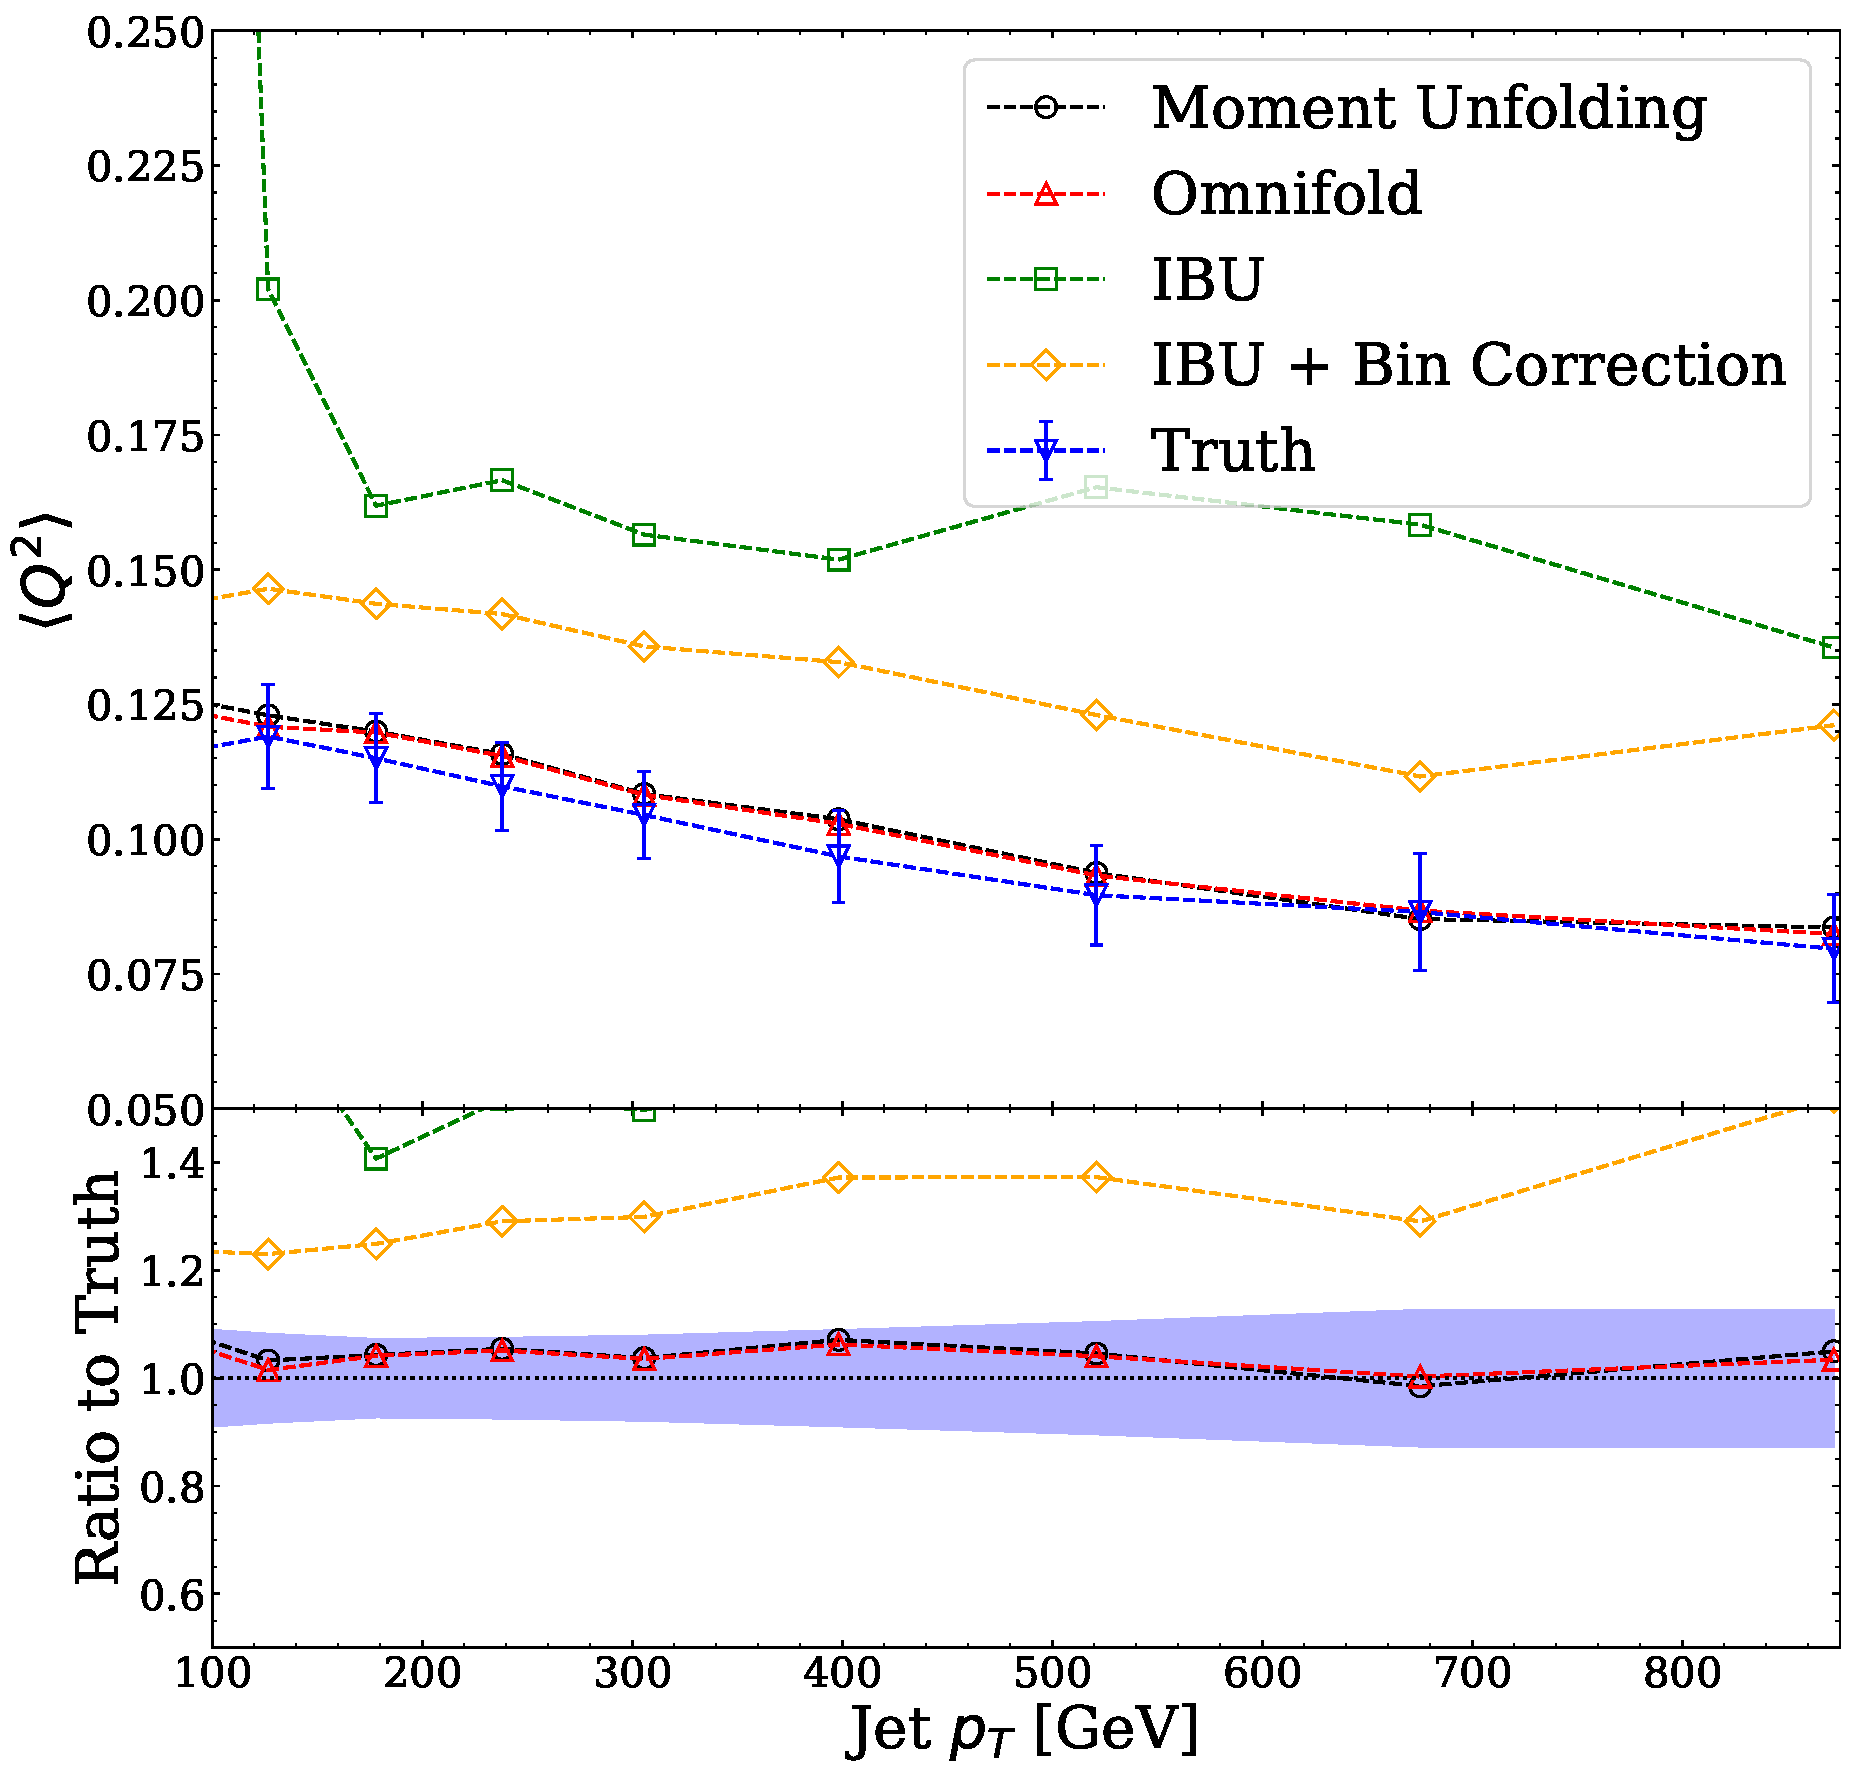
\includegraphics[height=0.45\textwidth]{figures/chapter-05/moment2_q_v_pT.pdf}}
    
    \caption[Comparison of unfolding methods for momentum-dependent jet moments]{Comparison of different unfolding methods for extracting momentum dependent moments of jet substructure observables. Mean (left column) and variance (right column) are shown for (a,b) jet mass and (c,d) jet charge as a function of jet transverse momentum. (Continued on next page.)}
    \label{fig:method-comparison}
\end{figure}

\begin{figure}
    \ContinuedFloat
    \centering
    \subfloat[]{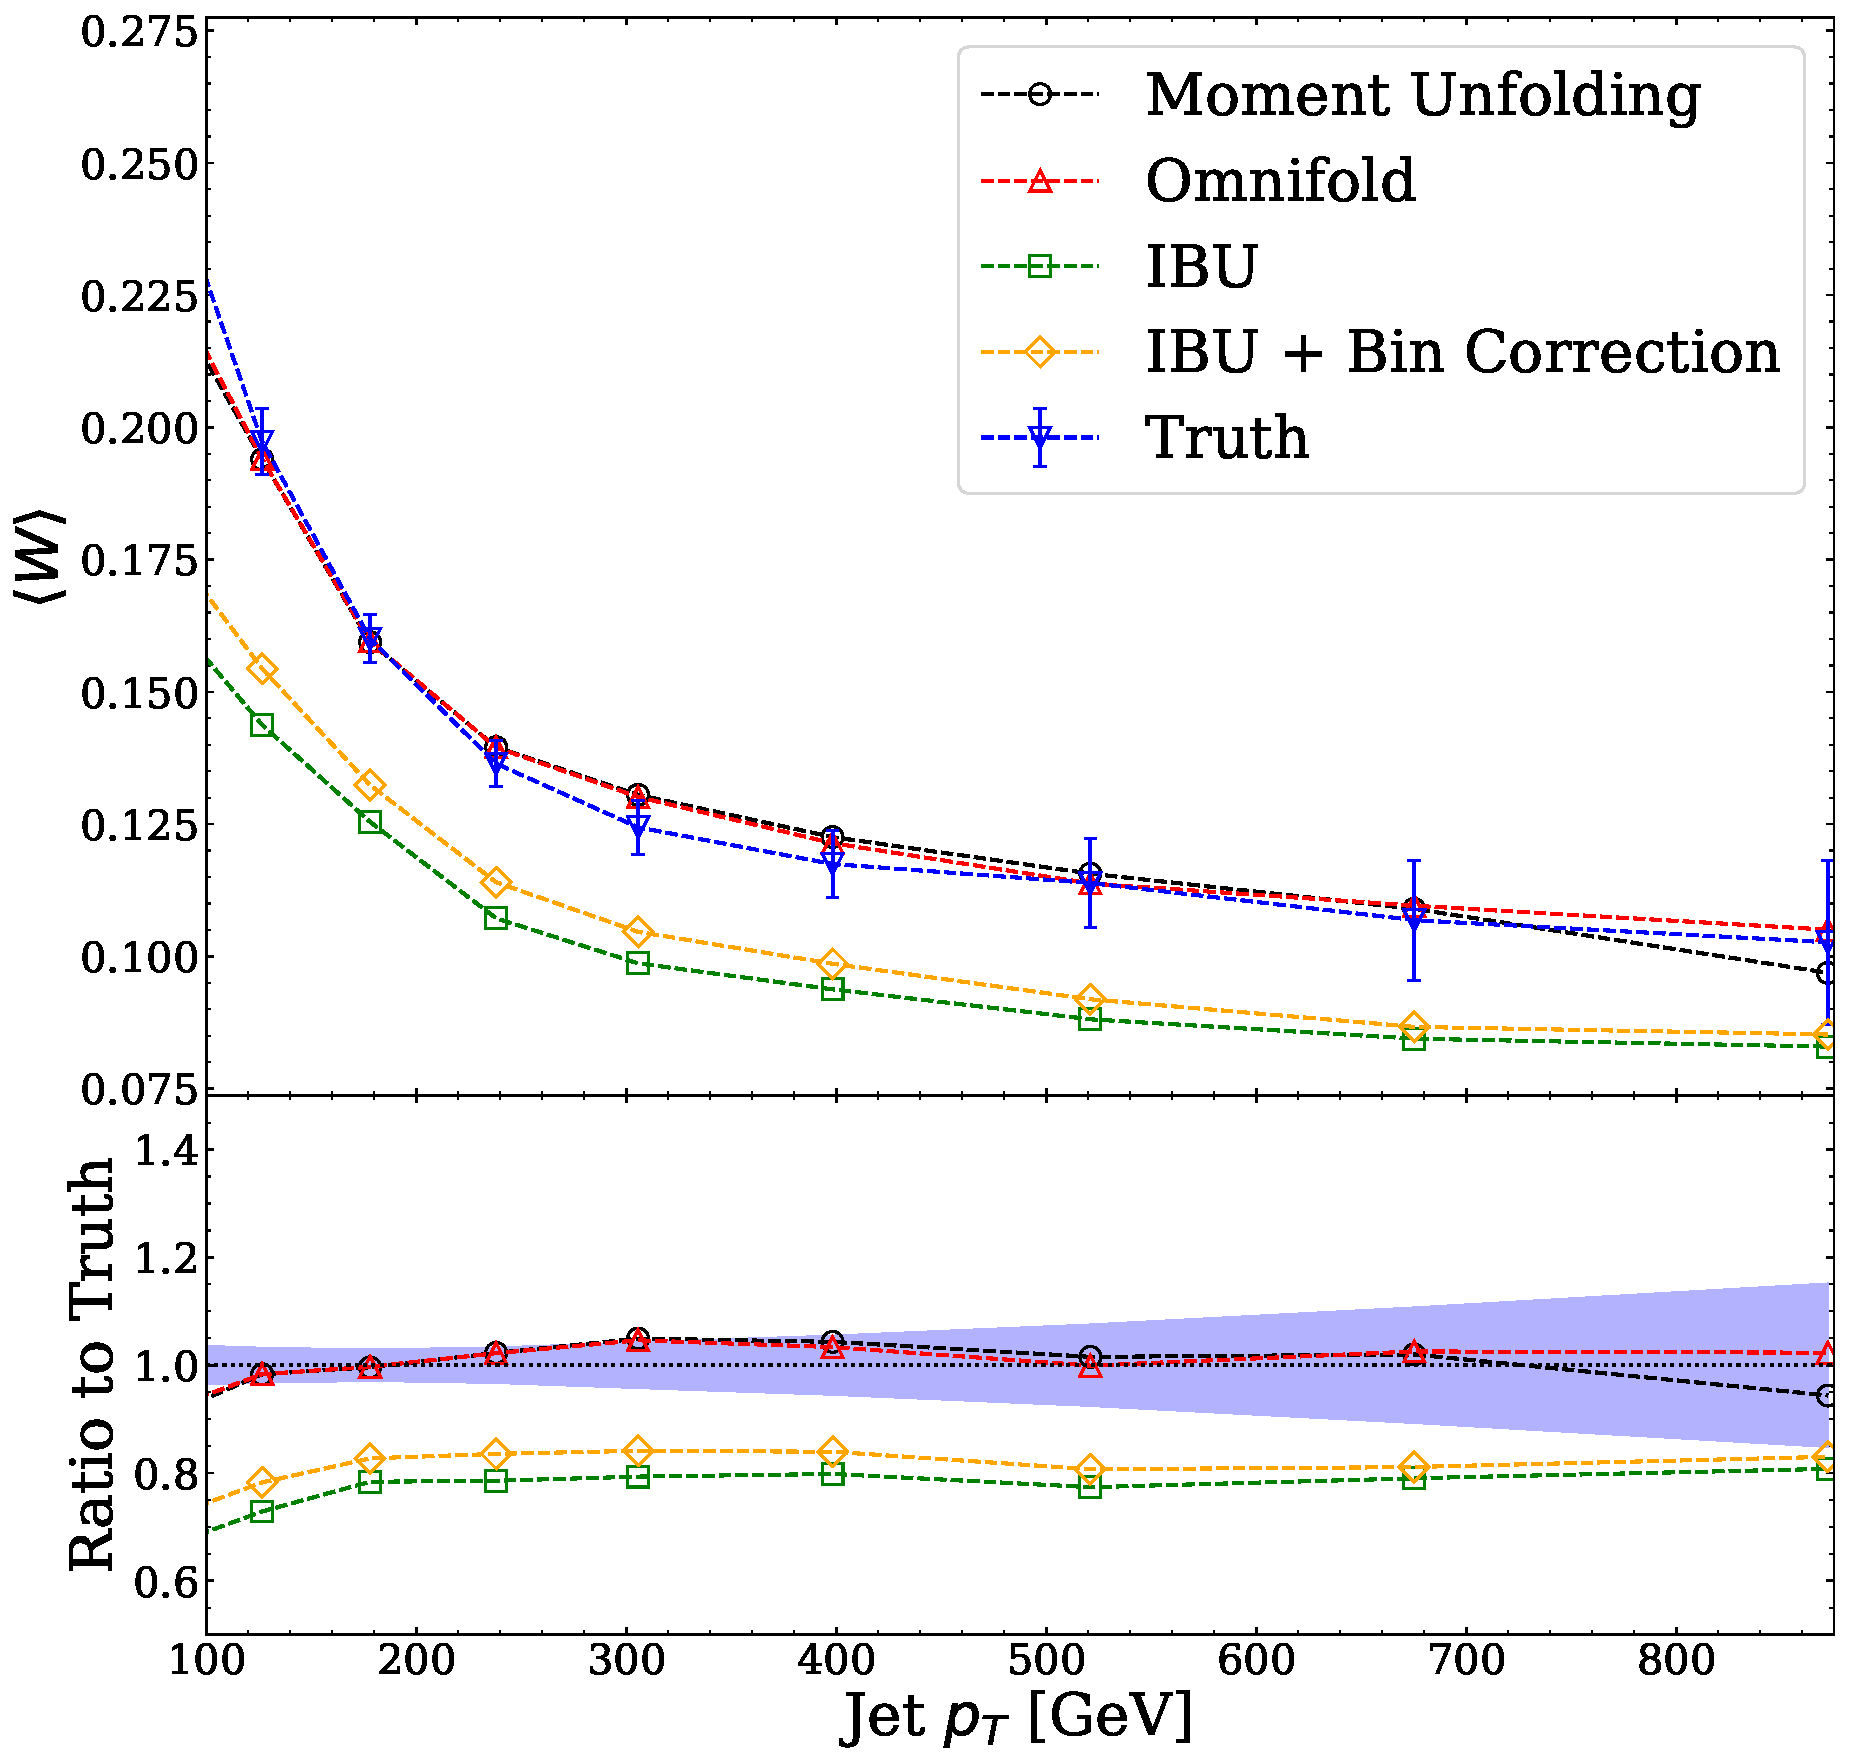
\includegraphics[height=0.45\textwidth]{figures/chapter-05/moment1_w_v_pT.pdf}}
    \subfloat[]{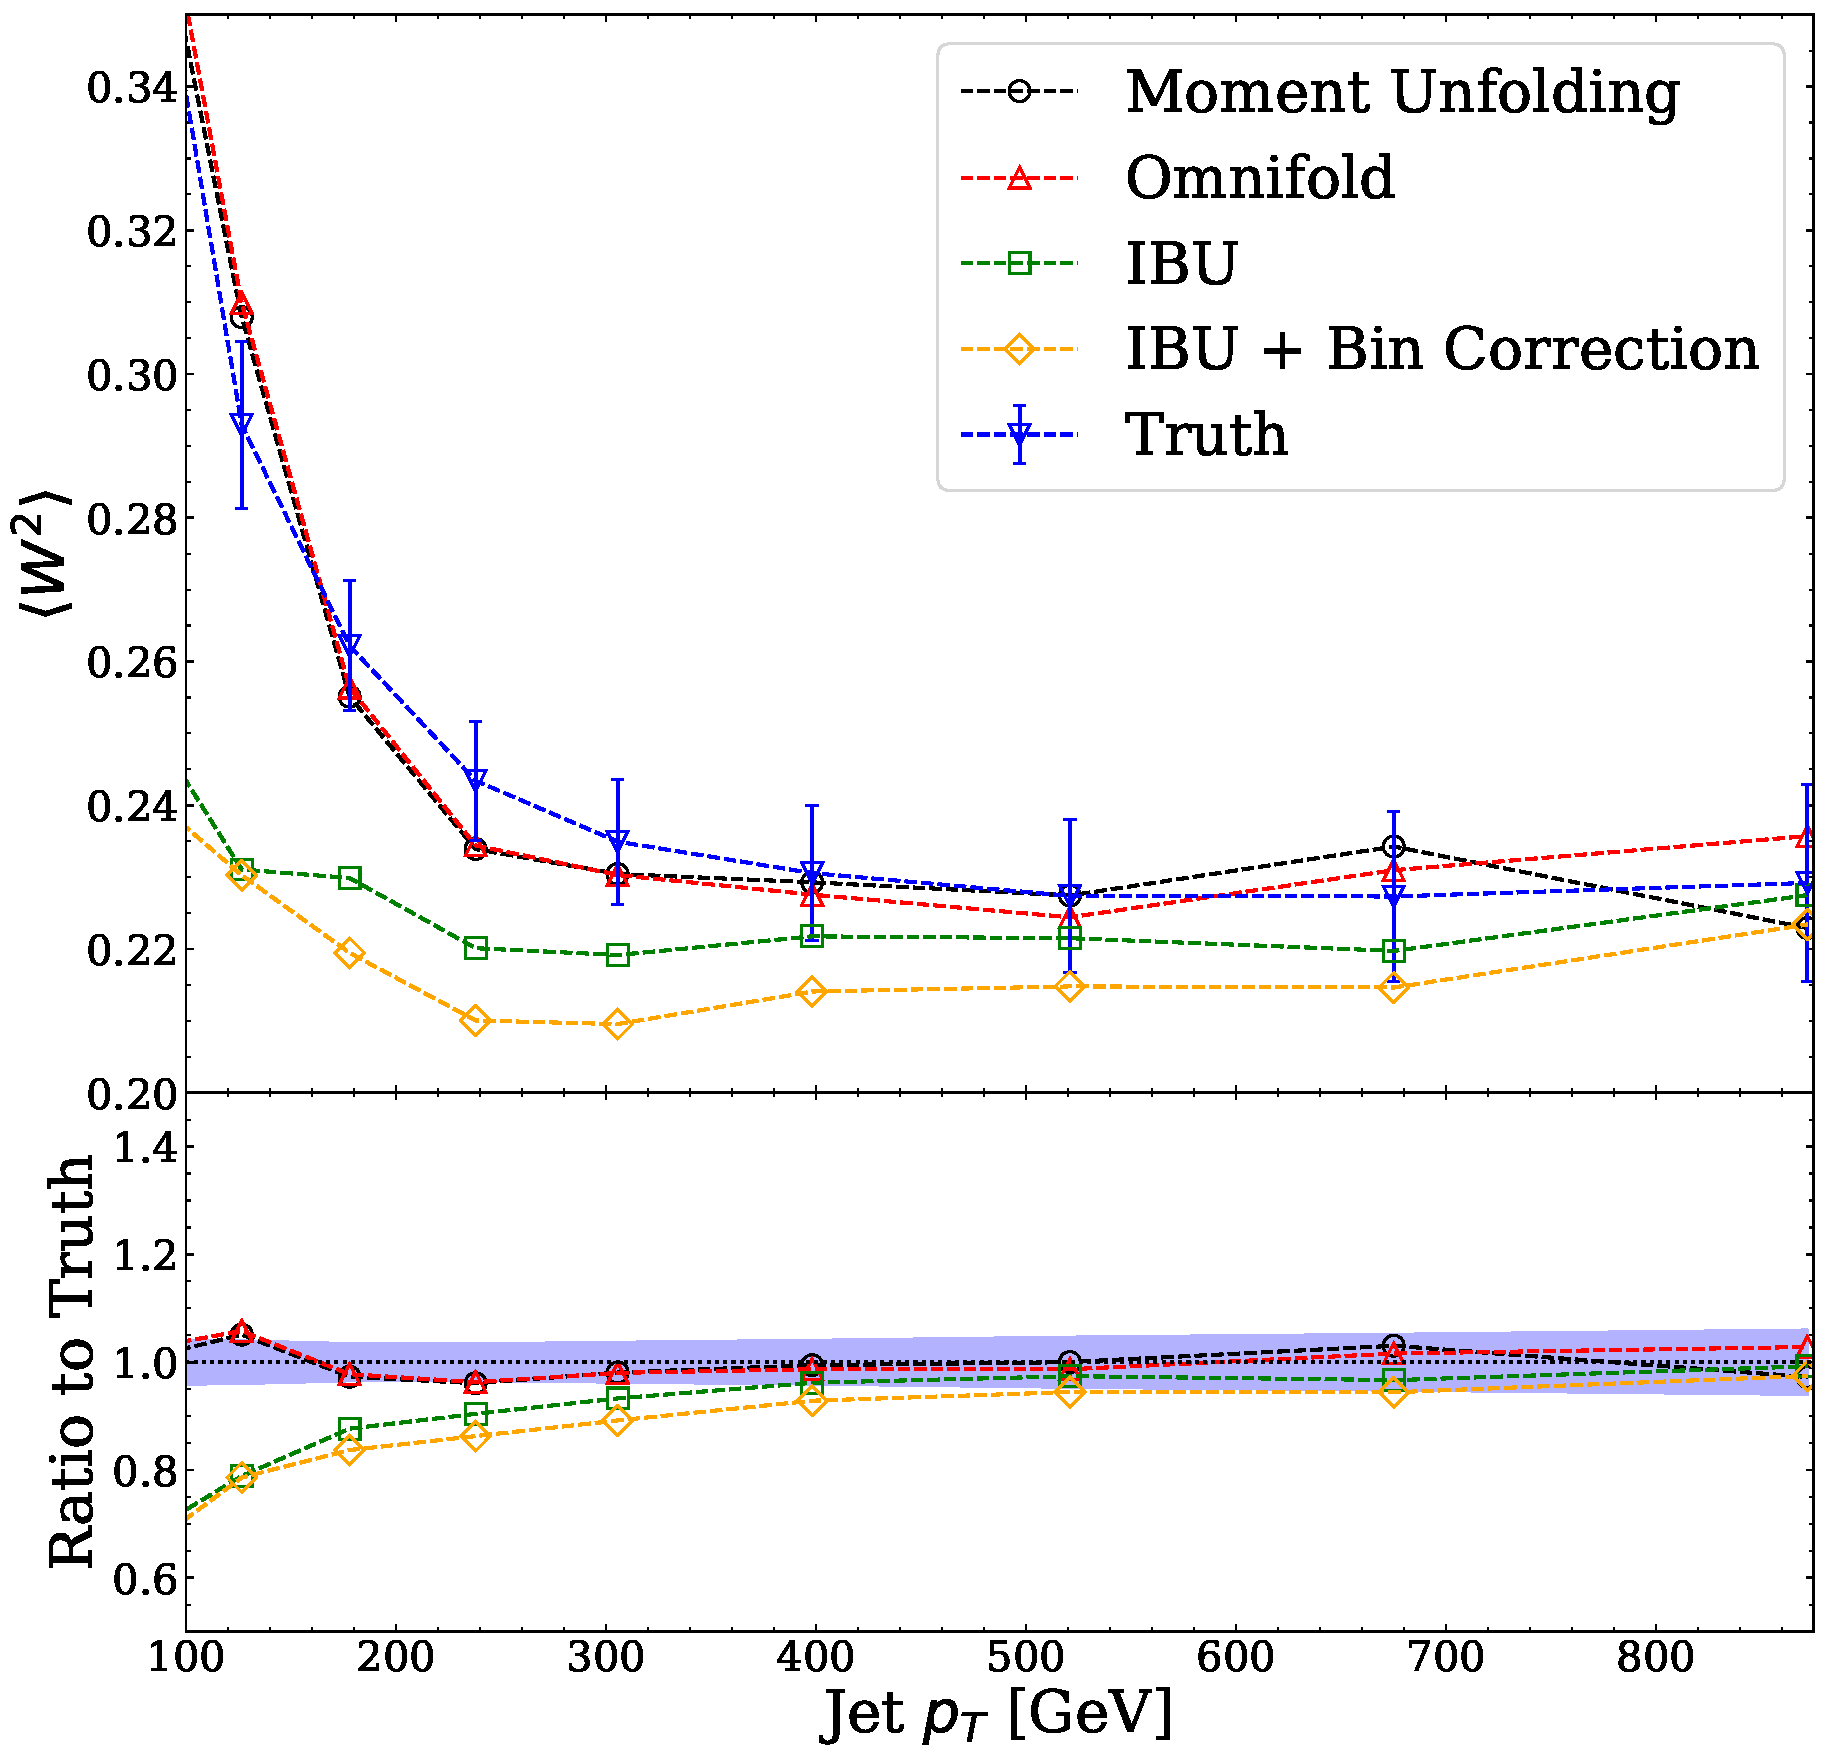
\includegraphics[height=0.45\textwidth]{figures/chapter-05/moment2_w_v_pT.pdf}}\\

    \subfloat[]{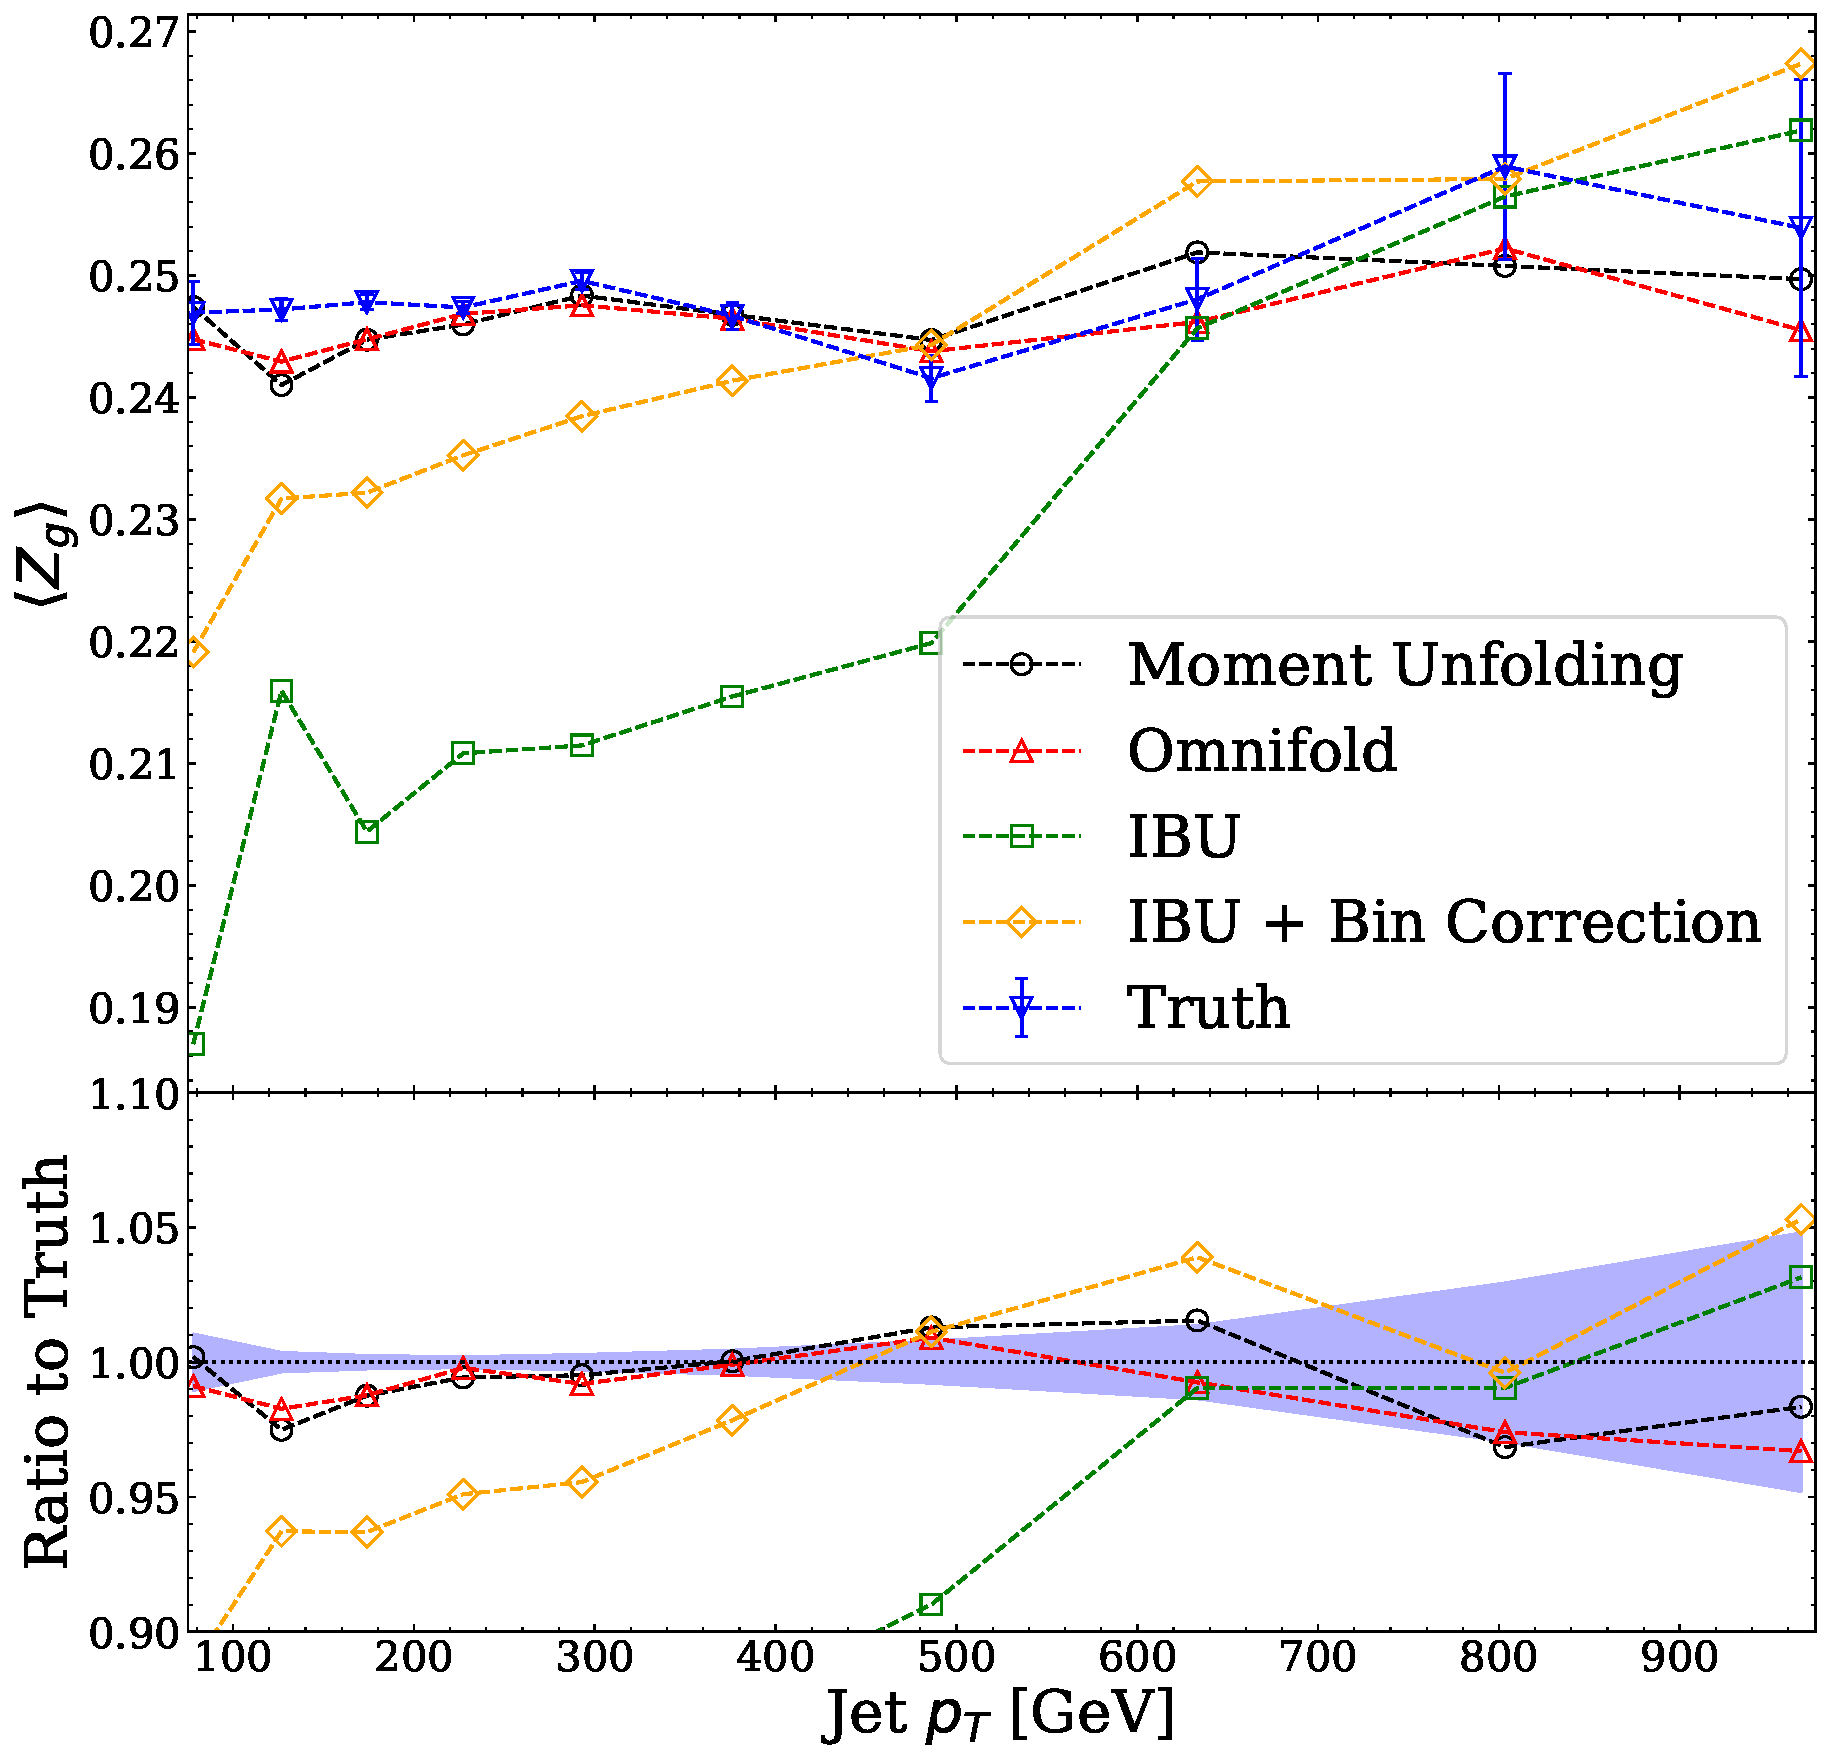
\includegraphics[height=0.45\textwidth]{figures/chapter-05/moment1_zg_v_pT.pdf}}
    \subfloat[]{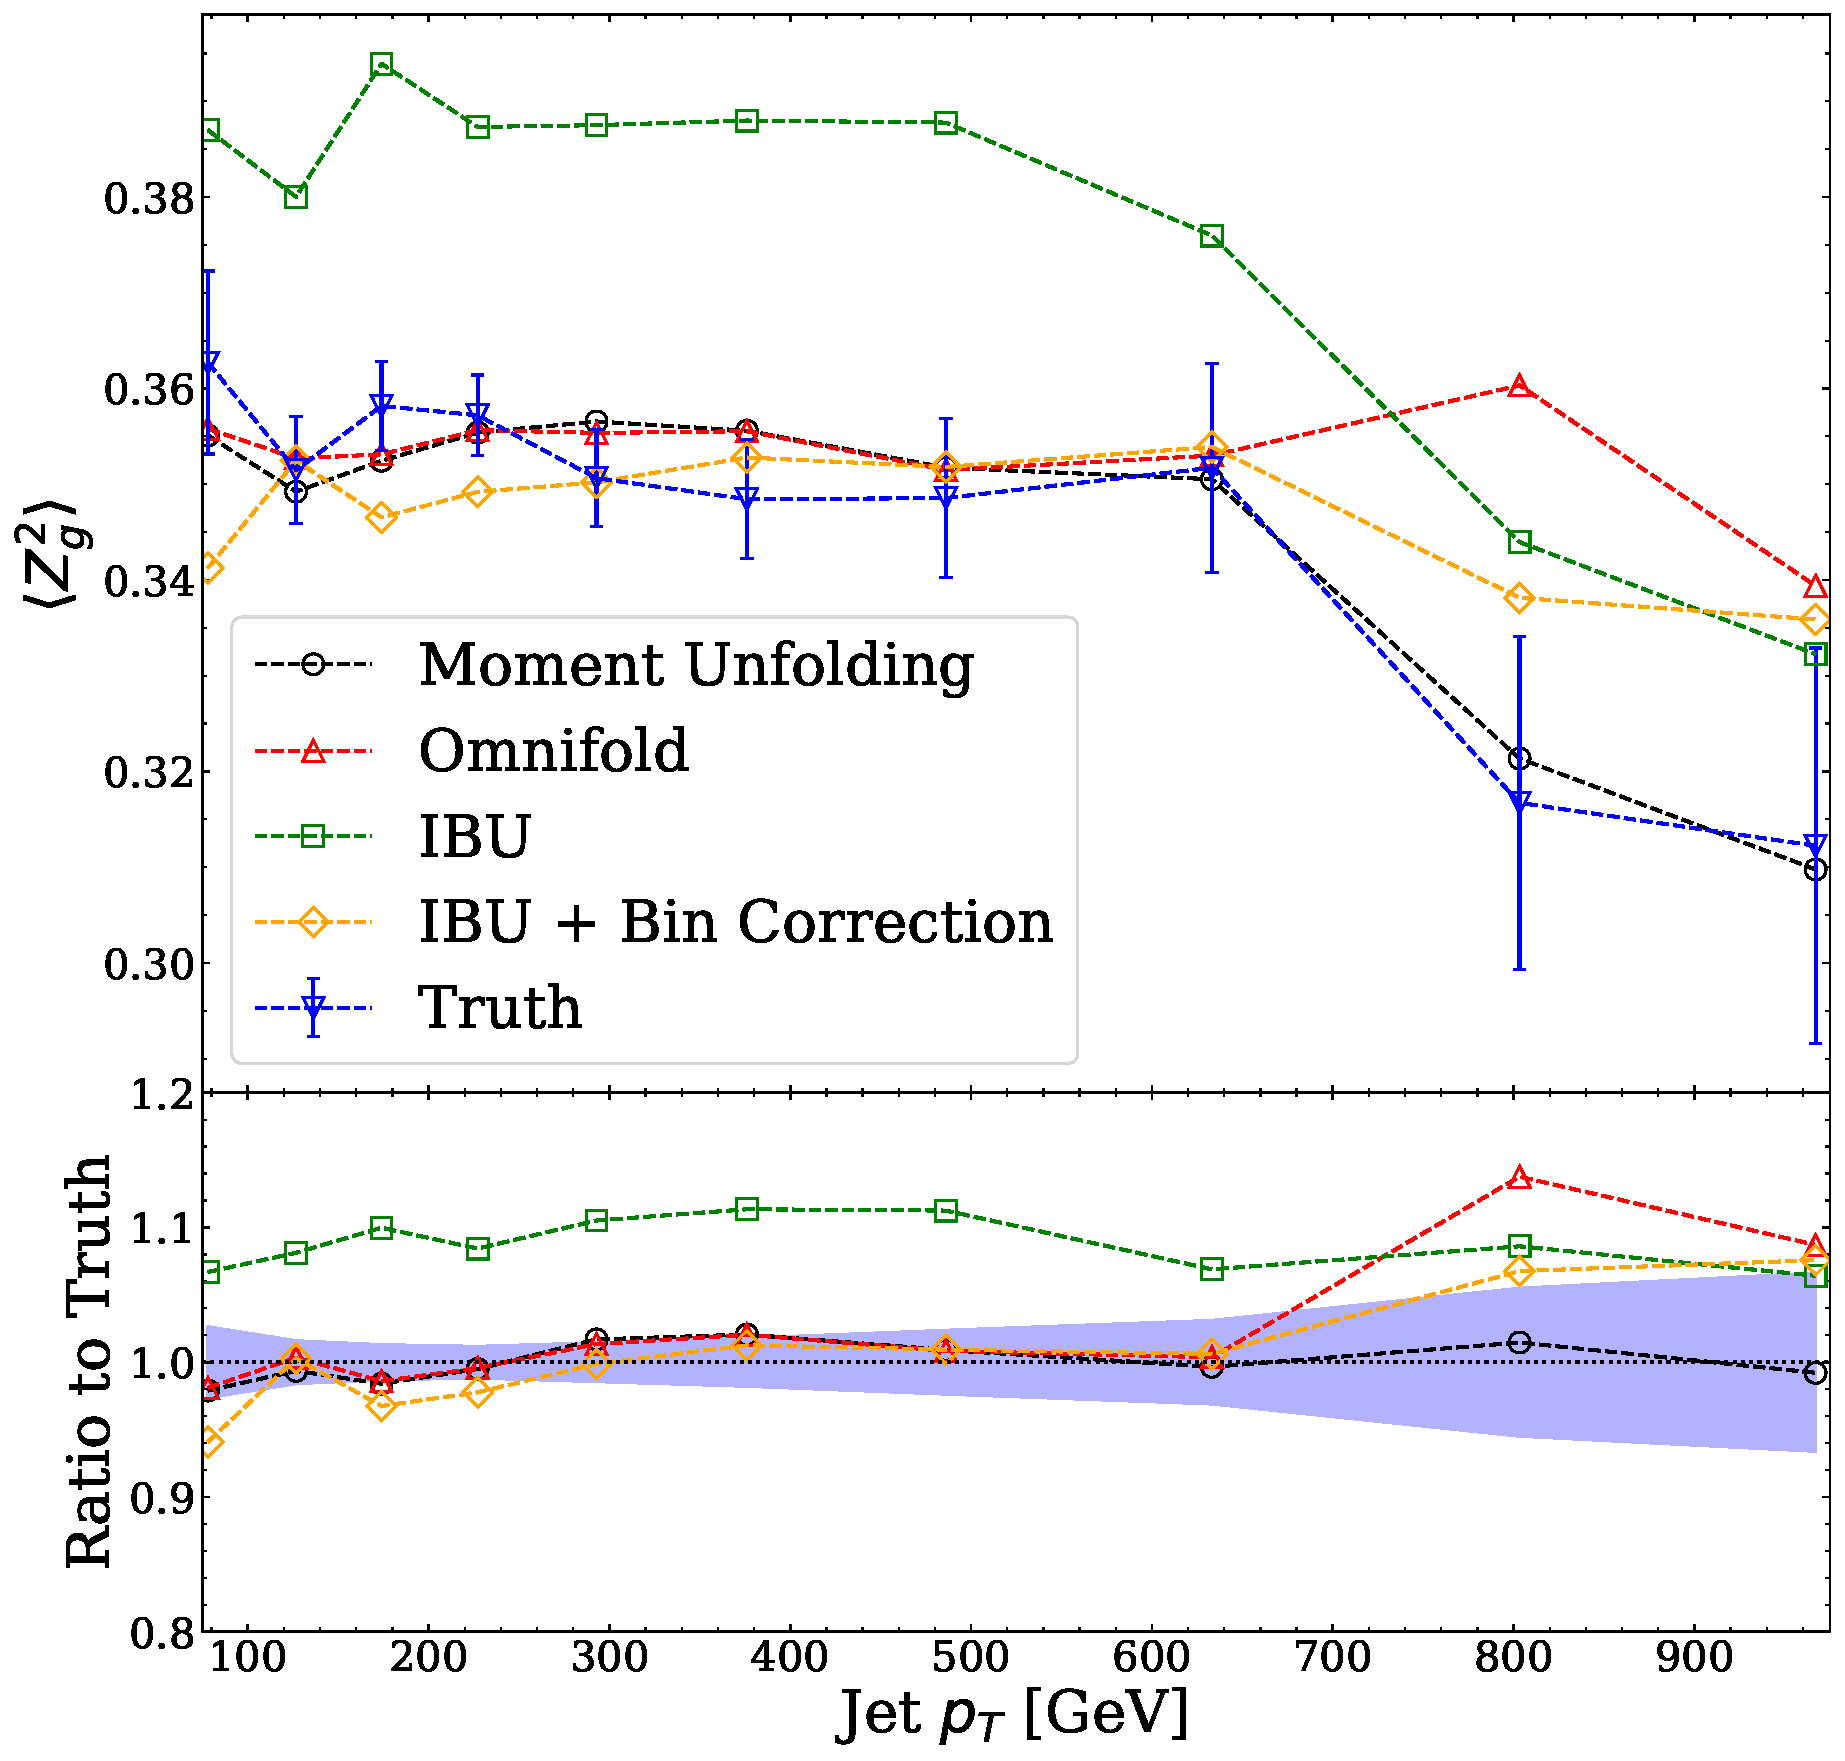
\includegraphics[height=0.45\textwidth]{figures/chapter-05/moment2_zg_v_pT.pdf}}
    
    \caption[]{(Continued.) Mean (left column) and variance (right column) for (e,f) jet width and (g,h) groomed momentum fraction. Methods compared include \textsc{Moment Unfolding}, OmniFold, Iterative Bayesian Unfolding (IBU), and IBU with bin-by-bin corrections. The lower panel in each plot shows the ratio to truth, highlighting that \textsc{Moment Unfolding} achieves precision comparable to OmniFold while significantly outperforming IBU, particularly at high $p_T$ where binning effects become more pronounced.}
\end{figure}

    For a comprehensive comparison, we also include a variation on IBU that applies bin by bin corrections to account for binning effects in the moment calculation.
    %
    \cref{fig:method-comparison} shows the moments of each observable as a function of jet $p_T$ for all methods, comparing them to the true values.
    %
    The lower panels show the ratio to truth, highlighting differences between methods.

    This comparison highlights some of \textsc{Moment Unfolding}'s most important properties.
    %
    The \textsc{Moment Unfolding} algorithm achieves comparable or better precision than \textsc{\textsc{OmniFold}} for most observables, despite, or perhaps due to, its more targeted approach.
    %
    This demonstrates the advantage of directly targeting the moments without having to unfold the entire distribution.
    %
    Both unbinned methods (\textsc{Moment Unfolding} and \textsc{\textsc{OmniFold}}) significantly outperform the binned approaches (IBU and IBU+Correction) in precision, highlighting the benefits of avoiding binning artifacts.
    %
    The bin--by--bin correction improves the performance of IBU but still does not match the precision of the unbinned methods, indicating that the fundamental limitations of binning cannot be fully mitigated by \textit{post hoc} corrections.
    
    However, \textsc{Moment Unfolding} requires significantly less computational resources than \textsc{\textsc{OmniFold}} due to its non-iterative nature.
    %
    On average, \textsc{Moment Unfolding} can be run in about 1\% of the time required for {\textsc{OmniFold}}, while achieving comparable or better precision.
    %
    This comparison highlights the practical advantages of \textsc{Moment Unfolding} in scenarios where computational resources are limited or where multiple unfolding tasks need to be performed, such as in systematic uncertainty studies.
    %
    That said, IBU is about \(\num{d4}\) times faster than \textsc{Moment Unfolding}, so in analyses where computation is at a high premium, and the binning artifacts introduced by IBU are acceptable, IBU continues to offer a low--tech, light unfolding procedure.

    These results establish \textsc{Moment Unfolding} as a powerful tool for precision measurements of statistical moments in high energy physics, offering advantages in both statistical precision and computational efficiency compared to existing methods.

\section{Conclusion.}
    \textsc{Moment Unfolding} represents a significant advancement in the statistical toolkit for particle physics measurements, providing a novel approach to directly extract moments of distributions without the intermediate step of reconstructing the full spectrum.
    %
    This methodology addresses several challenges in traditional unfolding techniques while offering unique advantages for theoretical comparison and interpretation.
    %
    An intrinsically unbinned method, \textsc{Moment Unfolding} eliminates binning artifacts and dimensionality limitations that affect traditional methods.
    %
    By using a physically motivated reweighting function based on the Boltzmann distribution, it provides a principled approach to the unfolding problem, with clear connections to the maximum entropy principle from statistical mechanics.

    The adversarial training framework effectively addresses the two level nature of the unfolding problem, allowing corrections to particle level simulation to be optimised based on detector level comparisons between measured and simulated distributions.
    %
    By extending this basic architecture to unfold moments conditional on momentum, \textsc{Moment Unfolding} can be used for detailed studies of how moments scale with energy, providing powerful constraints on theoretical models.
    
    As a non-iterative method that is designed specifically to unfold moments rather than full spectra, \textsc{Moment Unfolding} offers significant computational advantages over iterative approaches, particularly for systematic uncertainty studies that require multiple unfolding runs.
    %
    The application to jet substructure measurements in Sec.~\ref{subsec:jet-moments} demonstrates the practical utility of \textsc{Moment Unfolding} for real physics analyses.
    %
    The method successfully recovers both inclusive and differential moments of diverse jet observables, providing enhanced precision compared to traditional binned approaches and comparable or better accuracy than full-distribution unbinned methods.
    %
    These capabilities make \textsc{Moment Unfolding} particularly valuable for precision tests of QCD, where theoretical predictions are often most precise at the level of moments rather than full distributions.
    
    Although \textsc{Moment Unfolding} excels at extracting moments, it does not guarantee optimal reconstruction of the full distribution, particularly when higher moments are significant.
    %
    The choice of how many moments to unfold represents a regularization parameter that must be carefully selected based on the physics application and available statistics.
    %
    The basic formulation discussed above is designed for moments of a single observable, though extensions to joint moments are possible.
    \subsection{Towards unfolding distributions.}
        While \textsc{\textsc{Moment Unfolding}} offers significant advantages for moment specific measurements, many analyses do require the full unfolded distribution rather than just its moments.
        %
        This raises the question: can the Boltzmann inspired approach be extended to unfold entire distributions?
        %
        In a sense, this should be relatively straightforward.
        %
        If the degree of the polynomial in the exponent of the Boltzmann factor governs the number of moments unfolded, by simply replacing the polynomial with a Taylor series,
        \[
            g(z) = \frac{1}{P}\exp\left[-\sum_{a=1}^{\infty}\beta_a z^a\right],
        \]
        we could, in principle, constrain all moments simultaneously, thereby unfolding the entire distribution.
        %
        Even if this were not feasible, by Taylor's theorem~\cite{taylor_methodus_1715} in conjunction with the Hausdorff moment uniqueness theorem~\cite{Hausdorff1921} and the Stone-Weierstrass approximation theorem~\cite{weierstras_uber_1885, pani_generalized_2024}, for any arbitrary precision \(\epsilon\), there exists a sufficiently high number of moments \(n\) such that the Hausdorf reconstruction from \(n\) or more moments approximates the probability density with precision better than \(\epsilon.\)
        %
        So even if it were for some reason it were not possible to unfold infinitely many moments, as long as it were possible to unfold arbitrarily large finite numbers of moments, that would provide us with a solution to this problem as well.
        
        However, since the degree of the polynomial is precisely the regularising parameter for the inverse problem in the \textsc{Moment Unfolding} approach, by increasing it (to some large number or infinity) this approach lifts the regularisation central to the algorithm.
        %
        The resulting ill posed inverse problem requires significant regularisation.

        These challenges motivate the development of the Reweighting Adversarial Network (RAN) method, which will be introduced in \cref{chap:ran}.
        %
        RAN builds upon the foundations laid by \textsc{Moment Unfolding}, extending the approach to full distribution unfolding while maintaining its unbinned, non-iterative, adversarial nature.
        %
        By incorporating more flexible neural network parametrisations and Wasserstein metrics for distribution comparison, RAN addresses the limitations of \textsc{Moment Unfolding} while preserving its core strengths.
        %
        This evolution from moment specific to full distribution unfolding represents a natural progression in developing a comprehensive framework for unbinned cross section measurements in particle physics.